\documentclass{auxiliares/umemoria} 
%%%%%%%%%%%%%%%%%%%%%%%%%%%%%%%% INFORMACIÓN DE PORTADA %%%%%%%%%%%%%%%%%%%%%%%%%%%%%%%%%%%%%%%%%%%%%%%%
\depto{Departamento de Ingeniería Mecánica} % Nombre del Departamento
\author{Diego Andrés Concha Araya} % Nombre del autor
\title{Simulación de parámetros operativos de{\vspace{1.5ex}\break}ventilador minero para aplicaciones en{\vspace{1.5ex}\break}mantenimiento predictivo basado en machine learning}  % Ajustar título a gusto con {\vspace{1.5ex}\break}
%\bajadatitulo{Entrega 16/03/2025} % Bajada de titulo (eliminar al enviar a biblioteca)
\titulopdf{Tesis Diego Concha}  % Nombre Asignado al PDF
\tesis{Ingeniero Civil en Mecánica} % Grado al que opta
\guia{Michael Miranda Sandoval}   % Profesor guía 
\anho{2024}     % Año en que se da el examen de título/grado (defensa) o ultima matricula de pregrado
%%%%%%%%%%%%%%%%%%%%%%%%%%%%%%%%%%%%%%%%%%%%%%%%%%%%%%%%%%%%%%%%%%%%%%%%%%%%%%%%%%%%%%%%%%%%%%%%%%%%%%%%%

% Lugar donde se encuentra la bibliografía
\addbibresource{library.bib}
% Hints: formulas que se repiten como notaciones de vectores que son muy extensas de escribir en cada apartado
\newcommand{\prob}{\mathbb{P}}
\newcommand{\E}{\mathbb{E}}
\newcommand{\V}{\mathbb{V}}
\newcommand{\distribuyeiid}{\overset{{iid}}{\sim}}

\newcommand{\error}{\varepsilon}
\newcommand{\SE}{{\sigma^2}}
\newcommand{\B}{\beta}
\newcommand{\A}{\alpha}
\newcommand{\vcero}{\vec{0}} 

    %PÁGINAS PRELIMINARES
%%%%%%%%%%%%%%%%%%%%%%%%%%%%%%%%%%
%(1) PORTADA 			
%(2) DERECHOS DE AUTOR 		
%(3) RESUMEN Y ABSTRACT 	
%(4) DEDICATORIA(OPTATIVA)
%(5) AGRADECIMIENTOS(OPTATIVA)	
%(6) TABLA DE CONTENIDOS
%(7) ÍNDICE DE TABLAS	
%(8) ÍNDICE DE ILUSTRACIONES
%%%%%%%%%%%%%%%%%%%%%%%%%%%%%%%%%%


% %%deja la pagina del apéndice sin numero
\let\plainappendixpage\appendixpage
 \makeatletter
 \renewcommand{\appendixpage}{%
  \begingroup
  \let\ps@plain\ps@empty
  \plainappendixpage
  \endgroup}
\makeatother

%Comandos para apéndice
\renewcommand{\appendixname}{Ap\'endice}
\renewcommand{\appendixtocname}{Ap\'endices y anexos}
\renewcommand{\appendixpagename}{AP\'ENDICES Y ANEXOS}


%%%%%%%%%%%%%%%%%%%%%%%%%%%%%%%%%%%%% INICIO PAGINAS PRELIMINARES %%%%%%%%%%%%%%%%%%%%%%%%%%%%%%%%%%%%%%%
%%%%%%%%%%%%%%%%%%%%%%%%%%%%%%%%%%%%%%%%%%%%%%%%%%%%%%%%%%%%%%%%%%%%%%%%%%%%%%%%%%%%%%%%%%%%%%%%%%%%%%%%%
\begin{document}
\onehalfspacing
\frontmatter
\maketitle
%%%%%%%%%%%%%%%%%%%%%%%%%%%%%%%%%%%%%%%%%%%%%%%%%%%%%%%%%%%%%%%%%%%%%%%%%%%%%%%%%%%%%%%%%%%%%%%%%%%%%%%%%
% Derechos de autor / omitir cuando se envía a biblioteca
%\begin{derechoautor}
%\copyright \,Diego Concha Araya, 2025.\\
%\textbf{Todos los derechos reservados. Chile.}
%\end{derechoautor}
%%%%%%%%%%%%%%%%%%%%%%%%%%%%%%%%%%%%%%%%%%%%%%%%%%%%%%%%%%%%%%%%%%%%%%%%%%%%%%%%%%%%%%%%%%%%%%%%%%%%%%%%%
% Resumen breve
\begin{resumen}

  El objetivo principal de este trabajo es desarrollar un modelo a escala de un túnel de viento análogo a un sistema de ventilación minera, incorporando un controlador programado en Arduino para regular la velocidad del ventilador y realizar la adquisición de datos. Con dichos datos, se construye un modelo de Dinámica de Fluidos Computacional (CFD) con el fin de estudiar el flujo de aire y predecir comportamientos operativos bajo distintas condiciones.

  La validación del modelo se efectúa comparando las velocidades de viento medidas con sensores calibrados frente a los valores teóricos de la simulación a diferentes velocidades de giro (RPM) del ventilador. Este enfoque tiene como finalidad proveer una plataforma experimental y computacional que contribuya a optimizar el rendimiento de sistemas de ventilación, así como a plantear futuros esquemas de mantenimiento predictivo y automatización basados en la correlación entre datos reales y simulaciones.
\end{resumen}

\vfill
\noindent\textbf{Palabras claves: } Túnel de viento, Ventilación minera, Simulación CFD, Arduino, Mantenimiento predictivo, Validación experimental.  % cada palabra comienza con mayúscula separadas por coma.
%%%%%%%%%%%%%%%%%%%%%%%%%%%%%%%%%%%%%%%%%%%%%%%%%%%%%%%%%%%%%%%%%%%%%%%%%%%%%%%%%%%%%%%%%%%%%%%%%%%%%%%%%
% Abstract
\begin{abstract}
  The main objective of this study is to develop a scaled wind tunnel model analogous to a mining ventilation system, integrating an Arduino-based controller for fan speed regulation and data acquisition. These data are then used to build a Computational Fluid Dynamics (CFD) model aimed at analyzing airflow and predicting operational behavior under various conditions.

  Model validation is carried out by comparing wind velocities measured by calibrated sensors against theoretical simulation values at different fan speeds (RPM). This approach provides both an experimental and computational platform to optimize ventilation system performance and to propose future predictive maintenance and automation strategies based on the correlation between real data and simulations.\\

\end{abstract}
\vfill
\noindent\textbf{Keywords: } Wind tunnel, Mining ventilation, CFD simulation, Arduino, Predictive maintenance, Experimental validation.

%%%%%%%%%%%%%%%%%%%%%%%%%%%%%%%%%%%%%%%%%%%%%%%%%%%%%%%%%%%%%%%%%%%%%%%%%%%%%%%%%%%%%%%%%%%%%%%%%%%%%%%%%
% Dedicatoria corta o frase inspiradora, poema, etc.

\begin{dedicatoria}
``A mi pequeña familia,
por ser raíz, abrigo y fuerza en cada paso.

A quienes, con su ejemplo y palabra,
me mostraron el verdadero significado del esfuerzo y la dedicación.

Y en especial, a mi tío Edward Araya,
que con su memoria viva me enseñó
que el ingenio no solo está en las ideas,
sino en el corazón que las impulsa.''
\end{dedicatoria}

%%%%%%%%%%%%%%%%%%%%%%%%%%%%%%%%%%%%%%%%%%%%%%%%%%%%%%%%%%%%%%%%%%%%%%%%%%%%%%%%%%%%%%%%%%%%%%%%%%%%%%%%%
% Agradecimientos

\begin{thanks}
Al llegar al cierre de esta etapa tan significativa en mi vida académica y personal, quiero expresar mi más sincero agradecimiento a todas aquellas personas que hicieron posible este logro.

En primer lugar, a mi profesor guía y mentor Michael Miranda, por su invaluable apoyo, guía constante y dedicación durante todo el desarrollo de esta tesis. Su compromiso, exigencia y confianza fueron claves para que este trabajo alcanzara la profundidad y calidad esperadas.

A todo el equipo de desarrollo del proyecto FAS, en especial a su director Sebastián Pérez, por brindarme la oportunidad de participar activamente en un entorno profesional enriquecedor, donde pude aplicar y expandir mis conocimientos.

A mi familia más cercana, quienes han sido un pilar fundamental a lo largo de este proceso: a mi madre María Eugenia Araya, por su amor incondicional y constante aliento; a mi padrino Carlos Chávez, por su apoyo y consejos sabios; y a mi tía y madrina Nena Cerezo, por estar siempre presente con palabras de ánimo y cariño.

También quiero agradecer profundamente a todos los profesores de la Facultad de Ingeniería Mecánica que contribuyeron a mi formación integral. Cada uno, con su vocación y compromiso, dejó una huella en mi camino profesional y personal.

Por último, a mis compañeras y compañeros de la casa de estudios que me acompañaron y apoyaron a lo largo de estos años. Su compañía, colaboración y amistad fueron esenciales para sobrellevar los desafíos y disfrutar los logros del camino recorrido.

A todos y todas, gracias de corazón.
\end{thanks}

%%%%%%%%%%%%%%%%%%%%%%%%%%%%%%%%%%%%%%%%%%%%%%%%%%%%%%%%%%%%%%%%%%%%%%%%%%%%%%%%%%%%%%%%%%%%%%%%%%%%%%%%%
\cleardoublepage
% INDICE

\phantomsection
\tableofcontents % índice general
\addcontentsline{toc}{chapter}{Tabla de Contenido}
\listoftables % índice de tablas
\addcontentsline{toc}{chapter}{Índice de Tablas}
\listoffigures % índice de figuras
\addcontentsline{toc}{chapter}{Índice de Figuras}
\pagebreak

%%%%%%%%%%%%%%%%%%%%%%%%%%%%%%%%%%%%%%%%%%%%%%%%%%%%%%%%%%%%%%%%%%%%%%%%%%%%%%%%%%%%%%%%%%%%%%%%%%%%%%%%%
%%%%%%%%%%%%%%%%%%%%%%%%%%%%%%%%%%%%% FIN PAGINAS PRELIMINARES %%%%%%%%%%%%%%%%%%%%%%%%%%%%%%%%%%%%%%%%%%

\mainmatter
\chapter{Introducción}

El proceso de ventilación minera juega un papel fundamental en la seguridad y eficiencia de la explotación subterránea. En entornos mineros, el control del flujo de aire es esencial para mantener condiciones de trabajo óptimas, garantizar la extracción de gases nocivos y reducir la temperatura generada por la maquinaria y el personal. Los ventiladores representan el corazón de estos sistemas, y su desempeño influye de forma directa en la calidad del ambiente subterráneo y en los costos de operación y mantenimiento \cite{Zhou2020, Sanchis2022}.

En el presente trabajo, se plantea el desarrollo de un túnel de viento a escala que simula de manera análoga el funcionamiento de un sistema de ventilación minera. Este prototipo integra un ventilador regulado por un controlador basado en Arduino, así como un conjunto de sensores que permiten medir parámetros operativos como corriente, voltaje, vibración, temperatura y flujo de aire. A partir de dichos datos, se construye un modelo de Dinámica de Fluidos Computacional (CFD) con el fin de validar la precisión de las simulaciones frente a los registros experimentales \cite{ANSYS2021}. Este enfoque posibilita el estudio detallado de la distribución del flujo de aire dentro del sistema y la identificación de condiciones operativas óptimas, así como el análisis de potenciales fallas o anomalías.

El objetivo central de la tesis es establecer una aproximación para el mantenimiento predictivo de sistemas de ventilación minera a partir de la correlación entre los datos obtenidos en el prototipo y los resultados de simulación. Con un control y una adquisición de datos en tiempo real, se busca detectar de manera temprana posibles condiciones de mal funcionamiento o estados de degradación del equipo, sentando las bases para futuros estudios que involucren la implementación de modelos de machine learning o algoritmos de diagnóstico avanzado.

\section{Motivación y Justificación}
La industria minera, y en particular la que opera en espacios subterráneos, enfrenta retos constantes relacionados con la calidad del aire y la eficiencia energética. La necesidad de reducir costos operativos, junto con el imperativo de mantener la seguridad de los trabajadores, ha motivado el desarrollo de sistemas de ventilación más fiables y eficientes \cite{Zhou2020}. No obstante, la validación de estos sistemas mediante pruebas a gran escala puede ser costosa y compleja, especialmente en entornos mineros activos.

En este contexto, la implementación de un túnel de viento a escala representa una alternativa viable para la experimentación. El uso complementario de simulaciones CFD posibilita la comprensión de la dinámica del flujo de aire, así como el análisis de escenarios de operación y la detección temprana de condiciones potencialmente peligrosas. Al comparar los datos reales del prototipo con los resultados de simulación, se aporta un método objetivo para el diseño y la evaluación de esquemas de mantenimiento predictivo en ventiladores mineros \cite{Sanchis2022}.

\section{Planteamiento del Problema}
En la práctica, gran parte de los planes de mantenimiento de ventiladores mineros se ejecutan de manera preventiva, basándose en ciclos de reemplazo o revisión establecidos. Dichos planes no siempre reflejan el estado real de la maquinaria, dando lugar a un sobredimensionamiento de las intervenciones o, en su defecto, a fallos imprevistos que incrementan los costos de operación y el riesgo de accidentes. Existe, por tanto, la necesidad de desarrollar un método que permita correlacionar mediciones en tiempo real (vibraciones, temperaturas críticas, flujo de aire y consumo eléctrico) con modelos de simulación, a fin de anticipar potenciales fallas y reducir las paradas no planificadas.

Para abordar esta problemática, se propone la construcción de un túnel de viento a escala que, a través de un sistema de adquisición de datos y de un modelo CFD, permita establecer una línea base de comportamiento normal. Sobre dicha línea base, sería posible identificar derivaciones anómalas e implementar estrategias de mantenimiento predictivo con mayor efectividad.

\section{Objetivos}
\subsection{Objetivo General}
Diseñar e implementar un modelo a escala de un túnel de viento con analogía a sistemas de ventilación minera, con instrumentación y control basados en Arduino, a fin de evaluar y correlacionar datos de operación con un modelo de Dinámica de Fluidos Computacional (CFD) para el desarrollo de estrategias de mantenimiento predictivo.

\subsection{Objetivos Específicos}
\begin{itemize}
    \item \textbf{Diseñar y construir el prototipo a escala:} Elaborar la estructura del túnel de viento y el sistema de ventilación, considerando aspectos geométricos y operativos que se asemejen a los conductos y ventiladores de la industria minera.
    \item \textbf{Integrar la instrumentación y el control:} Seleccionar e instalar sensores de corriente, voltaje, temperatura, vibración y flujo de aire, así como programar el microcontrolador Arduino para gestionar y registrar en tiempo real los datos del sistema.
    \item \textbf{Desarrollar el modelo CFD:} Configurar y ejecutar la simulación en software especializado, como ANSYS, para modelar la dinámica del flujo de aire y las condiciones térmicas y estructurales del prototipo a distintas RPM del ventilador.
    \item \textbf{Comparar datos experimentales y simulación:} Validar el modelo CFD mediante la comparación de los valores obtenidos en pruebas experimentales con las predicciones numéricas en diversas condiciones operativas.
    \item \textbf{Proponer lineamientos de mantenimiento predictivo:} Basarse en la correlación entre las mediciones del prototipo y la simulación para formular recomendaciones que puedan extrapolarse a sistemas de ventilación a escala real.
\end{itemize}

\newpage
\section{Alcance y Limitaciones}
El presente estudio se circunscribe al diseño, construcción y validación de un túnel de viento a escala que reproduce de manera simplificada un sistema de ventilación minera. El análisis de resultados se enfoca en la medición de parámetros como corriente, voltaje, vibración, flujo de aire y temperatura, sin abarcar modificaciones sustanciales en la geometría de las palas del ventilador o la implementación de sistemas de supresión de polvo o extracción de gases propios de la minería real. 

Aunque el modelo CFD se configura con condiciones análogas a las encontradas en entornos mineros, no se contemplan variaciones extremas de presión ni la presencia de contaminantes químicos en el flujo de aire. Asimismo, la extrapolación a sistemas de mayor escala se realiza de forma cualitativa, sentando las bases para investigaciones futuras enfocadas en la validación de algoritmos de mantenimiento predictivo a gran escala.
\chapter{Estado del arte}

%%%%%%%%%%%%%%%%%%%%%%%%%%%%%%%%%%%%%%%%%%%%%%%%%%%%%%%%
\section{Tecnologías de Simulación en Ingeniería}

\subsection{Historia y Evolución de la Simulación Computacional}

La simulación computacional ha recorrido un largo camino desde sus comienzos en las décadas de 1940 y 1950, cuando las primeras computadoras se emplearon para resolver ecuaciones diferenciales que describen fenómenos físicos. En sus primeras etapas, la simulación estaba limitada por la capacidad de procesamiento de las computadoras, restringiéndose a problemas relativamente simples. Sin embargo, con el tiempo, las mejoras en hardware permitieron la introducción de métodos numéricos más sofisticados y el análisis de sistemas de mayor complejidad. Los primeros desarrollos incluyeron la implementación de técnicas como los métodos de Monte Carlo y el Método de Diferencias Finitas (FDM) para la dinámica de fluidos \cite{metropolis1949monte}. 

La introducción de los Métodos de Elementos Finitos (FEM) en los años 1960 marcó un punto de inflexión en la simulación computacional, permitiendo modelar estructuras y sistemas físicos con un nivel de precisión sin precedentes \cite{zienkiewicz1967finite}. En las décadas siguientes, el desarrollo de software comercial de simulación, junto con los avances en hardware como las Unidades de Procesamiento Gráfico (GPU) y la computación en la nube, ha revolucionado el campo, permitiendo simulaciones de alta precisión en sistemas complejos \cite{owen2014computational}.

\subsection{Principales Herramientas de Simulación}

Hoy en día, existe una amplia gama de herramientas de simulación empleadas en la ingeniería, cada una especializada en aspectos particulares de la simulación física. Entre las más reconocidas se encuentran:

\begin{itemize}
    \item \textbf{ANSYS:} Software de simulación multifísica que permite realizar análisis en dinámica de fluidos (CFD), mecánica de sólidos, electromagnetismo, transferencia de calor, entre otros. ANSYS se ha consolidado como una herramienta estándar en la industria debido a su precisión y capacidad para simular sistemas complejos \cite{zhao2019numerical}.
    \item \textbf{COMSOL Multiphysics:} Conocido por su capacidad para manejar simulaciones multifísicas, es decir, aquellas que involucran la interacción entre diferentes dominios físicos como fluidos, sólidos y campos electromagnéticos \cite{comsol2015}.
    \item \textbf{OpenFOAM:} Herramienta de código abierto para la simulación de dinámica de fluidos computacional (CFD), ampliamente utilizada en investigación y desarrollo por su flexibilidad y capacidad para personalizar modelos \cite{jasak2009openfoam}.
    \item \textbf{Abaqus:} Enfocado en la simulación de mecánica de sólidos, Abaqus es utilizado en industrias como la automotriz y aeroespacial para analizar problemas de tensión, deformación y fatiga en materiales y estructuras \cite{smith2014abaqus}.
\end{itemize}

Además de estas herramientas, MATLAB, Simulink y Autodesk CFD también son ampliamente utilizados en la ingeniería, proporcionando capacidades avanzadas de simulación que permiten optimizar diseños antes de su implementación real.

\subsection{Simulación en la Industria Minera}

La simulación computacional desempeña un rol fundamental en la industria minera, donde se utiliza para mejorar la eficiencia operativa, reducir costos y aumentar la seguridad. Las aplicaciones incluyen la planificación de ventilación, diseño de sistemas de transporte de minerales, y evaluación del impacto ambiental \cite{brune2008mine}.

En particular, la simulación de ventilación subterránea es crítica para garantizar un flujo de aire adecuado que permita la extracción de gases nocivos y el control de la temperatura. Herramientas como ANSYS y VentSim son comúnmente utilizadas para modelar el flujo de aire y prever el comportamiento del sistema de ventilación bajo diferentes condiciones operativas \cite{ventsim2016}. 

Además, la simulación permite realizar estudios de optimización, donde se prueban virtualmente diferentes configuraciones y parámetros operativos para identificar las soluciones más eficientes y seguras. Esto es de suma importancia en la minería, donde cambios en las condiciones operativas pueden tener un impacto significativo en la seguridad de los trabajadores y la productividad de la mina \cite{galvin2016mining}.

En resumen, la simulación se ha convertido en una herramienta indispensable en la industria minera, facilitando la toma de decisiones informadas y permitiendo operar de manera más segura, eficiente y sostenible.

%%%%%%%%%%%%%%%%%%%%%%%%%%%%%%%%%%%%%%%%%%%%%%%%%%%%%%%%

\section{Modelos Digitales en la Minería}

\subsection{Digital Twins en Minería}

El concepto de \textit{Digital Twin} (gemelo digital) se refiere a la creación de una réplica virtual de un sistema físico que permite la simulación, monitorización y optimización en tiempo real. En la industria minera, los \textit{Digital Twins} han emergido como una herramienta revolucionaria, permitiendo a los operadores modelar y simular procesos mineros completos, desde la extracción hasta el procesamiento y la gestión de residuos.

Los \textit{Digital Twins} en minería pueden replicar no solo la infraestructura física, como maquinaria y sistemas de ventilación, sino también procesos operativos y dinámicas de interacción entre componentes. Esto facilita la previsión de posibles fallos, la optimización de la operación de los equipos, y la mejora en la seguridad y eficiencia de las operaciones mineras. Según \cite{gabor2021digital}, los gemelos digitales permiten una reducción significativa en los tiempos de inactividad y un mejor uso de los recursos al proporcionar información basada en datos en tiempo real.

\subsection{Aplicaciones de Modelos Digitales en Ventilación Minera}

La ventilación es un aspecto crucial en las operaciones mineras subterráneas, y los modelos digitales se han convertido en herramientas indispensables para optimizar el flujo de aire y garantizar la seguridad de los trabajadores. Los modelos digitales permiten simular diferentes escenarios de ventilación, ajustando parámetros como la velocidad del aire, la presión, y la distribución de gases nocivos.

Estos modelos digitales, implementados a través de software como VentSim y ANSYS, permiten a los ingenieros prever cómo los cambios en el diseño de los túneles o en la configuración de los ventiladores afectarán el sistema de ventilación. Además, facilitan la identificación de cuellos de botella en el flujo de aire y permiten realizar ajustes antes de que se implementen físicamente, ahorrando tiempo y recursos.

Por ejemplo, \cite{huang2022ventilation} demuestra cómo la implementación de un modelo digital en un sistema de ventilación minera mejoró la eficiencia energética en un 20\%, además de reducir la concentración de gases peligrosos en un 15\%. Estos resultados subrayan el impacto positivo de los modelos digitales en la operación segura y eficiente de las minas subterráneas.

\subsection{Desafíos y Oportunidades}

A pesar de las ventajas significativas que ofrecen los \textit{Digital Twins} y los modelos digitales en la minería, existen varios desafíos que deben abordarse para su implementación efectiva. Uno de los principales desafíos es la integración de grandes volúmenes de datos provenientes de diversas fuentes, como sensores IoT, sistemas SCADA y datos geológicos. La gestión y análisis de estos datos requieren una infraestructura robusta y habilidades avanzadas en análisis de datos y machine learning \cite{zhang2021iot}.

Otro desafío es la precisión del modelo digital. La fiabilidad de un \textit{Digital Twin} depende de la exactitud de los datos y de los modelos matemáticos subyacentes. Cualquier discrepancia entre el modelo digital y el sistema físico puede conducir a decisiones erróneas, lo que subraya la importancia de la calibración y validación continua del modelo digital \cite{greif2020calibration}.

Sin embargo, estos desafíos también representan oportunidades. La creciente disponibilidad de tecnología avanzada, como sensores más precisos y potentes herramientas de análisis de datos, está facilitando la creación de \textit{Digital Twins} más precisos y útiles. Además, la adopción de modelos digitales ofrece una oportunidad para la minería de ser más eficiente, segura y sostenible, contribuyendo a la reducción del impacto ambiental y mejorando la competitividad de la industria.

Las oportunidades también incluyen la posibilidad de realizar mantenimiento predictivo basado en datos reales, la optimización de la logística minera y la planificación estratégica basada en simulaciones realistas y actualizadas de las operaciones mineras. Con el avance continuo de la tecnología, es probable que los modelos digitales se conviertan en una parte integral de todas las operaciones mineras modernas.


%%%%%%%%%%%%%%%%%%%%%%%%%%%%%%%%%%%%%%%%%%%%%%%%%%%%%%%%
\section{Mantenimiento Predictivo en la Industria Minera}

\subsection{Evolución del Mantenimiento Predictivo}

El mantenimiento predictivo ha evolucionado significativamente desde sus inicios, pasando de ser una técnica emergente a convertirse en una estrategia clave en la gestión de activos industriales. En la década de 1970, las empresas comenzaron a reconocer que el mantenimiento preventivo, basado en intervalos de tiempo fijos, no era lo suficientemente eficiente para maximizar la vida útil de los equipos y minimizar los tiempos de inactividad. Con el avance de la tecnología, se desarrollaron métodos para monitorizar la condición de los equipos en tiempo real, dando lugar al concepto de mantenimiento predictivo.

A partir de la década de 1990, con la expansión de la tecnología de sensores y la capacidad de procesamiento de datos, el mantenimiento predictivo se consolidó como una práctica común en industrias como la automotriz, aeroespacial y, eventualmente, la minera. Este enfoque permite la detección temprana de fallos potenciales antes de que ocurran, basándose en el análisis de datos históricos y en tiempo real \cite{mobley2002predictive}.

En la actualidad, el mantenimiento predictivo se apoya en tecnologías avanzadas como el Internet de las Cosas (IoT), Big Data y machine learning, que permiten no solo predecir fallos con alta precisión, sino también optimizar el rendimiento de los equipos y reducir costos operativos \cite{lee2014predictive}.

\subsection{Técnicas y Herramientas de Mantenimiento Predictivo}

El mantenimiento predictivo en la industria minera utiliza una variedad de técnicas y herramientas que permiten monitorizar el estado de los equipos y prever fallos. Entre las técnicas más comunes se encuentran:

\begin{itemize}
    \item \textbf{Análisis de Vibraciones:} Una de las técnicas más utilizadas, que consiste en monitorizar las vibraciones de los equipos rotativos para detectar desequilibrios, desgastes o fallos en los rodamientos. Las variaciones en los patrones de vibración pueden indicar problemas inminentes \cite{randall2011vibration}.
    \item \textbf{Termografía Infrarroja:} Utilizada para identificar puntos calientes en los equipos eléctricos y mecánicos. Un aumento en la temperatura puede ser un indicativo de un fallo inminente, como un sobrecalentamiento o un cortocircuito \cite{williamson2013infrared}.
    \item \textbf{Análisis de Aceites:} Esta técnica permite evaluar el estado de lubricación de los equipos, detectando la presencia de contaminantes, desgastes de metales y degradación del aceite, lo que puede predecir fallos mecánicos \cite{hewson2014oil}.
    \item \textbf{Ultrasonido:} Empleado para detectar fugas de aire, gas o líquido, así como para monitorizar el estado de los rodamientos. Es una técnica no invasiva que complementa otros métodos de mantenimiento predictivo \cite{saha2017ultrasound}.
    \item \textbf{Modelos Predictivos basados en Machine Learning:} Con el avance del machine learning, se han desarrollado modelos predictivos que analizan grandes volúmenes de datos para identificar patrones y prever fallos. Estos modelos pueden aprender de los datos históricos y mejorarse continuamente a medida que se recopilan más datos \cite{jardine2006machine}.
\end{itemize}

Las herramientas que implementan estas técnicas incluyen sistemas de monitorización en tiempo real, plataformas de análisis de datos y software especializado como SAP Predictive Maintenance, IBM Maximo, y sistemas específicos para la minería como ABB Ability™. Estas herramientas integran datos de diversas fuentes, aplican algoritmos de análisis y generan alertas y recomendaciones para los operadores, facilitando la toma de decisiones informadas \cite{mukherjee2020predictive}.

\subsection{Casos de Éxito en Minería}

El mantenimiento predictivo ha demostrado ser altamente efectivo en la industria minera, donde los equipos suelen estar sometidos a condiciones extremas y cualquier tiempo de inactividad puede resultar en pérdidas significativas. A continuación, se presentan algunos casos de éxito:

\begin{itemize}
    \item \textbf{Shandong Mining, China:} Esta compañía implementó un sistema de mantenimiento predictivo que resultó en una reducción del 12\% en los costos de mantenimiento programado y del 30\% en los costos totales de mantenimiento. Además, lograron disminuir el tiempo de fallas mecánicas en un 50\% y la tasa de fallos en un 70\%. Estas mejoras fueron posibles gracias al uso de tecnologías avanzadas de análisis de datos y el Internet de las Cosas (IoT) \cite{li2020shandong}.
    
    \item \textbf{Dingo, Australia:} Dingo ha gestionado el mantenimiento predictivo de más de 13,500 millones de dólares en equipos mineros, logrando optimizar la salud operativa de estos y minimizar los tiempos de inactividad. Utilizando soluciones técnicas avanzadas y experiencia en la industria, han podido transformar la gestión de activos en la minería \cite{dingomaint2022}.
\end{itemize}

Estos ejemplos muestran cómo el mantenimiento predictivo puede transformar las operaciones mineras, mejorando la fiabilidad de los equipos y optimizando los costos operativos. A medida que la tecnología avanza, se espera que el mantenimiento predictivo juegue un papel aún más crucial en la industria, ayudando a las empresas a enfrentar los desafíos de un entorno cada vez más competitivo y exigente.

%%%%%%%%%%%%%%%%%%%%%%%%%%%%%%%%%%%%%%%%%%%%%%%%%%%%%%%%

\section{Machine Learning y Análisis de Datos en Ingeniería}

\subsection{Introducción al Machine Learning en Ingeniería}

El machine learning, una rama de la inteligencia artificial, ha transformado diversos campos de la ingeniería al proporcionar métodos avanzados para analizar grandes volúmenes de datos y extraer patrones que pueden ser utilizados para mejorar procesos y tomar decisiones informadas. En su esencia, el machine learning se basa en algoritmos que permiten a las máquinas aprender de los datos sin ser explícitamente programadas para ello, lo que facilita la automatización de tareas complejas que anteriormente requerían intervención humana \cite{bishop2006pattern}.

En ingeniería, el machine learning se ha utilizado para optimizar diseños, predecir el comportamiento de sistemas complejos y mejorar la eficiencia operativa. Su capacidad para procesar datos en tiempo real y adaptarse a nuevas condiciones hace que sea una herramienta poderosa para abordar problemas que involucran incertidumbre y variabilidad. Además, el machine learning ha permitido el desarrollo de técnicas de mantenimiento predictivo, optimización de recursos y simulaciones más precisas de sistemas físicos \cite{goodfellow2016deep}.

\subsection{Aplicaciones de Machine Learning en la Simulación de Sistemas Físicos}

El machine learning ha ampliado significativamente las capacidades de simulación en la ingeniería. Tradicionalmente, las simulaciones de sistemas físicos, como la dinámica de fluidos o la mecánica estructural, se basaban en modelos matemáticos complejos que requerían un gran poder de cómputo. Sin embargo, la integración de algoritmos de machine learning ha permitido la creación de modelos de simulación que pueden aprender de datos históricos y ajustarse de manera eficiente a nuevas condiciones operativas \cite{brunton2016discovering}.

Una de las principales aplicaciones del machine learning en la simulación es la creación de modelos reducidos, que son aproximaciones simplificadas de sistemas complejos. Estos modelos permiten realizar simulaciones en tiempos más cortos sin sacrificar la precisión, lo que es particularmente útil en escenarios donde se requiere una respuesta rápida, como en el control de sistemas en tiempo real \cite{kutz2017deep}.

Además, el machine learning ha sido utilizado para mejorar la precisión de las simulaciones mediante la calibración automática de parámetros del modelo, optimizando la correspondencia entre el modelo simulado y los datos experimentales. Esto ha sido especialmente beneficioso en áreas como la simulación de materiales y la predicción de fallos estructurales, donde los datos experimentales son costosos o difíciles de obtener \cite{raissi2019physics}.

\subsection{Desafíos de la Integración de Machine Learning en la Simulación}

A pesar de las numerosas ventajas, la integración del machine learning en la simulación de sistemas físicos presenta varios desafíos. Uno de los principales es la necesidad de grandes volúmenes de datos de alta calidad para entrenar los modelos. En muchos casos, los datos disponibles pueden ser ruidosos, incompletos o no representativos de todas las condiciones posibles del sistema, lo que puede limitar la precisión y generalización de los modelos de machine learning \cite{yang2020data}.

Otro desafío es la interpretabilidad de los modelos de machine learning. Aunque los modelos basados en deep learning pueden ser altamente precisos, a menudo se consideran "cajas negras", ya que es difícil entender cómo llegan a sus predicciones. En el contexto de la ingeniería, donde las decisiones basadas en simulaciones pueden tener implicaciones críticas, la falta de interpretabilidad puede ser una barrera significativa para la adopción de estas tecnologías \cite{rudin2019stop}.

Además, la integración de machine learning en la simulación requiere una infraestructura computacional robusta y el desarrollo de nuevas metodologías que permitan combinar eficazmente modelos basados en datos con modelos físicos tradicionales. Esto implica una curva de aprendizaje y un costo de implementación que pueden ser prohibitivos para algunas organizaciones \cite{karniadakis2021physics}.

A pesar de estos desafíos, el potencial del machine learning para mejorar la simulación de sistemas físicos es innegable, y se espera que continúe evolucionando a medida que se desarrollen nuevas técnicas y se superen las barreras actuales.

%%%%%%%%%%%%%%%%%%%%%%%%%%%%%%%%%%%%%%%%%%%%%%%%%%%%%%%%

\section{Modelos Matemáticos para la Simulación de Ventiladores}

\subsection{Fundamentos Teóricos de la Dinámica de Fluidos y Transferencia de Calor}

La simulación de ventiladores en la industria minera requiere una comprensión profunda de la dinámica de fluidos y la transferencia de calor, ya que estos fenómenos determinan el comportamiento y la eficiencia del ventilador en diversas condiciones operativas. La dinámica de fluidos se basa en las ecuaciones de Navier-Stokes, que describen el movimiento de fluidos viscosos. Estas ecuaciones, derivadas de los principios de conservación de masa, cantidad de movimiento y energía, son fundamentales para modelar el flujo de aire a través de los ventiladores \cite{white2006fluid}.

En la transferencia de calor, el comportamiento de los ventiladores está influenciado por mecanismos como la conducción, convección y radiación. La ecuación de conducción de calor de Fourier y las ecuaciones de convección se utilizan para predecir cómo el calor se transfiere a través de los componentes del ventilador y cómo esto afecta su rendimiento \cite{incropera2007fundamentals}. En aplicaciones de ventilación minera, la interacción entre la dinámica de fluidos y la transferencia de calor es crucial, ya que las altas temperaturas y presiones pueden influir en la eficiencia del ventilador y en la seguridad de las operaciones subterráneas \cite{kays2005convective}.

\subsection{Modelado de Fenómenos No Lineales en Ventiladores}

El modelado de ventiladores no solo implica resolver ecuaciones lineales de flujo y transferencia de calor, sino también abordar fenómenos no lineales que surgen debido a las complejas interacciones entre diferentes variables. Los fenómenos no lineales en ventiladores pueden incluir la turbulencia del flujo, la cavitación y las vibraciones inducidas por el flujo, los cuales son difíciles de modelar utilizando métodos tradicionales. Para abordar estos desafíos, se utilizan modelos matemáticos avanzados, como las ecuaciones de Reynolds Averaged Navier-Stokes (RANS) para la turbulencia y el método de los volúmenes finitos para la simulación de flujos complicados \cite{wilcox2006turbulence}.

Además, los ventiladores operan en un rango de condiciones donde el comportamiento no lineal puede volverse dominante, especialmente en aplicaciones de alta velocidad o donde se producen efectos de resonancia. En estos casos, los métodos numéricos y las simulaciones de dinámica de fluidos computacional (CFD) son herramientas esenciales para capturar y analizar estos comportamientos complejos \cite{versteeg2007introduction}.

Otra técnica utilizada es el modelado basado en análisis de elementos finitos (FEM), que permite la simulación de la respuesta estructural del ventilador a las fuerzas aerodinámicas y térmicas, proporcionando una comprensión más completa de su comportamiento bajo condiciones operativas extremas \cite{zienkiewicz2005finite}.

\subsection{Validación de Modelos Matemáticos}

La validación de modelos matemáticos es un paso crítico en la simulación de ventiladores, ya que asegura que los modelos desarrollados reflejen con precisión la realidad física. Este proceso implica comparar los resultados de las simulaciones con datos experimentales obtenidos de pruebas de laboratorio o mediciones de campo. La validación puede involucrar la calibración de parámetros del modelo para minimizar las discrepancias entre los resultados simulados y los datos reales \cite{oberkampf2010verification}.

Para los ventiladores, las pruebas experimentales pueden incluir la medición del flujo de aire, la temperatura, la presión y las vibraciones en condiciones controladas. Los datos obtenidos se utilizan para ajustar los modelos matemáticos, garantizando que capturen adecuadamente tanto los comportamientos lineales como los no lineales del sistema. Además, la validación debe considerar la robustez del modelo en diferentes condiciones operativas, evaluando su capacidad para predecir el rendimiento del ventilador en escenarios fuera del rango de prueba \cite{roache1998verification}.

Una vez validado, el modelo matemático se convierte en una herramienta confiable para predecir el rendimiento de los ventiladores en diversas aplicaciones, permitiendo optimizar su diseño y operación, y garantizar la seguridad y eficiencia en las operaciones mineras.


%%%%%%%%%%%%%%%%%%%%%%%%%%%%%%%%%%%%%%%%%%%%%%%%%%%%%%%%

\section{Revisión de Estudios Previos en Ventilación Minera}

\subsection{Investigaciones sobre el Rendimiento de Ventiladores en Minería}

El rendimiento de los ventiladores en operaciones mineras subterráneas ha sido objeto de numerosas investigaciones debido a la importancia crítica de la ventilación para garantizar la seguridad de los trabajadores y la eficiencia operativa. Los estudios han abordado diversos aspectos, desde la eficiencia energética de los ventiladores hasta su capacidad para mantener condiciones ambientales seguras en minas profundas.

Uno de los temas más investigados es la optimización del flujo de aire en minas subterráneas. Por ejemplo, investigaciones han demostrado que la disposición estratégica de los ventiladores y la implementación de sistemas de control automatizados pueden mejorar significativamente la eficiencia del sistema de ventilación, reduciendo el consumo de energía hasta en un 30\% \cite{brune2008mine}. Además, se ha estudiado el impacto de la ventilación en la dispersión de gases nocivos y polvo, concluyendo que la correcta gestión del flujo de aire es esencial para minimizar los riesgos de salud ocupacional \cite{mutmansky2010ventilation}.

Otro enfoque de investigación ha sido la evaluación del rendimiento de diferentes tipos de ventiladores bajo diversas condiciones operativas. Los estudios han comparado ventiladores axiales y centrífugos, analizando su eficiencia y adaptabilidad a cambios en la resistencia al flujo dentro de los túneles mineros \cite{hardcastle2000performance}. Estos estudios son fundamentales para la selección de equipos adecuados que cumplan con los requisitos específicos de cada mina.

Finalmente, la investigación también ha explorado el uso de tecnologías avanzadas, como el Internet de las Cosas (IoT) y la inteligencia artificial, para mejorar el rendimiento de los sistemas de ventilación en tiempo real. Estos avances han permitido el desarrollo de sistemas de ventilación inteligentes que ajustan dinámicamente el flujo de aire en función de las condiciones operativas, mejorando tanto la seguridad como la eficiencia energética \cite{zhang2018iot}.

\subsection{Comparación de Metodologías}

La comparación de metodologías utilizadas en la investigación de ventilación minera revela un enfoque diversificado que abarca desde estudios experimentales hasta simulaciones computacionales y análisis teóricos. Cada metodología tiene sus propias ventajas y limitaciones, dependiendo del objetivo de la investigación y de los recursos disponibles.

Los estudios experimentales, aunque costosos y a menudo limitados en alcance, proporcionan datos empíricos cruciales que pueden validar modelos teóricos y simulaciones. Por ejemplo, ensayos en túneles de ventilación controlados han permitido medir directamente parámetros como la velocidad del aire, la presión y la eficiencia del ventilador en condiciones reales de operación \cite{wallace2012experimental}.

Por otro lado, las simulaciones computacionales se han convertido en una herramienta poderosa para investigar el comportamiento de los sistemas de ventilación bajo una amplia gama de escenarios operativos. Herramientas como la dinámica de fluidos computacional (CFD) han permitido modelar el flujo de aire en minas complejas, proporcionando información detallada sobre la distribución del aire, la disipación de calor y la acumulación de gases \cite{tian2017cfd}. Estas simulaciones son particularmente útiles en etapas de diseño y optimización, donde realizar experimentos físicos puede ser impracticable.

La combinación de métodos experimentales y simulaciones también ha sido una estrategia eficaz. Esta metodología híbrida permite validar modelos computacionales con datos reales y, a su vez, utilizar simulaciones para extrapolar los resultados experimentales a situaciones no probadas directamente en el laboratorio \cite{du2018hybrid}.

Finalmente, el análisis teórico sigue siendo relevante en estudios donde se busca una comprensión fundamental de los fenómenos de ventilación, como la generación de modelos matemáticos simplificados que describen el comportamiento del flujo de aire bajo diferentes condiciones \cite{parkinson2015theoretical}. Aunque menos detallado que las simulaciones CFD, este enfoque proporciona una base sólida para el desarrollo de estrategias de ventilación que pueden ser aplicadas en la práctica.

En resumen, la elección de la metodología depende del balance entre precisión, costo y aplicabilidad de los resultados. La tendencia en la investigación moderna es combinar múltiples enfoques para obtener una comprensión más completa y validada de los sistemas de ventilación en minería.


%%%%%%%%%%%%%%%%%%%%%%%%%%%%%%%%%%%%%%%%%%%%%%%%%%%%%%%%

\section{Regulación y Normativas en Ventilación Minera}

\subsection{Normativas de Ventilación en Minería}

Las normativas de ventilación en minería son fundamentales para garantizar la seguridad y el bienestar de los trabajadores en ambientes subterráneos. Estas regulaciones varían entre países, pero en general, establecen requisitos mínimos para la cantidad y calidad del aire, así como para la capacidad de los sistemas de ventilación de diluir y eliminar contaminantes peligrosos como el monóxido de carbono, el polvo de sílice y otros gases tóxicos. En muchos países, estas normativas están basadas en recomendaciones de organizaciones internacionales, como la Organización Internacional del Trabajo (OIT) y la Administración de Seguridad y Salud en las Minas (MSHA) de los Estados Unidos \cite{msha2020ventilation}.

En términos generales, las normativas exigen que las minas subterráneas mantengan una ventilación suficiente para asegurar la circulación continua de aire fresco, con caudales que varían dependiendo de la profundidad de la mina, la cantidad de trabajadores, y el tipo de actividades realizadas. Por ejemplo, en Estados Unidos, la MSHA establece que las minas deben proporcionar un mínimo de 0.06 metros cúbicos por segundo por trabajador en ciertas operaciones subterráneas \cite{osha2019mining}. Además, estas normativas suelen exigir la instalación de ventiladores principales y secundarios, así como sistemas de control y monitoreo continuo para asegurar el cumplimiento de los estándares establecidos \cite{noll2014overview}.

\subsection{Implicaciones en el Diseño y Operación de Ventiladores}

El cumplimiento de las normativas de ventilación tiene un impacto significativo en el diseño y operación de los ventiladores en las minas. Los ingenieros deben asegurarse de que los ventiladores seleccionados tengan la capacidad necesaria para manejar los caudales de aire exigidos por la normativa, así como la durabilidad para operar en condiciones extremas. Esto a menudo implica la selección de ventiladores de alta eficiencia y el diseño de sistemas de ventilación que minimicen las pérdidas de presión y maximicen el flujo de aire efectivo \cite{mutmansky2010ventilation}.

Además, las normativas también influyen en la ubicación y configuración de los ventiladores dentro de la mina. Los ventiladores deben estar posicionados estratégicamente para asegurar la ventilación adecuada de todas las áreas de trabajo, incluyendo aquellas más alejadas de la entrada principal de aire. Esto puede requerir el uso de múltiples ventiladores y sistemas de conductos que dirijan el aire a través de túneles largos y complejos \cite{mcpherson1993subsurface}.

Otro aspecto clave es la implementación de sistemas de control avanzados que permitan ajustar la velocidad y operación de los ventiladores en tiempo real, en respuesta a cambios en las condiciones operativas o en la normativa. Estos sistemas pueden utilizar sensores y software de automatización para garantizar que los ventiladores mantengan un rendimiento óptimo mientras cumplen con los requisitos reglamentarios \cite{goldstein2017intelligent}.

\subsection{Impacto en la Seguridad y Salud Ocupacional}

Las normativas de ventilación en minería están diseñadas para proteger la seguridad y la salud de los trabajadores, minimizando la exposición a riesgos relacionados con la mala calidad del aire. Una ventilación inadecuada puede llevar a la acumulación de gases tóxicos, falta de oxígeno y una mayor concentración de polvo, lo que puede resultar en condiciones peligrosas que aumentan el riesgo de accidentes y enfermedades ocupacionales \cite{franklin2014respiratory}.

El impacto en la salud ocupacional es particularmente relevante en el control de enfermedades respiratorias como la silicosis y la neumoconiosis, que son causadas por la inhalación prolongada de polvo en ambientes mal ventilados. Las normativas establecen límites para la concentración de estos contaminantes en el aire, y el diseño adecuado de los sistemas de ventilación es esencial para mantener estas concentraciones dentro de los límites permitidos \cite{cline2011occupational}.

Además de los beneficios para la salud, las normativas de ventilación también contribuyen a mejorar la seguridad general en las operaciones mineras. Una ventilación adecuada reduce el riesgo de explosiones causadas por la acumulación de gases inflamables, y mejora la visibilidad en los túneles, lo que facilita las operaciones diarias y las tareas de emergencia \cite{chekan2002respirable}. 

En resumen, el cumplimiento de las normativas de ventilación no solo es una obligación legal, sino una inversión en la seguridad y salud de los trabajadores, que también puede traducirse en una mayor productividad y eficiencia operativa en las minas subterráneas.

El desarrollo de sistemas de ventilación eficientes y confiables en minería subterránea constituye un reto significativo en el ámbito de la ingeniería. En esta sección se describen los antecedentes y avances más relevantes en torno a la ventilación minera, la aplicación de técnicas de mantenimiento predictivo y el empleo de la Dinámica de Fluidos Computacional (CFD) para el estudio y optimización de dichos sistemas. Adicionalmente, se revisan los enfoques actuales en el diseño de prototipos a escala y la adopción de plataformas de control basadas en microcontroladores como Arduino, con miras a la implementación de estrategias de monitoreo y automatización.

\section{Aplicación de la Dinámica de Fluidos Computacional}
Las técnicas de simulación por CFD permiten reproducir de manera virtual el comportamiento del flujo de aire y la distribución de temperatura y contaminantes en minas subterráneas. Estas herramientas, respaldadas por modelos matemáticos y soluciones numéricas, proveen un entorno de prueba seguro y de bajo costo donde se pueden evaluar múltiples configuraciones de ventilación, sin incurrir en los riesgos de una mina real \cite{ANSYS2021, OpenFOAM2020}.

Los estudios de CFD en minería abarcan desde la optimización de diseños de ductos hasta la predicción de regiones con baja renovación de aire. A su vez, la simulación térmica e incluso la modelación de reacciones químicas permiten estimar el comportamiento del polvo y de gases inflamables o tóxicos \cite{Vutukuri2017}. Sin embargo, la exactitud de estos modelos depende de la calidad de los datos de entrada, que incluyen no solo las características geométricas y físicas del entorno, sino también la calibración y validación de resultados a través de mediciones experimentales.

\section{Prototipos a Escala para Ventilación y Validación Experimental}
La construcción de prototipos a escala que emulan sistemas de ventilación minera ha surgido como una alternativa práctica para la investigación y la formación de profesionales. Estos prototipos, al reproducir a menor escala la disposición de túneles y galerías, permiten analizar el comportamiento de los ventiladores en un entorno controlado y a bajo costo \cite{Zhou2020}. 

Algunos ejemplos incluyen la elaboración de túneles de viento con conductos intercambiables que representan distintos escenarios de minería subterránea, facilitando la evaluación de nuevas tecnologías de ventilación, ensayos de control automático de flujo y mediciones de ruido o vibraciones \cite{Sanchis2022}. Además, la correlación de datos entre el prototipo y las simulaciones CFD constituye una estrategia robusta para la validación de modelos numéricos, dado que posibilita la identificación de discrepancias y la posterior refinación de parámetros físicos y de malla computacional.

\section{Microcontroladores y Sensores en la Automatización Minera}
En la actualidad, la aplicación de microcontroladores como Arduino, Raspberry Pi y otros dispositivos de bajo costo es cada vez más común en la industria minera, ya que permiten la integración de una amplia variedad de sensores para la adquisición de datos y la implementación de algoritmos de control o diagnóstico \cite{Beagle2019}. Este enfoque es particularmente interesante en escenarios de investigación, donde la flexibilidad y facilidad de programación son deseables para la construcción de prototipos.

Entre los sensores habitualmente empleados se encuentran los de presión, caudal y temperatura, que permiten monitorear la efectividad del sistema de ventilación en tiempo real \cite{Kumar2020}. Asimismo, acelerómetros y giroscopios brindan información sobre la vibración o el desbalance en los ventiladores, aspecto crítico para la detección temprana de fallas. Al vincular la información recolectada con modelos CFD, es posible llevar a cabo diagnósticos más precisos y, en un futuro, incorporar técnicas de aprendizaje automático o machine learning para la predicción de fallas y la toma de decisiones de mantenimiento \cite{Koopman2018}.

\section{Tendencias en Mantenimiento Predictivo y Machine Learning}
El mantenimiento predictivo se ha visto fortalecido en los últimos años por el auge de tecnologías de big data y machine learning, las cuales permiten detectar patrones en la operación de los equipos a partir de series temporales de datos \cite{Zhu2021}. Algoritmos de clasificación y regresión pueden prever la aparición de fallas, recomendando intervenciones justo cuando la probabilidad de avería se incrementa de manera significativa.

En el ámbito de la ventilación minera, esta tendencia abre la posibilidad de combinar modelos CFD con plataformas de adquisición de datos para construir gemelos digitales, entornos virtuales que replican en tiempo real el comportamiento del sistema físico \cite{Fuller2020}. Un gemelo digital puede, por ejemplo, alimentar un algoritmo de aprendizaje profundo con datos de vibraciones y temperaturas, detectando factores de riesgo y estimando la vida útil de un ventilador bajo distintas condiciones operativas.

\section{Conclusiones del Estado del Arte}
A partir de esta revisión, se evidencia que:
\begin{itemize}
    \item Las técnicas de ventilación minera han evolucionado con el fin de garantizar la salud y seguridad de los trabajadores, así como la eficiencia energética.
    \item La adopción del mantenimiento predictivo, basado en la medición continua de parámetros clave, supone una ventaja competitiva respecto a enfoques puramente preventivos o correctivos.
    \item La CFD se ha consolidado como una herramienta potente para la optimización y el estudio de redes de ventilación, siempre y cuando se complemente con datos experimentales para la validación de resultados.
    \item La construcción de prototipos a escala y el uso de microcontroladores y sensores de bajo costo permiten llevar a cabo investigaciones y pruebas de forma controlada y económica, abriendo la puerta a la implantación de soluciones escalables en entornos reales.
\end{itemize}

En el siguiente capítulo, se describe la metodología empleada para el diseño y construcción del túnel de viento a escala, así como la configuración de la instrumentación con Arduino y el desarrollo de los modelos CFD que servirán de base para la validación experimental y la propuesta de estrategias de mantenimiento predictivo.
\chapter{Marco Teórico}

%%%%%%%%%%%%%%%%%%%%%%%%%%%%%%%%%%%%%%%%%%%%%%%%%%%%%%%%
\section{Fundamentos de la Ventilación en Minería}

\subsection{Principios de la Ventilación en Minería Subterránea}

La ventilación en minería subterránea es esencial para proporcionar un ambiente seguro y saludable para los trabajadores, así como para mantener la eficiencia operativa. Los principios básicos de la ventilación subterránea se centran en asegurar un suministro constante de aire fresco, la dilución y eliminación de contaminantes, y el control de las condiciones térmicas dentro de la mina \cite{mcpherson1993subsurface}. 

El sistema de ventilación debe ser capaz de distribuir el aire de manera efectiva a todas las áreas de la mina, incluyendo aquellas más alejadas de la entrada de aire. Para ello, se utilizan ventiladores principales para impulsar el aire a través de la red de túneles y ventiladores secundarios para asegurar la ventilación en zonas específicas. Los principios fundamentales de la ventilación subterránea incluyen la Ley de Conservación de Masa, que asegura que el flujo de aire se mantenga constante en todo el sistema, y la Ley de Conservación de Energía, que considera las pérdidas de presión debidas a la fricción y la resistencia en los túneles \cite{hartman1997mine}.

Otro principio clave es la dilución de contaminantes. En operaciones mineras, es común la generación de gases tóxicos como monóxido de carbono (CO), dióxido de nitrógeno (NO2) y polvo de sílice. La ventilación subterránea debe ser capaz de diluir estos contaminantes a niveles seguros para la salud antes de su evacuación fuera de la mina \cite{brune2008mine}.

\subsection{Tipos de Sistemas de Ventilación}

Existen varios tipos de sistemas de ventilación que se emplean en minería subterránea, cada uno diseñado para cumplir con las necesidades específicas de diferentes operaciones y configuraciones de minas.

\begin{itemize}
    \item \textbf{Ventilación Directa:} Este es el sistema más básico, donde el aire fresco se introduce directamente desde la superficie a través de pozos de ventilación o túneles de acceso. Este sistema es eficiente en minas más pequeñas o menos complejas, pero puede no ser suficiente para operaciones de gran escala o con alta producción de contaminantes \cite{mutmansky2010ventilation}.

    \item \textbf{Ventilación en Serie:} En este sistema, el aire pasa de un área de trabajo a otra en serie, utilizando ventiladores secundarios para mover el aire a lo largo de la mina. Este enfoque puede ser eficiente en términos de energía, pero requiere una cuidadosa planificación para evitar la acumulación de contaminantes a medida que el aire se desplaza por diferentes áreas \cite{mcpherson1993subsurface}.

    \item \textbf{Ventilación de Recirculación:} En este sistema, una parte del aire ya utilizado se recircula de vuelta a la mina después de ser filtrado y acondicionado. Este método puede reducir significativamente los costos energéticos, pero también plantea riesgos si el aire recirculado no se limpia adecuadamente. Por esta razón, su uso está estrictamente regulado y generalmente limitado a ciertas situaciones \cite{mutmansky2010ventilation}.

    \item \textbf{Ventilación Auxiliar:} Este tipo de ventilación se utiliza para proporcionar aire a áreas remotas o de difícil acceso dentro de la mina. Los ventiladores auxiliares se emplean para dirigir el aire a través de ductos hacia áreas específicas, como frentes de trabajo o túneles en desarrollo \cite{hartman1997mine}.
\end{itemize}

Cada tipo de sistema tiene sus propias ventajas y desventajas, y la selección del sistema adecuado depende de factores como la profundidad de la mina, la configuración de los túneles, la cantidad de contaminantes generados y las condiciones climáticas externas.

\subsection{Parámetros Clave en la Ventilación}

Para garantizar una ventilación efectiva en minas subterráneas, es crucial monitorear y controlar varios parámetros clave. Estos parámetros incluyen:

\begin{itemize}
    \item \textbf{Caudal de Aire:} El caudal de aire es uno de los parámetros más críticos en la ventilación subterránea. Se mide en metros cúbicos por segundo (m³/s) y determina la cantidad de aire fresco que se suministra a la mina. El caudal necesario depende del tamaño de la mina, la cantidad de trabajadores y las condiciones operativas \cite{mcpherson1993subsurface}.

    \item \textbf{Presión:} La presión en el sistema de ventilación debe ser suficiente para superar las resistencias en los túneles y ductos. Las caídas de presión pueden reducir la eficiencia de la ventilación y aumentar el consumo de energía de los ventiladores. Por ello, es importante monitorear y ajustar la presión a lo largo de todo el sistema \cite{hartman1997mine}.

    \item \textbf{Temperatura y Humedad:} La temperatura y la humedad del aire en la mina deben ser controladas para garantizar un ambiente de trabajo seguro y confortable. En minas profundas, donde las temperaturas tienden a ser elevadas, es crucial contar con sistemas de enfriamiento y humidificación adecuados \cite{brune2008mine}.

    \item \textbf{Concentración de Contaminantes:} Monitorear la concentración de gases tóxicos y polvo en el aire es esencial para la seguridad de los trabajadores. Las normas internacionales establecen límites máximos permisibles para diferentes contaminantes, y los sistemas de ventilación deben ser capaces de mantener estos niveles dentro de los rangos seguros \cite{cline2011occupational}.
\end{itemize}

El control y optimización de estos parámetros no solo garantizan la seguridad en las operaciones mineras, sino que también contribuyen a la eficiencia energética y la reducción de costos operativos.


%%%%%%%%%%%%%%%%%%%%%%%%%%%%%%%%%%%%%%%%%%%%%%%%%%%%%%%%
\section{Teoría de la Dinámica de Fluidos (CFD)}

\subsection{Ecuaciones Fundamentales de la Dinámica de Fluidos}

La dinámica de fluidos computacional (CFD) es una herramienta esencial en la ingeniería para modelar y analizar el comportamiento de los fluidos en movimiento. Las ecuaciones fundamentales que rigen la dinámica de fluidos son las ecuaciones de Navier-Stokes, las cuales describen la conservación de la masa, la cantidad de movimiento y la energía en un fluido. Estas ecuaciones son no lineales y acopladas, lo que significa que las variables de velocidad, presión y temperatura están interrelacionadas de manera compleja \cite{white2006fluid}.

Las ecuaciones de Navier-Stokes para un fluido incompresible se expresan de la siguiente manera:

\[
\frac{\partial \mathbf{u}}{\partial t} + (\mathbf{u} \cdot \nabla)\mathbf{u} = -\frac{1}{\rho} \nabla p + \nu \nabla^2 \mathbf{u} + \mathbf{f}
\]

\[
\nabla \cdot \mathbf{u} = 0
\]

Donde:
- \(\mathbf{u}\) es el vector de velocidad,
- \(p\) es la presión,
- \(\rho\) es la densidad del fluido,
- \(\nu\) es la viscosidad cinemática,
- \(\mathbf{f}\) representa las fuerzas externas.

Además de las ecuaciones de Navier-Stokes, la ecuación de conservación de energía es crucial en la simulación de flujos térmicos y en situaciones donde la transferencia de calor juega un papel importante. Esta ecuación se basa en la primera ley de la termodinámica y describe cómo cambia la temperatura en el fluido a lo largo del tiempo \cite{incropera2007fundamentals}.

La resolución de estas ecuaciones requiere técnicas numéricas avanzadas debido a su complejidad. Los métodos más comunes incluyen el método de los volúmenes finitos (FVM), el método de los elementos finitos (FEM) y el método de diferencias finitas (FDM), cada uno con sus propias ventajas y desventajas dependiendo del tipo de problema a resolver \cite{versteeg2007introduction}.

\subsection{Modelos de Turbulencia}

La turbulencia es un fenómeno complejo y no lineal que ocurre en la mayoría de los flujos de fluidos de interés práctico, incluyendo aquellos encontrados en ventiladores de minería. Modelar la turbulencia de manera precisa es uno de los desafíos más grandes en CFD. Dado que la resolución directa de todas las escalas de turbulencia (DNS) es computacionalmente prohibitiva para la mayoría de las aplicaciones industriales, se han desarrollado modelos de turbulencia para aproximar los efectos de la turbulencia en el flujo promedio \cite{wilcox2006turbulence}.

Los modelos de turbulencia más comunes incluyen:

\begin{itemize}
    \item \textbf{Modelo k-$\epsilon$:} Este es uno de los modelos más utilizados en CFD para simular flujos turbulentos. El modelo k-$\epsilon$ utiliza dos ecuaciones adicionales para predecir la energía cinética turbulenta (k) y su tasa de disipación ($\epsilon$). Es adecuado para una amplia gama de aplicaciones, aunque puede tener limitaciones en flujos complejos con separaciones significativas \cite{launder1974application}.
    
    \item \textbf{Modelo k-$\omega$:} Similar al k-$\epsilon$, pero en lugar de la tasa de disipación, utiliza la frecuencia específica de disipación ($\omega$). Este modelo es particularmente efectivo en flujos cercanos a paredes y en zonas de alta velocidad de cizallamiento \cite{wilcox1998turbulence}.
    
    \item \textbf{Modelo de Grandes Vórtices (LES):} El modelo LES filtra las grandes estructuras turbulentas, resolviendo directamente las escalas grandes y modelando las pequeñas. Esto proporciona una mejor precisión en comparación con los modelos de turbulencia basados en ecuaciones de cierre, pero a un mayor costo computacional \cite{lesieur2005large}.
    
    \item \textbf{Simulación de Vórtices Directa (DNS):} Aunque DNS ofrece la mayor precisión, resolviendo todas las escalas de turbulencia sin ninguna aproximación, es impráctico para la mayoría de aplicaciones debido a sus enormes requerimientos de recursos computacionales \cite{moin1998direct}.
\end{itemize}

La elección del modelo de turbulencia depende de los requisitos de precisión, los recursos disponibles y las características del flujo a simular.

\subsection{Aplicación de CFD en la Simulación de Ventiladores}

La CFD se ha convertido en una herramienta indispensable en el diseño y optimización de ventiladores utilizados en minería. A través de simulaciones CFD, es posible analizar cómo el aire fluye a través de los ventiladores, evaluar la eficiencia del diseño y predecir el rendimiento bajo diferentes condiciones operativas \cite{versteeg2007introduction}.

Una de las aplicaciones clave de CFD en la simulación de ventiladores es la optimización del diseño de las palas del ventilador. Al modelar el flujo de aire alrededor de las palas, los ingenieros pueden identificar áreas de alta resistencia o flujo recirculante, que pueden reducir la eficiencia del ventilador. Las simulaciones permiten ajustar la geometría de las palas para minimizar estos efectos adversos y maximizar el caudal de aire y la presión generada \cite{fletcher2012computational}.

Otra aplicación importante es la simulación de condiciones extremas, como las altas temperaturas y presiones en minas profundas. CFD permite predecir cómo el ventilador responderá bajo estas condiciones, asegurando que el diseño sea robusto y confiable. Además, la CFD es útil para evaluar el impacto de la instalación del ventilador en el sistema de ventilación general de la mina, ayudando a optimizar la ubicación y configuración de los ventiladores para mejorar la eficiencia del sistema \cite{kuzmin2014cfd}.

Finalmente, la CFD también se emplea en la simulación de fenómenos transitorios, como los arranques y paradas del ventilador, y en la identificación de vibraciones y resonancias que podrían comprometer la operación segura del ventilador. Estas simulaciones permiten prever problemas potenciales y adoptar medidas correctivas antes de la implementación física \cite{wilcox2006turbulence}.

%%%%%%%%%%%%%%%%%%%%%%%%%%%%%%%%%%%%%%%%%%%%%%%%%%%%%%%%
\section{Mecánica de Sólidos y Transferencia de Calor}

\subsection{Teoría de la Mecánica de Sólidos Aplicada a Ventiladores}

La mecánica de sólidos es una rama fundamental de la ingeniería que se ocupa del comportamiento de los materiales bajo diferentes tipos de cargas. En el contexto de los ventiladores utilizados en minería, la mecánica de sólidos se aplica para garantizar que las palas del ventilador y otros componentes estructurales puedan soportar las tensiones y deformaciones generadas durante la operación. Las principales teorías que se utilizan incluyen la teoría de elasticidad, que describe cómo los materiales se deforman y regresan a su forma original después de ser sometidos a cargas, y la teoría de plasticidad, que se ocupa de los materiales que experimentan deformaciones permanentes \cite{beer2012mechanics}.

En ventiladores, los componentes estructurales están sujetos a fuerzas centrífugas debido a la alta velocidad de rotación, así como a fuerzas aerodinámicas generadas por el flujo de aire a través de las palas. La teoría de elementos finitos (FEM) es una herramienta comúnmente utilizada para analizar estos efectos en ventiladores, permitiendo a los ingenieros modelar la distribución de tensiones y deformaciones en los componentes y optimizar su diseño para minimizar fallos estructurales \cite{zienkiewicz2005finite}. Además, se utilizan criterios de fallo como el criterio de von Mises para predecir la resistencia al colapso bajo cargas combinadas \cite{timoshenko1983history}.

Otro aspecto importante en la mecánica de sólidos aplicada a ventiladores es la fatiga, que ocurre debido a la repetición de cargas cíclicas. Este fenómeno es crítico en ventiladores que operan continuamente en ambientes mineros exigentes. La predicción de la vida útil basada en la teoría de fatiga y el análisis de fractura permite diseñar ventiladores que puedan operar de manera segura durante largos periodos de tiempo sin fallos inesperados \cite{fuchs2014fatigue}.

\subsection{Transferencia de Calor en Sistemas de Ventilación}

La transferencia de calor es otro aspecto clave en la operación de ventiladores, especialmente en minas subterráneas donde las temperaturas pueden ser extremas. La transferencia de calor en ventiladores puede ocurrir a través de tres mecanismos principales: conducción, convección y radiación. La conducción se refiere al flujo de calor a través de los materiales sólidos del ventilador, mientras que la convección describe el intercambio de calor entre el aire en movimiento y las superficies del ventilador. La radiación, aunque generalmente menos significativa en ventiladores, puede ser relevante en situaciones de alta temperatura \cite{incropera2007fundamentals}.

En el diseño de ventiladores, la convección forzada es el mecanismo dominante de transferencia de calor. Esto implica que el aire que pasa a través del ventilador no solo mueve masa, sino que también transfiere calor. En minas profundas, donde las temperaturas del aire pueden ser muy elevadas, es crucial que los ventiladores estén diseñados para disipar adecuadamente el calor y evitar sobrecalentamientos que puedan comprometer su funcionamiento \cite{kays2005convective}.

El análisis térmico mediante métodos numéricos, como la dinámica de fluidos computacional (CFD) y el método de elementos finitos (FEM), es fundamental para predecir la distribución de temperaturas en el ventilador y en su entorno, y para asegurar que las temperaturas se mantengan dentro de límites seguros durante la operación \cite{zienkiewicz2005finite}.

\subsection{Interacción Fluido-Estructura (FSI)}

La interacción fluido-estructura (FSI, por sus siglas en inglés) es un fenómeno donde el comportamiento del fluido afecta la estructura y, a su vez, la estructura influye en el flujo del fluido. En ventiladores de minería, la FSI es un aspecto crítico, ya que las fuerzas aerodinámicas generadas por el flujo de aire pueden inducir vibraciones y deformaciones en las palas del ventilador, lo que a su vez puede alterar el flujo de aire \cite{bathe1996finite}.

El análisis FSI combina los principios de la dinámica de fluidos y la mecánica de sólidos, y a menudo se realiza utilizando simulaciones numéricas que integran CFD con FEM. Estas simulaciones permiten predecir cómo los ventiladores se comportarán bajo diferentes condiciones de operación, considerando tanto los efectos del flujo de aire como las respuestas estructurales. El análisis FSI es particularmente importante en la identificación de problemas como el flutter, un fenómeno en el que las vibraciones inducidas por el flujo pueden llegar a niveles peligrosos y causar fallos estructurales \cite{bazilevs2013computational}.

Además, la FSI es crucial para el diseño de ventiladores eficientes y seguros, ya que permite optimizar la forma y los materiales de las palas para minimizar las vibraciones y maximizar el rendimiento aerodinámico. Las simulaciones FSI son una herramienta poderosa en el diseño de ventiladores que pueden operar de manera confiable en las condiciones extremas de la minería subterránea \cite{ferziger2012computational}.
%%%%%%%%%%%%%%%%%%%%%%%%%%%%%%%%%%%%%%%%%%%%%%%%%%%%%%%%
\section{Modelos Matemáticos para Simulación en Ingeniería}

\subsection{Formulación de Modelos Matemáticos}

La formulación de modelos matemáticos en ingeniería es un proceso fundamental que permite representar fenómenos físicos y sistemas complejos a través de ecuaciones matemáticas. Estos modelos se construyen a partir de principios básicos como la conservación de la masa, la cantidad de movimiento, la energía y la entropía, y se utilizan para predecir el comportamiento de sistemas bajo diversas condiciones operativas \cite{zienkiewicz2005finite}.

En la simulación de sistemas de ingeniería, los modelos matemáticos suelen incluir ecuaciones diferenciales ordinarias (ODEs) y parciales (PDEs) que describen la dinámica del sistema. Por ejemplo, las ecuaciones de Navier-Stokes para la dinámica de fluidos, las ecuaciones de Maxwell para el electromagnetismo, y las ecuaciones de la elasticidad para la mecánica de sólidos son ejemplos comunes de formulaciones matemáticas utilizadas en la ingeniería \cite{white2006fluid}. 

La formulación de un modelo matemático implica varios pasos clave: identificar las variables relevantes, establecer las relaciones entre estas variables (generalmente mediante leyes físicas o experimentales), y finalmente, expresar estas relaciones en forma de ecuaciones. En muchas aplicaciones, los modelos también requieren la inclusión de condiciones iniciales y de contorno, que definen el estado del sistema al inicio de la simulación y en sus límites espaciales \cite{timoshenko1983history}.

\subsection{Métodos Numéricos en la Simulación}

Una vez formulado el modelo matemático, la solución exacta de las ecuaciones que lo componen suele ser difícil o incluso imposible de obtener debido a su complejidad. Por esta razón, se emplean métodos numéricos que permiten aproximar las soluciones de las ecuaciones diferenciales. Entre los métodos más comunes en la simulación de sistemas de ingeniería se encuentran el método de los elementos finitos (FEM), el método de los volúmenes finitos (FVM) y el método de las diferencias finitas (FDM) \cite{versteeg2007introduction}.

El método de los elementos finitos (FEM) es ampliamente utilizado en simulaciones de mecánica de sólidos y estructuras. Divide el dominio del problema en elementos más pequeños y resuelve las ecuaciones en cada uno de estos elementos, ensamblando las soluciones para obtener una aproximación global. Este método es particularmente útil para problemas con geometrías complejas y propiedades materiales variables \cite{zienkiewicz2005finite}.

El método de los volúmenes finitos (FVM) es preferido en la dinámica de fluidos computacional (CFD) debido a su capacidad para conservar las cantidades físicas a través de las fronteras de los volúmenes de control. En FVM, el dominio del problema se divide en volúmenes discretos, y las ecuaciones de conservación se integran sobre cada volumen, proporcionando una aproximación precisa del flujo \cite{ferziger2012computational}.

El método de diferencias finitas (FDM) es uno de los métodos numéricos más antiguos y sencillos. Aproxima las derivadas de las ecuaciones diferenciales mediante diferencias finitas, permitiendo la solución de las ecuaciones en una malla discreta de puntos. Aunque FDM es menos flexible que FEM y FVM para problemas con geometrías complejas, es eficiente y fácil de implementar en problemas bien estructurados \cite{timoshenko1983history}.

Cada uno de estos métodos tiene sus propias ventajas y limitaciones, y la elección del método adecuado depende de las características específicas del problema a simular, así como de los recursos computacionales disponibles.

\subsection{Limitaciones de los Modelos Matemáticos}

Aunque los modelos matemáticos y los métodos numéricos son herramientas poderosas para la simulación en ingeniería, presentan varias limitaciones que deben ser consideradas.

Una de las principales limitaciones es la simplificación inherente en la formulación del modelo. Para que los modelos sean manejables, a menudo es necesario simplificar ciertos aspectos del sistema, como asumir condiciones ideales o despreciar efectos secundarios. Estas simplificaciones pueden llevar a resultados que no capturan con precisión el comportamiento real del sistema \cite{karniadakis2021physics}.

Otra limitación significativa es la dependencia en los datos de entrada. Los modelos matemáticos requieren parámetros que deben ser determinados a partir de datos experimentales o estimaciones. Si estos datos no son precisos o están incompletos, las predicciones del modelo pueden ser inexactas. Esto es especialmente problemático en aplicaciones donde los datos son difíciles de obtener o varían considerablemente en el tiempo \cite{oberkampf2010verification}.

La computación también impone limitaciones en la simulación de modelos complejos. A medida que los modelos matemáticos se vuelven más detallados, los requisitos computacionales para resolver las ecuaciones asociadas aumentan exponencialmente. Esto puede llevar a tiempos de cálculo muy largos, incluso en supercomputadoras, lo que limita la practicidad de realizar simulaciones exhaustivas \cite{roache1998verification}.

Finalmente, la validación de modelos matemáticos es un desafío crítico. Asegurarse de que un modelo simule con precisión la realidad requiere comparaciones extensivas con datos experimentales, lo cual puede ser costoso y difícil de realizar. Además, un modelo validado para un conjunto de condiciones puede no ser aplicable a situaciones diferentes, lo que limita su generalización \cite{oberkampf2010verification}.

A pesar de estas limitaciones, los modelos matemáticos siguen siendo fundamentales en la ingeniería, proporcionando una base sólida para el diseño, análisis y optimización de sistemas complejos.

%%%%%%%%%%%%%%%%%%%%%%%%%%%%%%%%%%%%%%%%%%%%%%%%%%%%%%%%
\section{Mantenimiento Predictivo Basado en Modelos}

\subsection{Conceptos Fundamentales del Mantenimiento Predictivo}

El mantenimiento predictivo es una estrategia de gestión de activos que tiene como objetivo anticipar fallos en los equipos antes de que ocurran, permitiendo realizar intervenciones de mantenimiento en el momento óptimo. A diferencia del mantenimiento preventivo, que se basa en intervenciones programadas, el mantenimiento predictivo utiliza datos en tiempo real y modelos predictivos para evaluar la condición de los equipos y predecir posibles fallos \cite{mobley2002predictive}.

El concepto fundamental del mantenimiento predictivo se basa en el monitoreo continuo de las condiciones de operación de los equipos a través de sensores que recogen datos sobre parámetros clave como vibraciones, temperatura, presión, y ruido. Estos datos son luego analizados utilizando técnicas avanzadas, como el análisis de tendencias y el machine learning, para identificar patrones que puedan indicar un fallo inminente \cite{lee2014predictive}.

Los beneficios del mantenimiento predictivo son significativos, incluyendo la reducción de tiempos de inactividad no planificados, la prolongación de la vida útil de los equipos, y la optimización de los recursos de mantenimiento. Sin embargo, la implementación de un sistema de mantenimiento predictivo requiere una inversión inicial en infraestructura de monitoreo y en la integración de tecnologías avanzadas de análisis de datos \cite{mobley2002predictive}.

\subsection{Modelos Predictivos y su Aplicación en Ingeniería}

Los modelos predictivos son herramientas esenciales en el mantenimiento predictivo, ya que permiten anticipar fallos y optimizar las intervenciones de mantenimiento. Estos modelos se basan en datos históricos y en tiempo real, y pueden ser de diversos tipos, incluyendo modelos estadísticos, modelos de machine learning, y modelos físicos.

\begin{itemize}
    \item Modelos Estadísticos: Utilizan técnicas como el análisis de regresión y la modelización estocástica para predecir el tiempo hasta el fallo de un equipo. Estos modelos se basan en la identificación de patrones y tendencias en los datos históricos \cite{jardine2006machine}.
    
    \item Modelos de Machine Learning: Los modelos de machine learning, como las redes neuronales y los árboles de decisión, son capaces de aprender de grandes volúmenes de datos y mejorar sus predicciones con el tiempo. Estos modelos son particularmente útiles para identificar relaciones no lineales y complejas entre los datos de sensores y los fallos del equipo \cite{zhang2019machine}.
    
    \item Modelos Físicos: Basados en las leyes de la física, estos modelos simulan el comportamiento del equipo bajo diferentes condiciones de operación. Aunque son más precisos en ciertos contextos, requieren un conocimiento detallado del sistema y pueden ser más costosos de implementar \cite{marquez2012models}.
\end{itemize}

En ingeniería, estos modelos predictivos se aplican en diversas áreas, como la monitorización de la salud estructural, el control de calidad en procesos de fabricación, y la gestión de activos en plantas industriales. La elección del modelo adecuado depende de factores como la disponibilidad de datos, la complejidad del sistema, y los objetivos específicos de mantenimiento \cite{lee2014predictive}.

\subsection{Integración de Modelos Digitales en el Mantenimiento Predictivo}

La integración de modelos digitales, o Digital Twins, en el mantenimiento predictivo representa un avance significativo en la gestión de activos. Un Digital Twin es una réplica virtual de un sistema físico que está continuamente actualizada con datos en tiempo real, permitiendo simular y analizar el comportamiento del sistema bajo diversas condiciones \cite{gabor2021digital}.

En el contexto del mantenimiento predictivo, los Digital Twins permiten predecir fallos con mayor precisión al combinar datos operativos en tiempo real con modelos predictivos avanzados. Esto facilita la identificación de problemas potenciales antes de que se conviertan en fallos críticos, y permite planificar intervenciones de mantenimiento de manera más eficiente \cite{tao2018digital}.

Además, los Digital Twins permiten realizar simulaciones de escenarios "¿qué pasaría si?", lo que ayuda a los ingenieros a evaluar diferentes estrategias de mantenimiento y seleccionar la más adecuada. Esto no solo mejora la precisión de las predicciones, sino que también optimiza el uso de recursos y reduce el costo total de mantenimiento \cite{fuller2020digital}.

La implementación de Digital Twins en el mantenimiento predictivo requiere la integración de tecnologías de sensores, análisis de datos en tiempo real, y plataformas de simulación avanzadas. Aunque esta integración puede ser compleja, los beneficios en términos de eficiencia operativa y reducción de costes son sustanciales, haciendo que los Digital Twins sean una herramienta cada vez más importante en la ingeniería moderna \cite{gabor2021digital}.

%%%%%%%%%%%%%%%%%%%%%%%%%%%%%%%%%%%%%%%%%%%%%%%%%%%%%%%%
\section{Validación y Verificación de Modelos Digitales}

\subsection{Métodos de Validación de Modelos}

La validación de modelos es un proceso crucial en la simulación de sistemas físicos y en la implementación de modelos digitales, como los \textit{Digital Twins}. El objetivo de la validación es garantizar que el modelo desarrollado represente con precisión la realidad física a la que se refiere, evaluando su capacidad para predecir el comportamiento del sistema bajo diversas condiciones. Existen varios métodos de validación, cada uno con sus propias ventajas y limitaciones \cite{oberkampf2010verification}.

Uno de los métodos más comunes es la validación experimental, que implica comparar las predicciones del modelo con datos obtenidos a través de experimentos o mediciones de campo. Este enfoque proporciona una base empírica para evaluar la precisión del modelo, aunque puede ser costoso y difícil de realizar en situaciones donde los datos experimentales son escasos o costosos de obtener \cite{roache1998verification}.

Otro método es la validación cruzada, utilizada principalmente en modelos basados en datos y machine learning. En este enfoque, el conjunto de datos se divide en partes, utilizando una parte para entrenar el modelo y la otra para validarlo. Esto ayuda a evaluar la capacidad del modelo para generalizar a nuevos datos que no se utilizaron en su desarrollo \cite{montgomery2012applied}.

Además, se puede realizar una validación por comparación, donde el modelo digital se contrasta con otros modelos existentes que han sido previamente validados. Este enfoque es útil para verificar la consistencia del modelo, aunque no reemplaza la necesidad de validación experimental directa \cite{karniadakis2021physics}.

\subsection{Verificación del Modelo Mediante Simulaciones}

La verificación del modelo se centra en asegurar que el modelo matemático y su implementación numérica en un software de simulación estén libres de errores. Mientras que la validación se preocupa por la precisión del modelo en representar la realidad física, la verificación garantiza que el modelo esté correctamente implementado y que las simulaciones se realicen de manera confiable \cite{oberkampf2010verification}.

Un método común de verificación es la verificación por convergencia, que implica realizar simulaciones con diferentes tamaños de malla o pasos de tiempo y evaluar cómo cambian los resultados. Si los resultados se estabilizan a medida que la malla se refina, se puede tener mayor confianza en que el modelo numérico está bien implementado \cite{roache1998verification}.

Otro enfoque es la verificación por pruebas de consistencia, donde se comparan los resultados de la simulación con soluciones analíticas o casos simples conocidos. Esto permite verificar que el modelo numérico y su implementación en el software producen resultados correctos en situaciones controladas \cite{zienkiewicz2005finite}.

Además, la verificación cruzada entre códigos es una práctica en la que los resultados de un software de simulación se comparan con los resultados obtenidos de otro software independiente, que utiliza un método numérico diferente. Si ambos resultados coinciden dentro de un margen aceptable, se aumenta la confianza en la precisión del modelo \cite{ferziger2012computational}.

\subsection{Limitaciones en la Validación y Verificación}

A pesar de la importancia de la validación y verificación, estos procesos tienen limitaciones que pueden afectar la confianza en los modelos digitales.

Una limitación importante es la disponibilidad de datos experimentales de alta calidad. La validación depende en gran medida de la comparación con datos reales, pero en muchas situaciones, los datos experimentales pueden ser incompletos, ruidosos o difíciles de obtener. Esto puede limitar la capacidad para validar el modelo en todas las condiciones operativas posibles \cite{oberkampf2010verification}.

Otra limitación es la dependencia en las suposiciones del modelo. Todos los modelos matemáticos simplifican la realidad de alguna manera, y estas simplificaciones pueden introducir errores si las suposiciones no son válidas en todas las condiciones. La verificación puede garantizar que la implementación numérica sea correcta, pero no puede corregir las limitaciones inherentes en la formulación del modelo \cite{karniadakis2021physics}.

Además, la complejidad computacional puede ser un obstáculo, especialmente en la verificación por convergencia o en la simulación de modelos complejos. Las simulaciones detalladas pueden requerir recursos computacionales significativos y tiempos de cálculo prolongados, lo que puede dificultar la realización de verificaciones exhaustivas \cite{roache1998verification}.

Finalmente, es importante reconocer que la validación y verificación no garantizan que un modelo digital sea perfecto. Siempre existe un grado de incertidumbre en las simulaciones, y es esencial que los ingenieros comprendan las limitaciones y riesgos asociados con el uso de modelos digitales en la toma de decisiones \cite{oberkampf2010verification}.

%%%%%%%%%%%%%%%%%%%%%%%%%%%%%%%%%%%%%%%%%%%%%%%%%%%%%%%%
\section{Normativa y Estándares en Ventilación Minera}

\subsection{Normativas Internacionales sobre Ventilación Minera}

La ventilación en minería subterránea está fuertemente regulada por normativas internacionales que buscan garantizar la seguridad de los trabajadores y la eficiencia de las operaciones. Estas normativas establecen requisitos mínimos para la calidad del aire, el caudal de ventilación, y la capacidad de los sistemas para diluir y eliminar contaminantes peligrosos. Entre las organizaciones más influyentes en la creación de normativas están la Organización Internacional del Trabajo (OIT), la Administración de Seguridad y Salud en las Minas (MSHA) en los Estados Unidos, y la Comisión Internacional de Minería y Metalurgia (ICMM) a nivel global.

Las normativas internacionales sobre ventilación minera suelen especificar valores mínimos para el caudal de aire fresco que debe circular en las minas, dependiendo de factores como el número de trabajadores, la profundidad de la mina, y el tipo de actividades realizadas. Por ejemplo, en muchas jurisdicciones, se requiere un mínimo de 0.06 metros cúbicos por segundo de aire fresco por trabajador en ciertas operaciones subterráneas. Además, las normativas también abordan aspectos como la instalación y mantenimiento de ventiladores principales y secundarios, y el uso de sistemas de monitoreo continuo para asegurar el cumplimiento de los estándares establecidos.

Estas normativas se basan en la experiencia acumulada en la industria minera y en estudios científicos que han demostrado la importancia de una ventilación adecuada para prevenir enfermedades ocupacionales y accidentes graves, como explosiones debido a la acumulación de gases inflamables.

\subsection{Impacto de las Normativas en el Diseño y Operación}

El cumplimiento de las normativas de ventilación tiene un impacto significativo en el diseño y operación de las minas subterráneas. Desde la fase de planificación, los ingenieros deben asegurarse de que los sistemas de ventilación estén diseñados para cumplir con los requisitos regulatorios. Esto implica seleccionar ventiladores y conductos adecuados que puedan manejar los caudales de aire necesarios, así como diseñar sistemas de control y monitoreo que permitan ajustar la ventilación en tiempo real según las condiciones operativas.

En la práctica, las normativas pueden influir en la disposición de los túneles y pozos de ventilación, así como en la ubicación y configuración de los ventiladores. Los ingenieros deben considerar cómo asegurar que todas las áreas de trabajo reciban una ventilación adecuada, lo que a menudo requiere el uso de ventiladores auxiliares y sistemas de distribución de aire en zonas más remotas de la mina.

Además, las normativas de ventilación también impactan en las operaciones diarias. Los operadores de las minas deben monitorear continuamente los niveles de gases tóxicos y otros contaminantes, y ajustar los sistemas de ventilación para mantener los niveles dentro de los límites permitidos. El no cumplir con estas normativas puede resultar en sanciones, cierre de operaciones, y en casos graves, accidentes que pongan en riesgo la vida de los trabajadores.

\subsection{Compliance y su Importancia en la Simulación}

El concepto de compliance, o cumplimiento normativo, es crucial en la industria minera, especialmente en lo que respecta a la ventilación subterránea. Asegurar que las operaciones cumplan con todas las normativas no solo es una obligación legal, sino también una estrategia esencial para gestionar los riesgos y garantizar la seguridad en las minas.

En este contexto, la simulación juega un papel fundamental en el cumplimiento normativo. Las herramientas de simulación, como la dinámica de fluidos computacional (CFD), permiten a los ingenieros modelar el comportamiento del sistema de ventilación bajo diferentes escenarios operativos y asegurarse de que cumple con los estándares exigidos. Esto es especialmente importante en la fase de diseño, donde las simulaciones pueden identificar posibles problemas antes de que se implementen físicamente.

Además, la simulación permite realizar análisis de escenarios hipotéticos para evaluar cómo los cambios en las condiciones operativas o en las normativas podrían afectar el sistema de ventilación. Esto proporciona a los operadores la flexibilidad necesaria para adaptarse rápidamente a nuevos requisitos regulatorios sin comprometer la seguridad o la eficiencia.

La importancia del compliance en la simulación también radica en la capacidad de documentar y demostrar el cumplimiento ante las autoridades reguladoras. Las simulaciones y los datos generados pueden servir como evidencia de que los sistemas de ventilación han sido diseñados y operados de acuerdo con las normativas, lo que es crucial en auditorías y revisiones regulatorias.

En resumen, el cumplimiento normativo es esencial para la seguridad y la eficiencia en la minería subterránea, y la simulación ofrece herramientas poderosas para garantizar que los sistemas de ventilación cumplan con los estándares exigidos, minimizando riesgos y optimizando operaciones.

\section{Modelos de Machine Learning Aplicados en Ingeniería de Mantenimiento}

La aplicación de modelos de \textit{Machine Learning} en ingeniería de mantenimiento ha cobrado gran relevancia en los últimos años debido a la necesidad de optimizar los tiempos de inactividad, reducir costes y garantizar la confiabilidad de los equipos. Estos modelos permiten predecir fallas, planificar intervenciones y mejorar la eficiencia operativa mediante el análisis de grandes volúmenes de datos procedentes de diversas fuentes \cite{bishop2006, montgomery2009}.

\subsection{Tipos de modelos en el ámbito de mantenimiento}

\begin{itemize}
    \item \textbf{Modelos de clasificación:} Se emplean para asignar etiquetas a estados de las máquinas o equipos (por ejemplo, “funcionamiento normal” vs. “fallo inminente”). Herramientas como árboles de decisión, bosques aleatorios (\textit{Random Forest}), máquinas de vectores de soporte (\textit{SVM}) o redes neuronales son comunes en esta categoría \cite{zhang2020}.

    \item \textbf{Modelos de regresión:} Se utilizan para estimar valores continuos, como la vida útil remanente (\textit{Remaining Useful Life}, RUL) o la evolución de indicadores de degradación en el tiempo \cite{bishop2006}.

    \item \textbf{Modelos de series temporales:} Son útiles para predecir la tendencia en la evolución de ciertas variables (vibración, temperatura, presión, etc.) y así identificar patrones de desgaste o anomalías.

    \item \textbf{Modelos de aprendizaje no supervisado:} Métodos de agrupamiento (\textit{clustering}) como \textit{K-means} o \textit{DBSCAN} permiten identificar comportamientos similares de máquinas y detectar valores atípicos o patrones de fallo desconocidos \cite{montgomery2009}.

    \item \textbf{Modelos de \textit{Deep Learning}:} Redes neuronales convolucionales (\textit{CNN}) o redes neuronales recurrentes (\textit{RNN}) resultan efectivas para procesar grandes volúmenes de datos, especialmente en tareas de diagnóstico avanzado, clasificación de imágenes de sensores o señales de audio/vibración \cite{zhang2020}.
\end{itemize}

\subsection{Importancia y características de los datos}

Para entrenar de manera efectiva cualquier modelo de \textit{Machine Learning} en el contexto del mantenimiento, la calidad y la pertinencia de los datos resultan críticas. Entre las principales consideraciones destacan:

\begin{enumerate}
    \item \textbf{Fuentes de datos variadas:}
        \begin{itemize}
            \item \textit{Datos de sensores:} Medidas de vibración, temperatura, corriente eléctrica, presión, entre otros.
            \item \textit{Registros históricos de mantenimiento:} Información de averías pasadas, intervenciones de servicio, tiempos de parada y costos asociados.
            \item \textit{Parámetros operativos:} Velocidad de operación, carga de trabajo, ciclos de producción, etc.
            \item \textit{Datos contextuales o externos:} Condiciones ambientales (humedad, temperatura ambiente), uso de materias primas de distinta calidad o cambios en los procedimientos operativos.
        \end{itemize}

    \item \textbf{Cantidad y representatividad de los datos:}
        \begin{itemize}
            \item Para entrenar modelos robustos, se requieren historiales amplios, con ejemplos de comportamientos normales y casos de falla.
            \item Es fundamental contar con suficientes muestras que reflejen diferentes modos de operación y condiciones de funcionamiento.
        \end{itemize}

    \item \textbf{Calidad y limpieza de los datos:}
        \begin{itemize}
            \item Datos incompletos, inconsistentes o erróneos pueden conducir a modelos poco fiables.
            \item La normalización, eliminación de valores atípicos y la imputación de datos faltantes suelen ser parte esencial del preprocesamiento.
        \end{itemize}

    \item \textbf{Etiquetado adecuado (para casos supervisados):}
        \begin{itemize}
            \item En modelos de pronóstico o clasificación, se requiere etiquetar correctamente los eventos de fallo, la fecha de la avería o el tiempo hasta la falla.
            \item Un etiquetado deficiente puede sesgar el aprendizaje y reducir la capacidad predictiva del modelo.
        \end{itemize}

    \item \textbf{Frecuencia y adquisición de datos en tiempo real:}
        \begin{itemize}
            \item Con la adopción de la Industria 4.0, los equipos generan grandes volúmenes de datos en tiempo real.
            \item La capacidad de capturar, procesar y analizar estos datos de manera continua es un factor decisivo para un mantenimiento predictivo eficiente.
        \end{itemize}
\end{enumerate}

En definitiva, la selección y la calidad de los datos representan uno de los pilares fundamentales para la aplicación de modelos de \textit{Machine Learning} en el mantenimiento. Una vez garantizada la fiabilidad y relevancia de la información, la elección del tipo de modelo (clasificación, regresión, \textit{clustering}, entre otros) y los métodos de validación adecuados permitirán desarrollar sistemas de mantenimiento inteligentes capaces de anticipar fallas, optimizar recursos y reducir costes.


%%%%%%%%%%%%%%%%%%%%%%%%%%%%%%%%%%%%%%%%%%%%%%%%%%%%%%%%
%%%%%%%%%%%%%%%%%%%%%%%%%%%%%%%%%%%%%%%%%%%%%%%%%%%%%%%%


%\subsubsection{Teoría A.2 - Modelo}
%Como se aprecia en el Figura \ref{fig:ejemp}.
%\begin{figure}[H]
%    \centering
%    
\includegraphics[width=9cm]{auxiliares/logo_usach.png}
%    \caption{Logo USACH.}
%    \label{fig:ejemp}
%    \source{En caso de que la imagen sea adaptada de otro libro o se extraída de un libro}
%\end{figure}
%
%Cita al final de texto: \cite{9952}.\\
%
%Cita donde se refiere a una persona/as segun sus dichos en un año: \cite{isometrico}.
\chapter{Metodología}

Este capítulo describe el procedimiento seguido para el diseño y construcción del modelo experimental del túnel de viento a escala, así como la implementación de la lógica de adquisición y gestión de datos. Además, se detalla el desarrollo del modelo de simulación computacional (CFD) en ANSYS y la estrategia de validación que compara los resultados numéricos con los datos experimentales obtenidos. 

\section{Diseño y Construcción del Modelo Experimental}
\subsection{Estructura del Túnel de Viento a Escala}
El prototipo experimental se basa en un túnel de viento a escala que simula en forma generalizada un conducto de ventilación utilizados en minería subterránea. Se construyó una estructura cilíndrica suspendida en sus extremos mediante resortes. El material principal elegido fue acrílico transparente y plástico PLA debido a su resistencia, bajo peso y facilidad de perforación para montaje de dispositivos.

El túnel (Fig.~\ref{fig:cad_model} y Fig.~\ref{fig:explo}) presenta tres secciones principales:
\begin{enumerate}
    \item \textbf{Cámara de entrada:} Contiene un ventilador de computadora para generar el flujo de aire en el dispositivo.
    \item \textbf{Ducto principal:} Equipado con la instrumentación necesaria para la medición de variables operativas y la simulación de condiciones de ventilación minera.
    \item \textbf{Cámara de salida:} Contiene un ventilador adicional que opera como anemómetro calibrado para medir la velocidad del viento.
\end{enumerate}

Las dimensiones generales se muestran a continuación en la figura \ref{fig:sim}.

\begin{figure}[!ht]
    \centering
    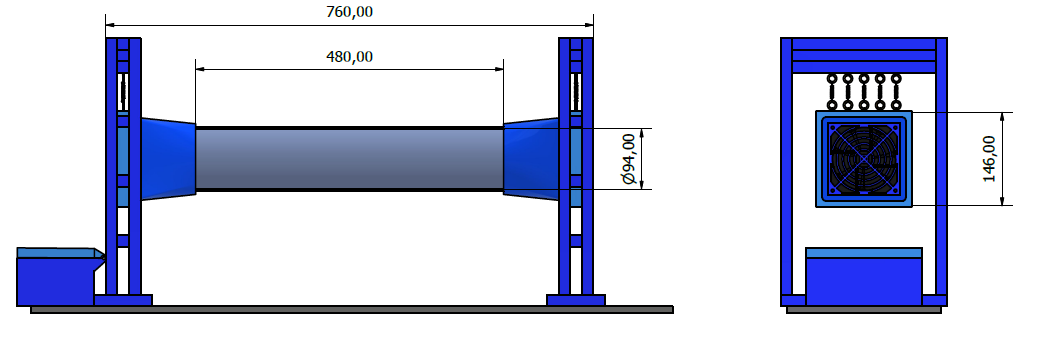
\includegraphics[width=0.8\linewidth]{images/dimen.png}
    \caption{Dimensiones generales del túnel de viento.}
    \label{fig:sim}
\end{figure}

\pagebreak

\begin{figure}[!ht]
    \centering
    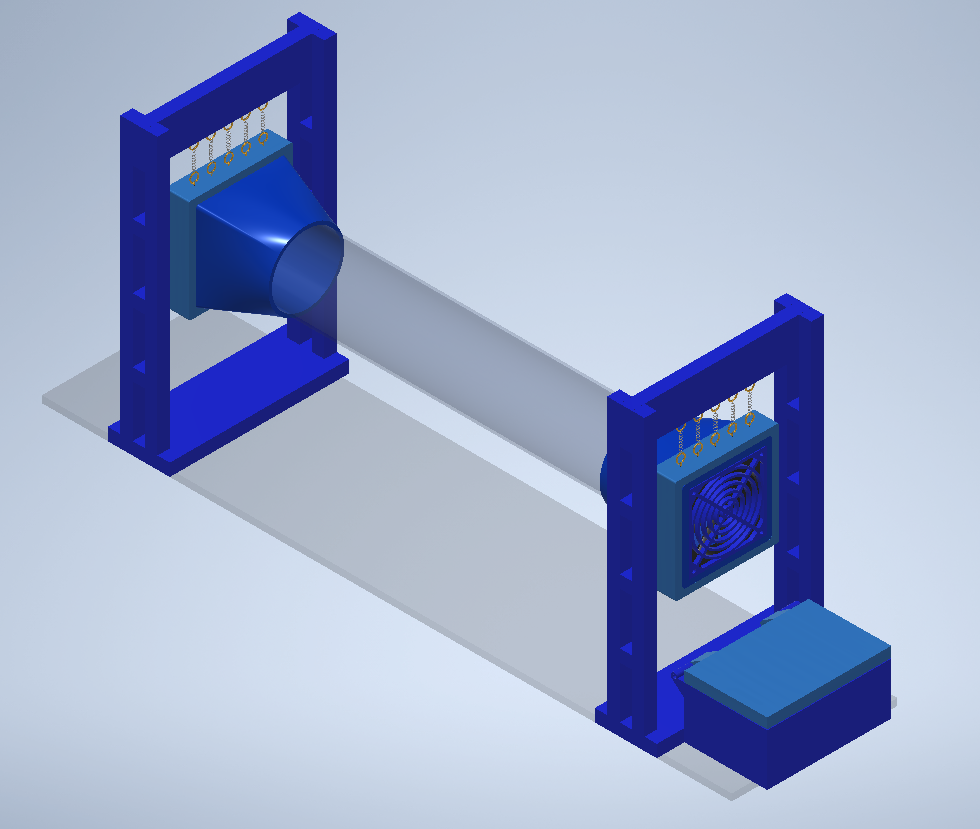
\includegraphics[width=0.5\linewidth]{images/exp.png}
    \caption{Vista isométrica del modelo CAD del dispositivo experimental.}
    \label{fig:cad_model}
\end{figure}

\begin{figure}[!ht]
    \centering
    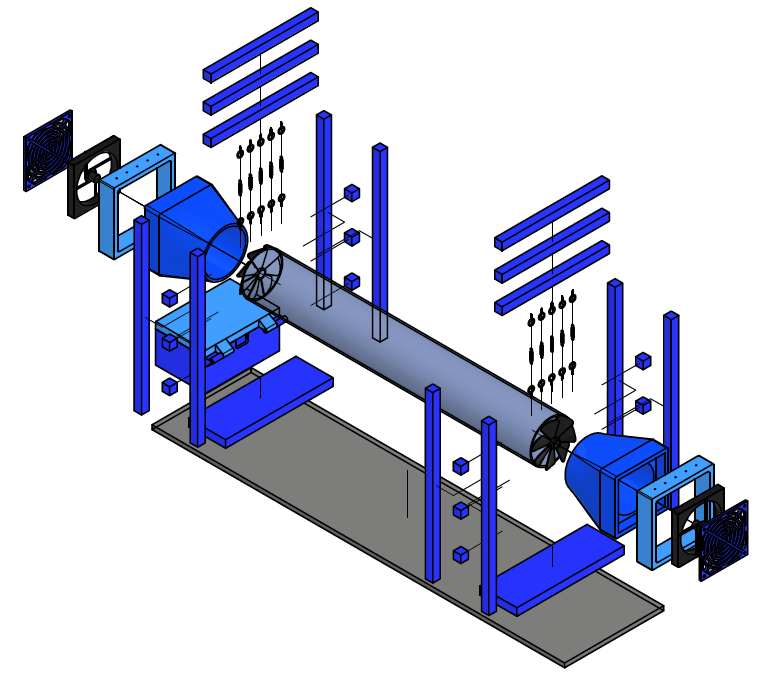
\includegraphics[width=0.5\linewidth]{images/explo.png}
    \caption{Vista explosionada del modelo CAD del dispositivo experimental.}
    \label{fig:explo}
\end{figure}

\subsection{Ventilador y Sistema de Control}
Se seleccionó un ventilador axial con capacidad de regular su velocidad mediante señal PWM. El ventilador, montado en la cámara de entrada, se sincroniza con el microcontrolador Arduino para variar las RPM (revoluciones por minuto) en función de los requerimientos del experimento y las pruebas de validación CFD. La transmisión de potencia y la robustez mecánica del montaje se verificaron para minimizar desbalances y vibraciones innecesarias.

\pagebreak
\section{Instrumentación y Disposición de Sensores}
\subsection{Sensores Seleccionados}
La selección de sensores descrita en el capítulo de Instrumentación respondió a la necesidad de medir variables eléctricas, mecánicas y térmicas. A continuación, se lista la disposición física de cada sensor en el túnel de viento:
\begin{itemize}
    \item \textbf{Sensor de Corriente ACS712:} Instalado en la línea de alimentación eléctrica del ventilador para medir el consumo de corriente.
    \item \textbf{Sensor de Voltaje PWM (0-25 V):} Conectado en paralelo al motor del ventilador para registrar la tensión aplicada y la modulación de ancho de pulso.
    \item \textbf{Sensor de Temperatura LM35:} Ubicado próximo al motor del ventilador para monitorear el sobrecalentamiento y la influencia de la velocidad de giro en la temperatura.
    \item \textbf{Cámara Térmica AMG8833:} Orientada hacia la carcasa del ventilador y las paredes del túnel para capturar un mapa térmico de la distribución del calor.
    \item \textbf{Acelerómetro MPU6050:} Montado en la base del ventilador para registrar vibraciones y movimientos provocados por desbalances en las aspas o resonancias del sistema.
    \item \textbf{Sensor de Flujo de Aire Indirecto (Anemómetro Calibrado):} Colocado dentro de la cámara de salida para medir la velocidad del flujo de aire.
\end{itemize}

La disposición de los sensores en el modelo experimental se detalla en la figura \ref{fig:sens}, y enumerados en la tabla \ref{tab:senso}.

\begin{figure}[!ht]
    \centering
    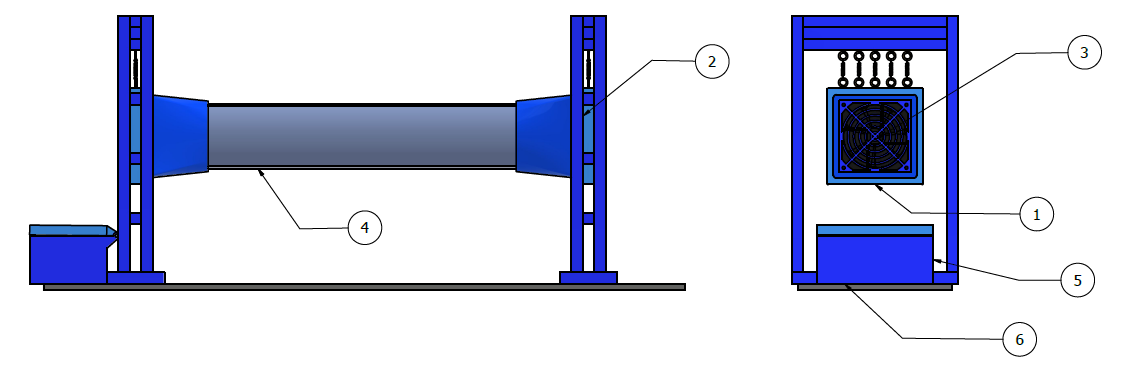
\includegraphics[width=0.8\linewidth]{images/sens.png}
    \caption{Esquema de disposición de los sensores.}
    \label{fig:sens}
\end{figure}

\begin{table}[H]
    \centering
    \caption{Listado de sensores utilizados.}
    \begin{tabular}{|c|l|l|}
    \hline
    \multicolumn{3}{|c|}{\textbf{Listado de sensores}} \\
    \hline
    \textbf{Elemento} & \textbf{Nombre}       & \textbf{Descripción}                          \\
    \hline
    1 & Acelerómetro      & Mide las vibraciones                       \\
    2 & Anemómetro        & Mide la velocidad de viento               \\
    3 & Termómetro        & Mide la temperatura del ventilador        \\
    4 & Cámara térmica    & Perfil de temperatura del ventilador      \\
    5 & Amperímetro       & Mide la corriente suministrada            \\
    6 & Voltímetro        & Mide el voltaje del ventilador            \\
    \hline
    \end{tabular}
    \label{tab:senso}
    \end{table}
    
\subsection{Integración con el Microcontrolador Arduino}
Todos los sensores se comunican con el microcontrolador Arduino a través de puertos analógicos o digitales, dependiendo de la naturaleza de la señal:
\begin{itemize}
    \item \textbf{ACS712 y Sensor de Voltaje PWM:} Conectados a las entradas analógicas para la lectura continua de la corriente y el voltaje.
    \item \textbf{LM35 y Anemómetro:} También acoplados a entradas analógicas; se utilizó un condensador de filtrado en el anemómetro para reducir el ruido.
    \item \textbf{MPU6050:} Comunicación digital I2C, que permite la transmisión simultánea de datos de acelerómetro y giroscopio.
    \item \textbf{AMG8833:} Comunicación digital I2C para la lectura matricial de valores de temperatura.
\end{itemize}

Se definieron tasas de muestreo específicas para cada sensor, equilibrando la precisión requerida con la capacidad de procesamiento. De esta manera, se evita la saturación en la transmisión de datos y se garantizan muestras representativas.

\section{Arquitectura de Adquisición y Procesamiento de Datos}
\subsection{Estructura General}
La lógica de adquisición y procesamiento de datos se compone de los siguientes elementos:
\begin{enumerate}
    \item \textbf{Microcontrolador Arduino:} Encargado de leer los sensores y controlar la velocidad del ventilador mediante señal PWM.
    \item \textbf{Servicio REST API:} Permite la interacción con la interfaz web y la base de datos, recibiendo peticiones para la configuración del ventilador o el inicio de la captura de datos.
    \item \textbf{Interfaz Web de Control:} Da acceso a los usuarios para ajustar la velocidad del ventilador, visualizar datos en tiempo real y seleccionar qué variables medir.
    \item \textbf{Base de Datos SQLite:} Se encarga de almacenar los datos de forma estructurada para su posterior análisis.
\end{enumerate}

\subsection{Programación del Sistema de Obtención de Datos}
En el microcontrolador Arduino se desarrolló un código modular, con las siguientes funciones principales:
\begin{itemize}
    \item \texttt{setup()}: Inicializa la comunicación con los sensores (I2C, puertos analógicos) y configura los pines de salida para la señal PWM.
    \item \texttt{loop()}: Ejecuta la rutina principal en la que se leen los valores de cada sensor, se calcula la media de las muestras durante un intervalo configurable y se envían los datos a través de la comunicación serial o Wi-Fi (dependiendo de la placa Arduino utilizada).
    \item \texttt{readSensors()}: Funciones individuales que retornan la lectura de corriente, voltaje, temperatura, vibración y flujo de aire.
    \item \texttt{setFanSpeed(value)}: Aplica la señal PWM para regular la velocidad de rotación del ventilador en función de un valor de consigna (0-255 en escalado Arduino o 0-100\%).
\end{itemize}

\section{Implementación de la REST API}
Para habilitar la comunicación entre Arduino y la aplicación web, se definió un servicio REST API (Representational State Transfer) ejecutado en una plataforma intermedia (por ejemplo, un servidor local o un \textit{single-board computer} con Linux). El servicio escucha peticiones HTTP (\texttt{GET}, \texttt{POST}) para:
\begin{itemize}
    \item \textbf{Configurar:} Cambiar la velocidad del ventilador o ajustar la frecuencia de muestreo de los sensores.
    \item \textbf{Iniciar/Detener la Lectura de Datos:} Gestionar los eventos de captura de información en el Arduino.
    \item \textbf{Obtener Datos:} Solicitar y recibir mediciones actualizadas en formato JSON, para ser almacenadas o visualizadas.
\end{itemize}

La conexión entre Arduino y este servicio puede realizarse de forma serial o inalámbrica (Wi-Fi o Bluetooth), dependiendo de la configuración elegida. El servicio REST API se programó en Python (utilizando el framework \texttt{Flask}), aunque pueden emplearse también entornos como Node.js o Java.

\section{Interfaz Web de Control y Selección de Datos}
\subsection{Diseño de la Interfaz}
La interfaz web (Fig.~\ref{fig:web}), accesible desde un navegador, proporciona una forma amigable de controlar el prototipo y visualizar la información en tiempo real. Sus secciones principales incluyen:
\begin{itemize}
    \item \textbf{Panel de Control de Velocidad:} Permite ajustar manualmente las RPM del ventilador o seleccionar modos automáticos predefinidos.
    \item \textbf{Panel de Datos en Tiempo Real:} Muestra gráficas de corriente, voltaje, temperatura, flujo de aire y vibración. Se utilizan librerías JavaScript como \texttt{Chart.js} o \texttt{D3.js} para la representación gráfica.
    \item \textbf{Selección de Variables a Medir:} El usuario define qué sensores deben estar activos y la frecuencia de muestreo para cada uno.
    \item \textbf{Historial de Lecturas:} Permite consultar y exportar datos pasados almacenados en la base de datos.
\end{itemize}

\begin{figure}[!ht]
    \centering
    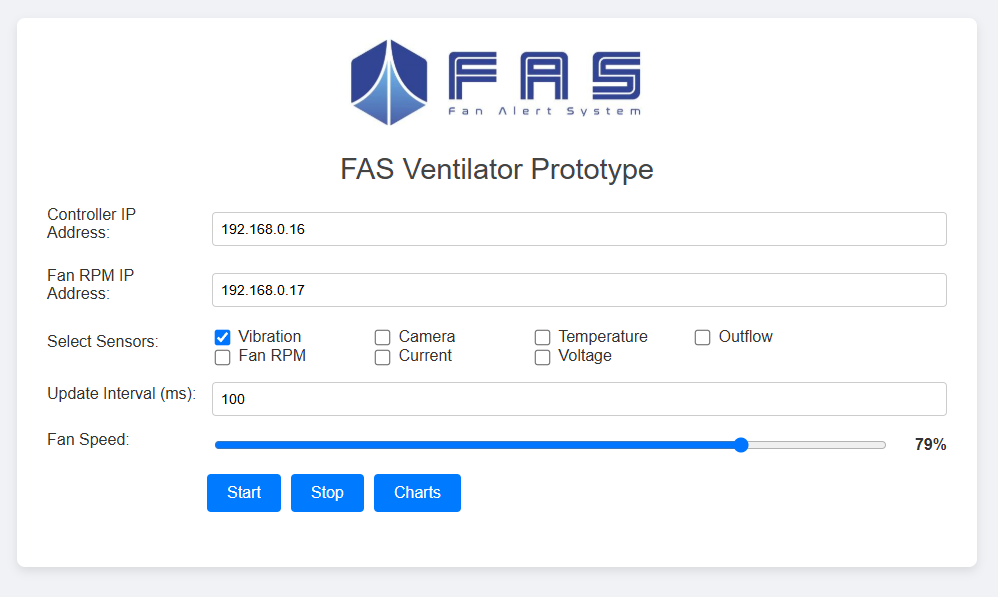
\includegraphics[width=0.8\linewidth]{images/web.png}
    \caption{Panel del control del dispositivo experimental.}
    \label{fig:web}
\end{figure}

\subsection{Interacción con la API}
La interfaz web se comunica con la API mediante peticiones \texttt{AJAX} (\texttt{GET} y \texttt{POST}), recibiendo datos en formato JSON. En cada consulta, el navegador interpreta la respuesta y actualiza dinámicamente la gráfica o los indicadores del panel de control.

\section{Almacenamiento de Datos en SQLite}
\subsection{Estructura de la Base de Datos}
Para el registro de la información se optó por SQLite, una base de datos liviana que no requiere un servidor dedicado, adecuada para prototipos y sistemas embebidos. La estructura contempla las siguientes tablas:

\begin{itemize}
    \item \texttt{measurements}: Almacena las lecturas de cada sensor. Los campos básicos incluyen:
    \begin{itemize}
        \item \texttt{id} (INTEGER, clave primaria autoincremental)
        \item \texttt{timestamp} (DATETIME)
        \item \texttt{sensor\_type} (TEXT) \textit{[p. ej. adxl345, amg8833, fanrpm, etc]}
        \item \texttt{value} (REAL)
    \end{itemize}
    
    \item \texttt{configurations}: Registra configuraciones de experimento, como la velocidad del ventilador, la frecuencia de muestreo y la duración de la captura.
    \begin{itemize}
        \item \texttt{id} (INTEGER, clave primaria autoincremental)
        \item \texttt{fan\_speed} (INTEGER)
        \item \texttt{sampling\_rate} (INTEGER)
        \item \texttt{date\_created} (DATETIME)
    \end{itemize}
\end{itemize}

\subsection{Inserción y Consulta de Datos}
Tras cada petición de lectura en el Arduino, la API recibe un paquete JSON con las mediciones, que posteriormente se insertan en la tabla \texttt{data}. Véase la figura~\ref{fig:table}.

\begin{figure}[!ht]
    \centering
    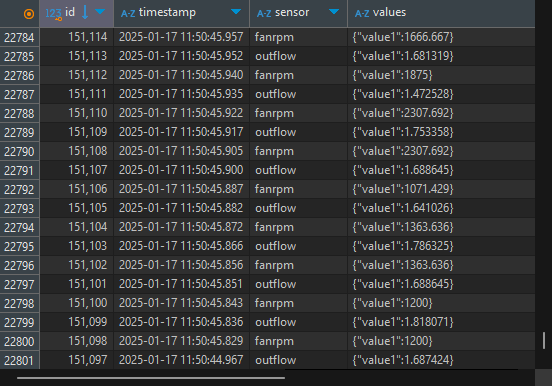
\includegraphics[width=0.5\linewidth]{images/table.png}
    \caption{Ejemplo de tabla de datos de sensores.}
    \label{fig:table}
\end{figure}

La consulta de datos se realiza directamente desde la base de datos, utilizando aplicaciones de gestión de base de datos para filtrar y exportar los datos según rangos de fechas, sensores y/o valores para su posterior análisis.

\newpage
\section{Simulación Computacional (CFD) en ANSYS}
\subsection{Preparación del Modelo CAD}
Para realizar la simulación CFD, se modeló la geometría del túnel de viento a escala en un software de diseño asistido por computadora (CAD). Se representó tanto la sección de entrada como la cámara principal, incluyendo la ubicación aproximada del ventilador. Este modelo 3D se exportó en un formato compatible (por ejemplo, \texttt{.igs} o \texttt{.step}) para ser importado posteriormente a ANSYS SpaceClaim (Fig.~\ref{fig:space}).

\begin{figure}[!ht]
    \centering
    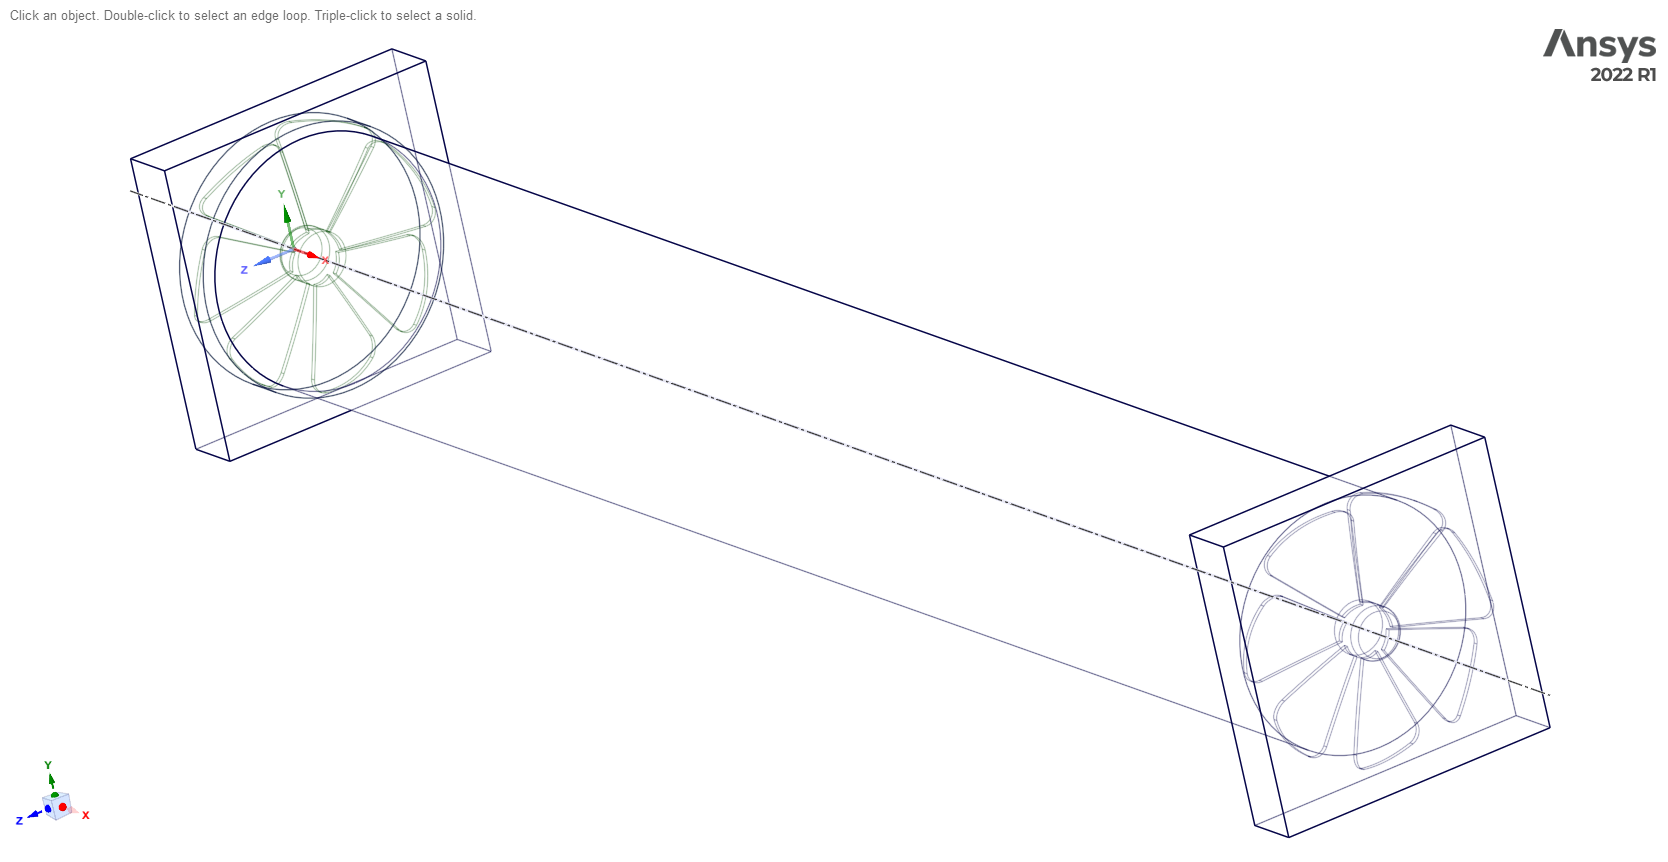
\includegraphics[width=0.8\linewidth]{images/space.png}
    \caption{Geometría del modelo en ANSYS SpaceClaim.}
    \label{fig:space}
\end{figure}

\newpage

\subsection{Configuración en ANSYS Fluent}
Una vez importada la geometría en ANSYS, se procedió a:
\begin{enumerate}
    \item \textbf{Creación de la malla:} Se generó una malla policéntrica compuesta por hexaedros y tetraedros, dependiendo de la complejidad de las cavidades. Se prestó especial atención a la región próxima al ventilador y a las zonas donde se esperaba mayor gradiente de velocidad. (Fig.~\ref{fig:mesh})
    \item \textbf{Selección del modelo de turbulencia:} Se optó por el modelo \texttt{k-$\epsilon$} estándar, apropiado para flujos internos con niveles moderados de turbulencia. 
    \item \textbf{Condiciones de contorno:} Se definió la entrada y salida de aire como una condición de velocidad o caudal (dependiendo del escenario). Se establecieron superficies sólidas con la pared del túnel y la carcasa del ventilador. (El flujo de aire se da por la diferencia de presión generada por la rotación del ventilador). En la figura \ref{fig:borde} se pueden apreciar las condiciones de contorno de manera gráfica. En azul la entrada de aire, en rojo la salida de aire y en amarillo la interfaz de la zona de rotación del ventilador.
    \item \textbf{Propiedades del fluido:} Se consideró aire como fluido ideal, con densidad aproximada de 1.225 kg/m$^3$ y viscosidad de $1.8 \times 10^{-5}$ Pa·s, a temperatura ambiente.
    \item \textbf{Configuración de la rotación del ventilador:} Para simular el efecto del ventilador, se definió una zona de rotación (\textit{rotating domain}) a una velocidad de rotación configurable según los experimentos.
\end{enumerate}

\begin{figure}[!ht]
    \centering
    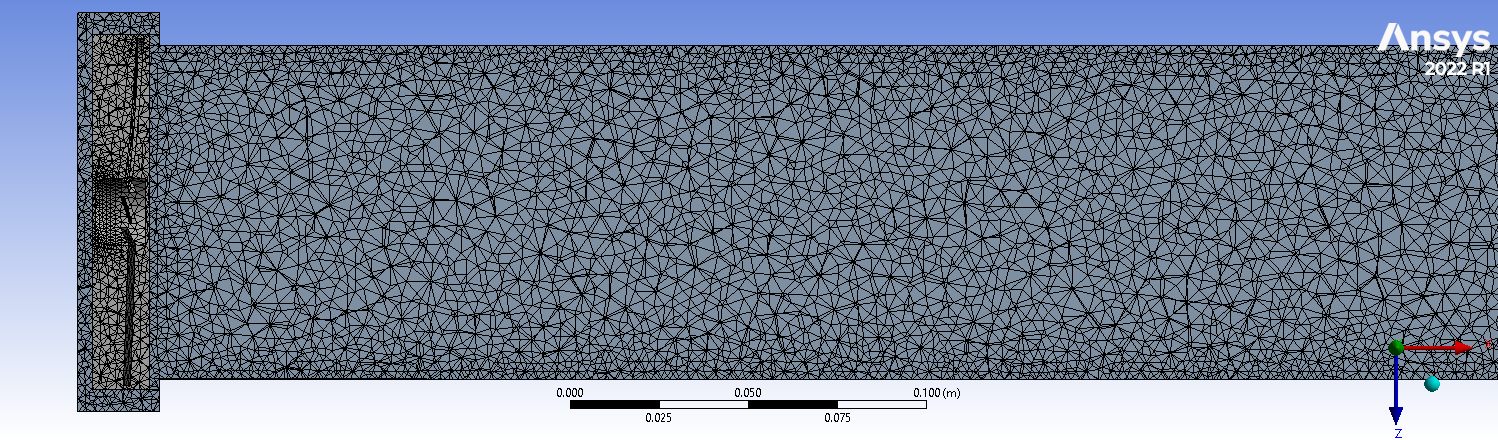
\includegraphics[width=0.7\linewidth]{images/mesh.png}
    \caption{Mallado realizado en ANSYS.}
    \label{fig:mesh}
\end{figure}

\begin{figure}[!ht]
    \centering
    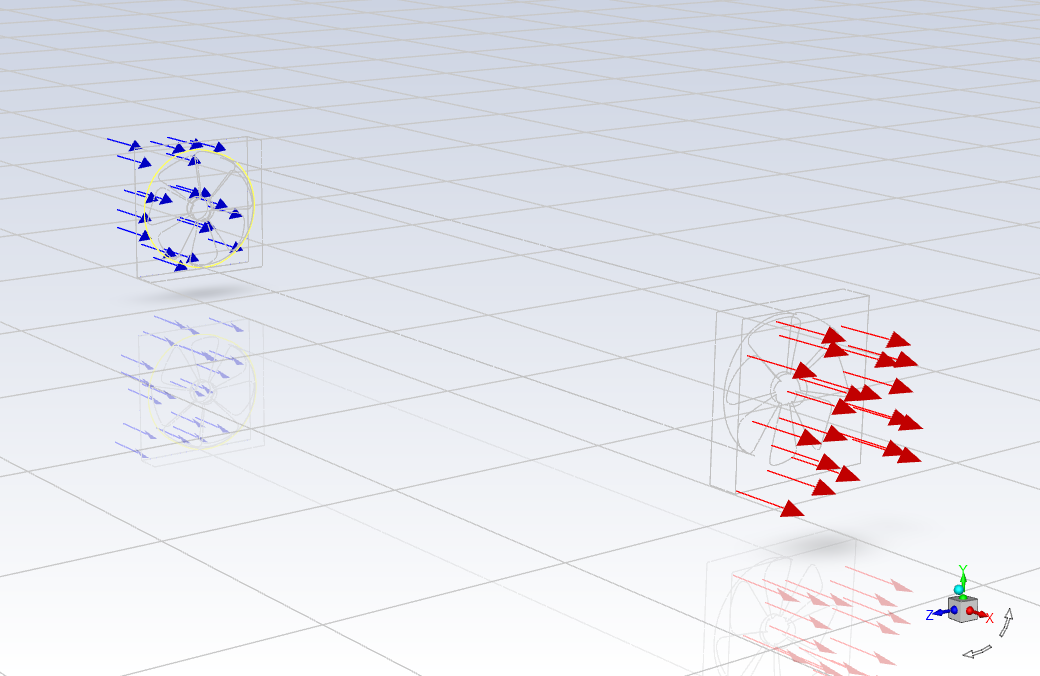
\includegraphics[width=0.7\linewidth]{images/borde.png}
    \caption{Condiciones de borde aplicadas en ANSYS Fluent.}
    \label{fig:borde}
\end{figure}

\subsection{Cálculo y Convergencia}
Se seleccionó un esquema de discretización \textit{semi-implicit} y un método de acoplamiento presión-velocidad (SIMPLE o SIMPLER), ajustando el número de iteraciones hasta alcanzar convergencia (generalmente cuando los residuos de velocidad, presión y turbulencia descendieron a un valor menor a $10^{-4}$). El cálculo se realizó en iteraciones sucesivas, monitoreando parámetros de interés como la velocidad promedio en la sección de salida y la presión en la región del ventilador.



\subsection{Obtención de Resultados}
Tras la convergencia, se post-procesaron los resultados para extraer.
\begin{itemize}
    \item \textbf{Distribución de velocidades:} Campos vectoriales y escalas de magnitud de velocidad en el interior del túnel.
    \item \textbf{Presiones estática y dinámica:} Perfiles a lo largo de la sección principal, útiles para determinar pérdidas de carga.
    \item \textbf{Líneas de corriente (streamlines):} Visualización del patrón de flujo e identificación de zonas de recirculación.
    \item \textbf{Distribución de temperatura (opcional):} En caso de habilitar transferencia de calor para comparar con datos de la cámara térmica.
\end{itemize}

\section{Validación del Modelo CFD mediante Comparación de Datos}
\subsection{Diseño de las Pruebas de Validación}
Para validar el modelo numérico se definieron ensayos experimentales con el túnel de viento a distintas velocidades del ventilador (en un rango de 833-4200 RPM). Durante cada ensayo:
\begin{itemize}
    \item Se midió el consumo de corriente y voltaje del motor para relacionarlo con la potencia.
    \item Se registró la velocidad del flujo de aire en varios puntos de la cámara principal mediante el sensor de flujo calibrado.
    \item Se monitorearon vibraciones y temperaturas, en busca de correlaciones con las distribuciones de velocidad simuladas.
\end{itemize}

\subsection{Comparación Cualitativa y Cuantitativa}
\begin{enumerate}
    \item \textbf{Comparación cualitativa:} Se inspeccionaron visualmente las líneas de flujo y zonas de recirculación detectadas en la simulación, contrastándolas con el comportamiento real observado (por ejemplo, con humo trazador o patrones de polvo muy ligero en el túnel).
    \item \textbf{Comparación cuantitativa:} Se emplearon estadísticos como el \textit{error porcentual medio} (MAPE) o la diferencia absoluta promedio entre las velocidades simuladas y las medidas por el anemómetro. 

    \begin{equation}
    \text{Error\%} = \frac{\lvert v_{\text{sim}} - v_{\text{exp}} \rvert}{v_{\text{exp}}} \times 100
    \end{equation}

    Se establecieron límites de aceptación basados en la precisión de los sensores y la complejidad del fenómeno (un error menor al 10\% se consideró razonable para este tipo de prototipo).
\end{enumerate}

\subsection{Ajustes y Retroalimentación}
En caso de observar discrepancias mayores a las esperadas, se realizaron ajustes en el modelo CFD:
\begin{itemize}
    \item Refinar la malla en zonas críticas y aumentar el número de capas en la región de la capa límite.
    \item Modificar el modelo de turbulencia o los valores de parámetros en \texttt{k-$\epsilon$}.
    \item Incluir efectos de compresibilidad o calor, si fuera necesario.
\end{itemize}

Tras cada ajuste, se repitió el proceso de simulación y validación, iterando hasta lograr un nivel satisfactorio de concordancia entre datos experimentales y simulados.

%%%%%%%%%%%%%%%%%%%%%%%%%%%%%%%%%%%%%%%%%%%%%%%%%%%%%%%%%%%%%%%
\section{Evaluación Cualitativa de los Datos}

Este apartado se centra exclusivamente en la revisión y análisis cualitativo de los datos disponibles, con el propósito de determinar si, en un futuro, podrían emplearse para entrenar un modelo de mantenimiento predictivo. A continuación, se describe la metodología básica para dicha evaluación.

\subsection{Recopilación y Organización de Datos}
En primer lugar, se reúnen y clasifican los datos provenientes de:
\begin{enumerate}
    \item \textbf{Prototipo Experimental:} Incluye mediciones de RPM, velocidad del viento, vibraciones y temperaturas, así como parámetros eléctricos (corriente y voltaje).
    \item \textbf{Simulación CFD:} Ofrece distribuciones de velocidad, gradientes de presión y patrones de flujo bajo diferentes regímenes de rotación del ventilador.
\end{enumerate}
La información se integra en un único repositorio o formato que permita su revisión conjunta (tablas de datos, hojas de cálculo, etc.).

\subsection{Análisis Exploratorio}
Tras la unificación de los datos, se realiza un examen cualitativo con el fin de:
\begin{itemize}
    \item \textbf{Visualizar Tendencias:} Inspeccionar, mediante gráficas o listados, cómo varían las RPM o la velocidad del viento en distintos escenarios de operación o configuraciones de la simulación.
    \item \textbf{Comparar Fuentes de Datos:} Identificar posibles divergencias entre las lecturas experimentales y los resultados simulados para detectar comportamientos atípicos o inconsistencias.
    \item \textbf{Relaciones Básicas:} Explorar, de manera cualitativa, si un incremento en las RPM coincide con mayores vibraciones o si cambios en la velocidad del viento repercuten de forma notoria en la corriente consumida.
\end{itemize}

\subsection{Formulación de Observaciones Cualitativas}
Con base en las tendencias y comparaciones realizadas, se elaboran conclusiones preliminares que describen de forma no cuantificada:
\begin{itemize}
    \item \textbf{Patrones de Operación:} Zonas de funcionamiento estable versus rangos en los que se observan irregularidades como altos picos de vibración o sobrecalentamiento.
    \item \textbf{Semejanzas y Discrepancias:} Grado de concordancia entre los valores medidos y las predicciones de la simulación, indicando si ésta refleja adecuadamente la realidad o si existen supuestos simplificados.
    \item \textbf{Indicadores de Posible Falla:} Apreciaciones sobre signos potenciales de desgaste en el ventilador (p.ej., aumento sostenido de temperatura o vibraciones no esperadas).
\end{itemize}

\subsection{Conclusión y Viabilidad para un Futuro Modelo}
Finalmente, se emite un juicio cualitativo acerca de si los datos recabados presentan la variedad y consistencia necesarias para, en el futuro, generar un modelo de mantenimiento predictivo. En caso afirmativo, se sugiere profundizar en análisis estadísticos o incluir más variables de interés. Si no se detecta información suficiente, se recomienda ampliar la toma de datos o refinar la metodología de medición y simulación.

\noindent
Este proceso de evaluación cualitativa constituye un punto de partida para determinar de manera inicial la factibilidad de desarrollar herramientas predictivas a partir de los datos de RPM, velocidad de viento y demás variables monitorizadas tanto en la prueba experimental como en la simulación.


%%%%%%%%%%%%%%%%%%%%%%%%%%%%%%%%%%%%%%%%%%%%%%%%%%%%%%%%%%%%%%%%
\section{Flujo de Trabajo}
En términos generales, el flujo de trabajo para realizar una prueba experimental y su validación CFD es:
\begin{enumerate}
    \item \textbf{Configuración de la prueba:} El usuario accede a la interfaz web y ajusta la velocidad del ventilador y la lista de sensores a monitorear.
    \item \textbf{Adquisición de datos:} La interfaz web envía la configuración a la API y el Arduino comienza a leer los sensores, transmitiendo datos que se almacenan en SQLite.
    \item \textbf{Generación del modelo CFD:} Se prepara la geometría y la malla en ANSYS, aplicando condiciones de contorno que emulen las condiciones del prototipo (velocidad, caudal, presión, etc.).
    \item \textbf{Ejecución de la simulación:} Se corre el solver CFD y se monitorean los residuos hasta alcanzar la convergencia.
    \item \textbf{Post-procesado y extracción de datos:} Se obtienen campos de velocidad, presión, temperatura, etc. 
    \item \textbf{Comparación y validación:} Se contrasta la información simulada con las mediciones experimentales de velocidad, corriente, vibración y temperatura.
    \item \textbf{Ajuste o refinamiento:} Se corrige la malla o se varían los parámetros del modelo CFD para reducir diferencias con la realidad.
    \item \textbf{Evaluación cualitativa de datos:} Se analizan las fuentes y calidad de datos para evaluar el desarrollo de modelos de mantenimiento predictivos basados en machine learning.
\end{enumerate}

\pagebreak
\section{Resumen de la Metodología}
La metodología propuesta integra el diseño de un prototipo físico de túnel de viento a escala con un sistema automatizado de adquisición de datos que comunica los sensores con una API REST y una interfaz web interactiva. El almacenamiento en \texttt{SQLite} permite un acceso rápido y versátil a las mediciones, facilitando la comparación entre datos experimentales y simulaciones CFD en ANSYS. La validación se establece al correlacionar los valores de velocidad, temperatura y vibración medidos con los campos numéricos simulados, permitiendo ajustar el modelo computacional hasta lograr concordancias aceptables. Esta arquitectura modular es escalable y puede adaptarse para futuras extensiones, como la incorporación de algoritmos de machine learning o la migración a sistemas de mayor complejidad en escenarios mineros reales.

\chapter{Resultados}

Este capítulo presenta los resultados obtenidos tras la implementación de la plataforma de control y adquisición de datos, el almacenamiento de información en la base de datos SQLite y el análisis de la simulación CFD. Finalmente, se exponen los valores comparativos de velocidad de flujo de aire medidos y simulados a diferentes velocidades de giro (RPM) del ventilador.

\section{Plataforma de Control y Adquisición de Datos}
\subsection{Interfaz Web de Control}
La interfaz web desarrollada permitió a los usuarios configurar en tiempo real la velocidad del ventilador, seleccionar los sensores a monitorear y observar la evolución de las variables medidas. Como se muestra en la Figura \ref{fig:ui_plataforma}, la pantalla principal incluyó:
\begin{itemize}
    \item Un \textbf{panel de control de velocidad}, donde el operador ajustó manualmente las RPM o activó modos de operación predefinidos.
    \item Un \textbf{panel de visualización en tiempo real}, con gráficas actualizadas de corriente, voltaje, temperatura, flujo de aire y vibración. Se utilizaron librerías de JavaScript para la representación dinámica de los datos.
    \item Un \textbf{menú de configuración}, que permitía definir la frecuencia de muestreo por sensor y activar/desactivar la adquisición de cada uno.
\end{itemize}

\begin{figure}[htbp]
    \centering
    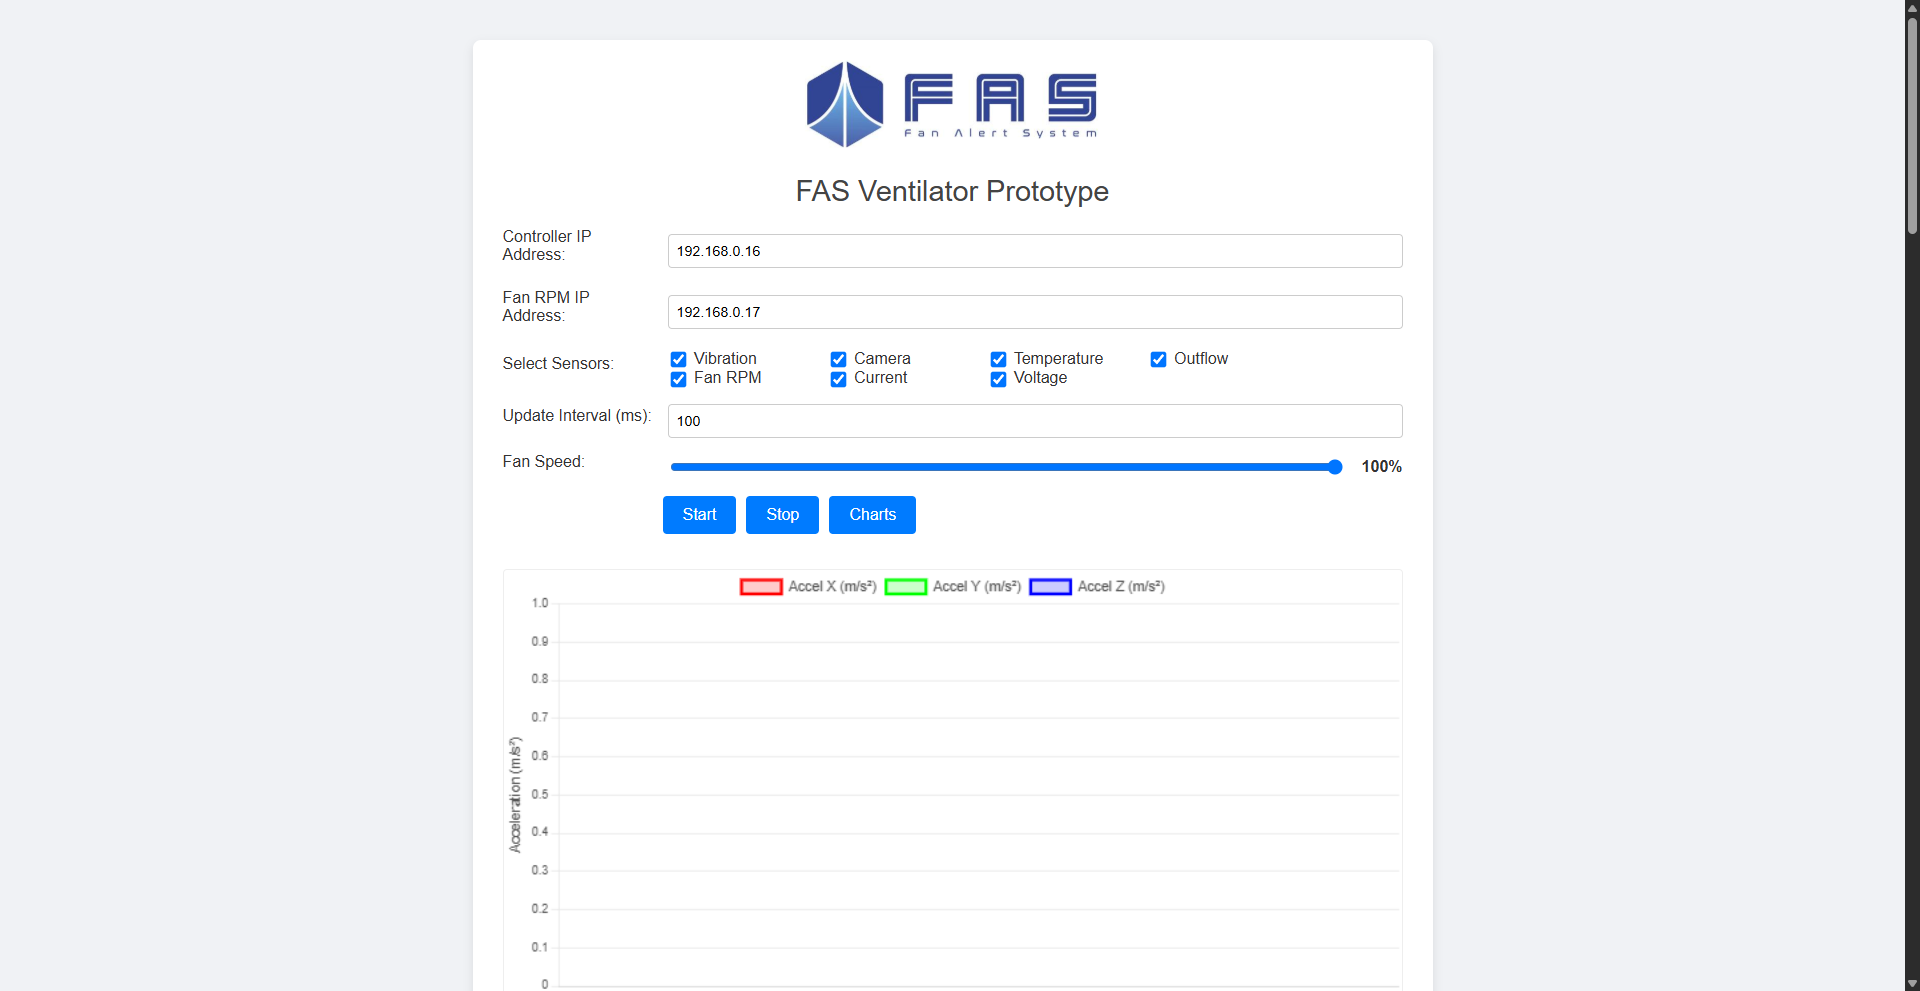
\includegraphics[width=0.75\textwidth]{images/webb.png}
    \caption{Ejemplo ilustrativo de la interfaz web de control y visualización.}
    \label{fig:ui_plataforma}
\end{figure}

\subsection{Configuración de Pruebas}
Para los ensayos de validación, se seleccionaron tres puntos de operación del ventilador: 833 RPM, 2500 RPM y 4200 RPM. En cada caso, el sistema registró continuamente las mediciones de los sensores, almacenándolas con sus marcas de tiempo. La interfaz mostró en tiempo real la evolución de las variables, lo que permitió ajustar la estrategia de medición si se detectaban anomalías o inestabilidades.

\section{Almacenamiento en Base de Datos SQLite}
\subsection{Estructura y Persistencia de Datos}
El sistema de adquisición envió los datos al servicio REST API, que posteriormente realizó la inserción de registros en la base de datos SQLite. La Tabla \ref{tab:tabla_measurements} describe la estructura principal utilizada para guardar las mediciones.

\begin{table}[htbp]
    \centering
    \caption{Estructura simplificada de la tabla \texttt{measurements} en SQLite.}
    \label{tab:tabla_measurements}
    \begin{tabular}{l l l}
    \toprule
    \textbf{Campo} & \textbf{Tipo de dato} & \textbf{Descripción}\\
    \midrule
    id & INTEGER & Clave primaria autoincremental \\
    timestamp & DATETIME & Marca de tiempo de la medición \\
    sensor\_type & TEXT & Tipo de sensor (p.ej., \textit{current}, \textit{temperature}) \\
    value & REAL & Valor medido \\
    \bottomrule
    \end{tabular}
\end{table}

Durante cada prueba, se registraron en promedio entre 400 y 600 muestras por minuto, dependiendo de la frecuencia de muestreo definida. Este volumen de datos permitió contar con información suficiente para un análisis estadístico representativo, a la vez que la ligereza de SQLite resultó adecuada para un prototipo de laboratorio.

\subsection{Consulta y Exportación de Información}
La interfaz web proporcionó consultas con filtros de fecha, tipo de sensor y rango de valores. Asimismo, en las sesiones de validación se generaron exportaciones automáticas en formato CSV, que luego sirvieron para procesar la información en hojas de cálculo o software estadístico. De este modo, se facilitó la comparación directa con los resultados numéricos de la simulación.

\newpage
\section{Resultados de la Simulación CFD}
\subsection{Configuración del Modelo Computacional}
La geometría del túnel se importó a ANSYS, donde se creó una malla combinada (hex-dominante en las regiones de flujo principal y tetraedros en cavidades complejas). Para cada simulación se asignó un número de RPM al ventilador (833, 2500 o 4200 RPM) a través de una zona de rotación (\textit{rotating domain}). Las condiciones de contorno principales fueron:
\begin{itemize}
    \item \textbf{Entrada de aire}: Presión ambiente.
    \item \textbf{Salida}: Presión abierta (0 Pa de referencia).
    \item \textbf{Paredes del túnel}: Condición de no deslizamiento (\textit{no-slip}).
\end{itemize}

El modelo de turbulencia utilizado fue \texttt{k-$\epsilon$} estándar, con discretización de segundo orden para ecuaciones de momento. La convergencia se obtuvo cuando los residuos numéricos se ubicaron por debajo de $10^{-4}$ y las variables clave (velocidad media en la salida, presión estática en la región del ventilador) estabilizaron sus valores.

%%%%%%%%%%%%%%%%%%%%%%%%%%%%%%%%%%%%%%%%%%%%%%%%%%%%%%%%%%%%%%%%%%
\subsection{Cálculo y convergencia}
Se muestran los gráficos de convergencia para los casos simulados a condiciones operacionales de 833 RPM, 2500 RPM y 4200 RPM (Fig. \ref{fig:res1}-\ref{fig:res3}).

\begin{figure}[!ht]
    \centering
    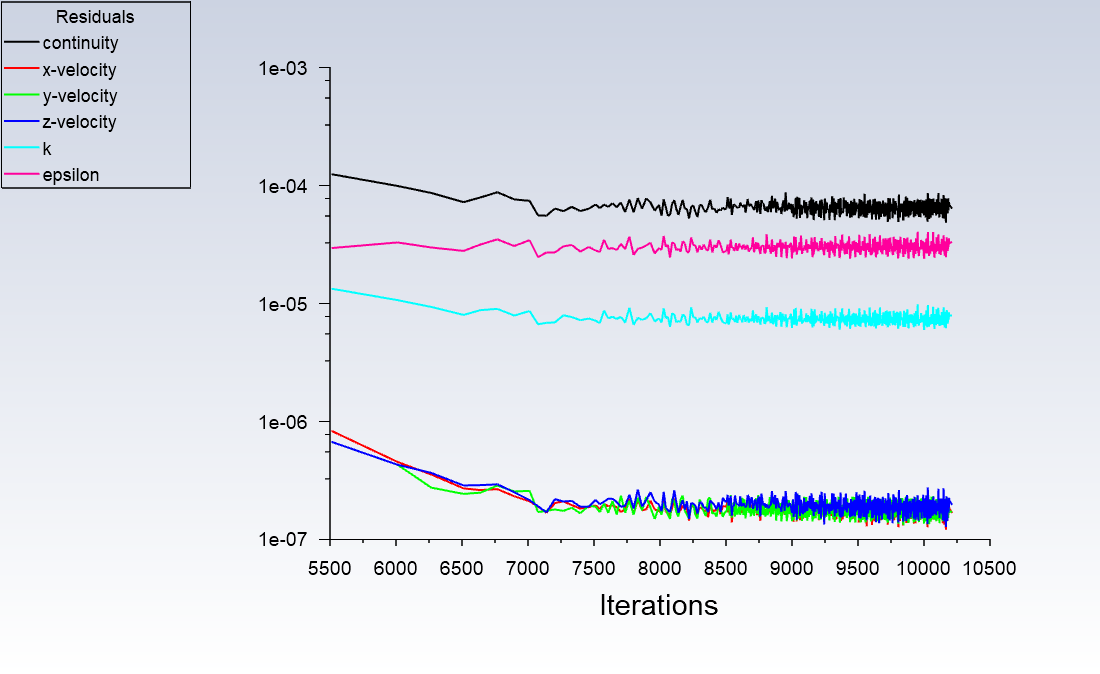
\includegraphics[width=0.7\linewidth]{images/res1.png}
    \caption{Gráfico de convergencia para 833 RPM.}
    \label{fig:res1}
\end{figure}

\pagebreak

\begin{figure}[!ht]
    \centering
    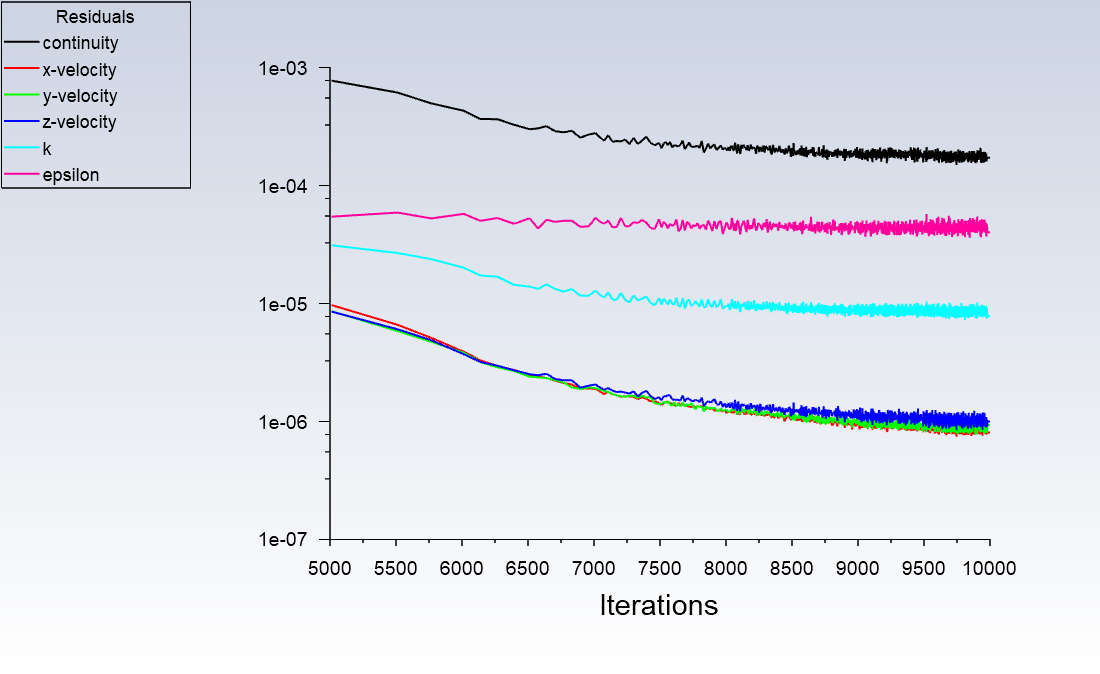
\includegraphics[width=0.7\linewidth]{images/res2.png}
    \caption{Gráfico de convergencia para 2500 RPM.}
    \label{fig:res2}
\end{figure}

\begin{figure}[!ht]
    \centering
    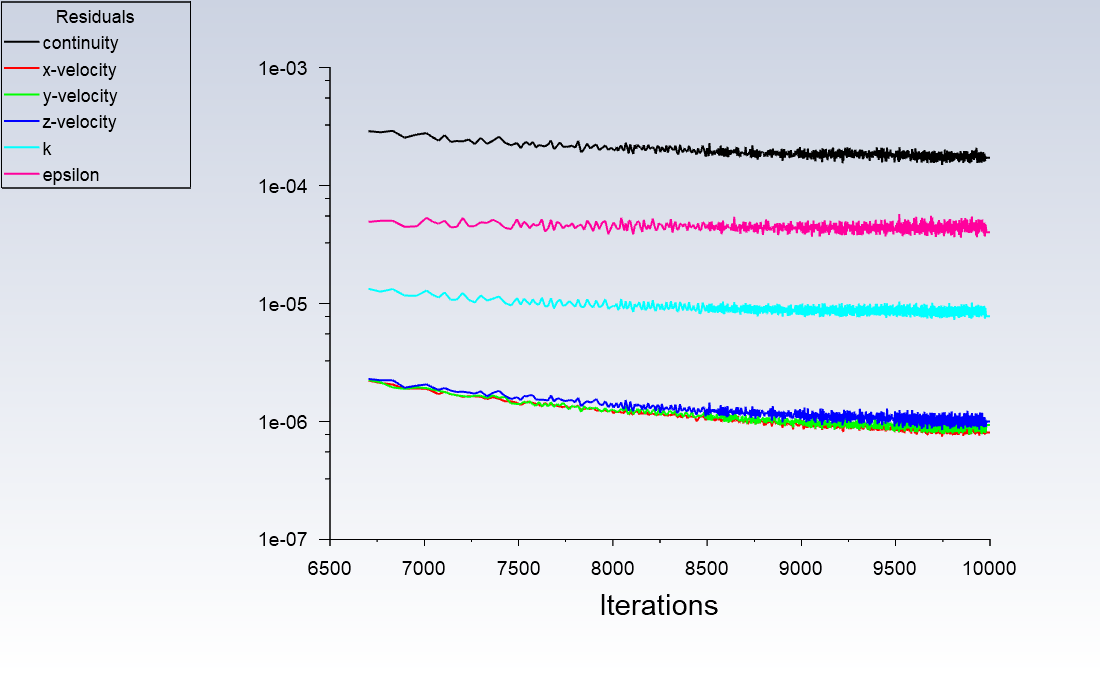
\includegraphics[width=0.7\linewidth]{images/res3.png}
    \caption{Gráfico de convergencia para 4200 RPM.}
    \label{fig:res3}
\end{figure}

Se puede notar que se alcanza la condición de convergencia en alrededor de 7000 a 9000 iteraciones.

%%%%%%%%%%%%%%%%%%%%%%%%%%%%%%%%%%%%%%%%%%%%%%%%%%%%%%%%%%%%%%%%%%%%
\newpage
\subsection{Distribución de velocidades}
La figuras \ref{fig:vel1}-\ref{fig:vel3} muestran los contornos de velocidad simulados para los casos considerados. Se aprecia que la región próxima a las aspas del ventilador presenta las mayores velocidades, que tienden a estabilizarse a medida que el flujo avanza hacia la cámara principal.

\begin{figure}[ht!]
    \centering
    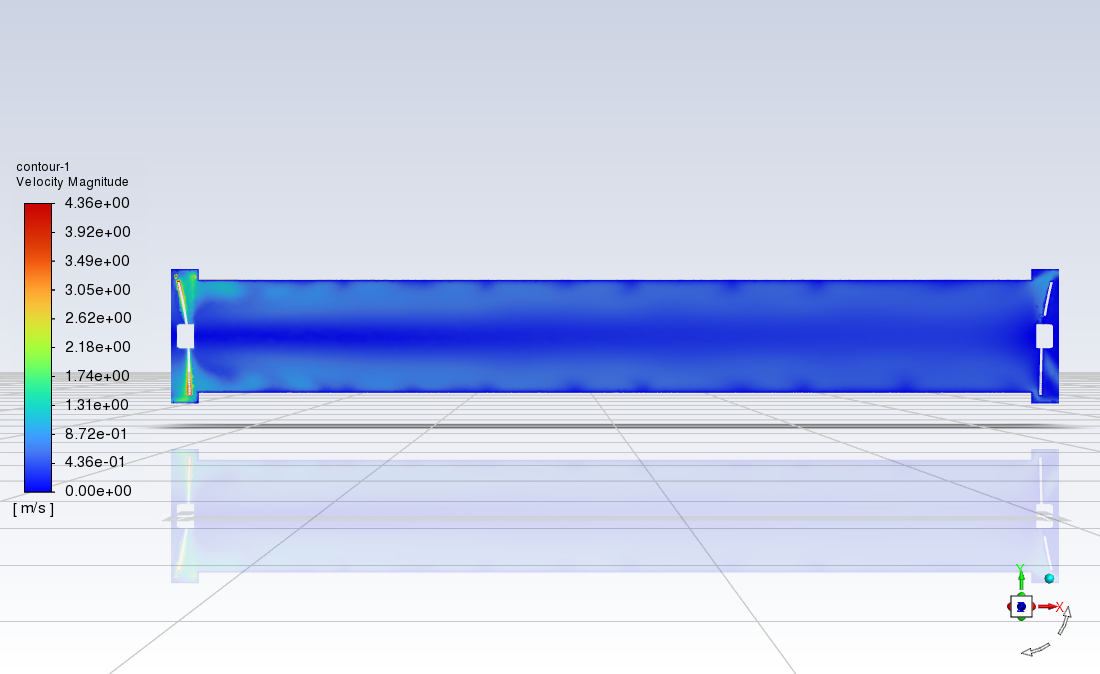
\includegraphics[width=0.9\textwidth]{images/vel1.png}
    \caption{Contornos de velocidad simulados (m/s) en el plano central del túnel para 833 RPM.}
    \label{fig:vel1}
\end{figure}

\begin{figure}[ht!]
    \centering
    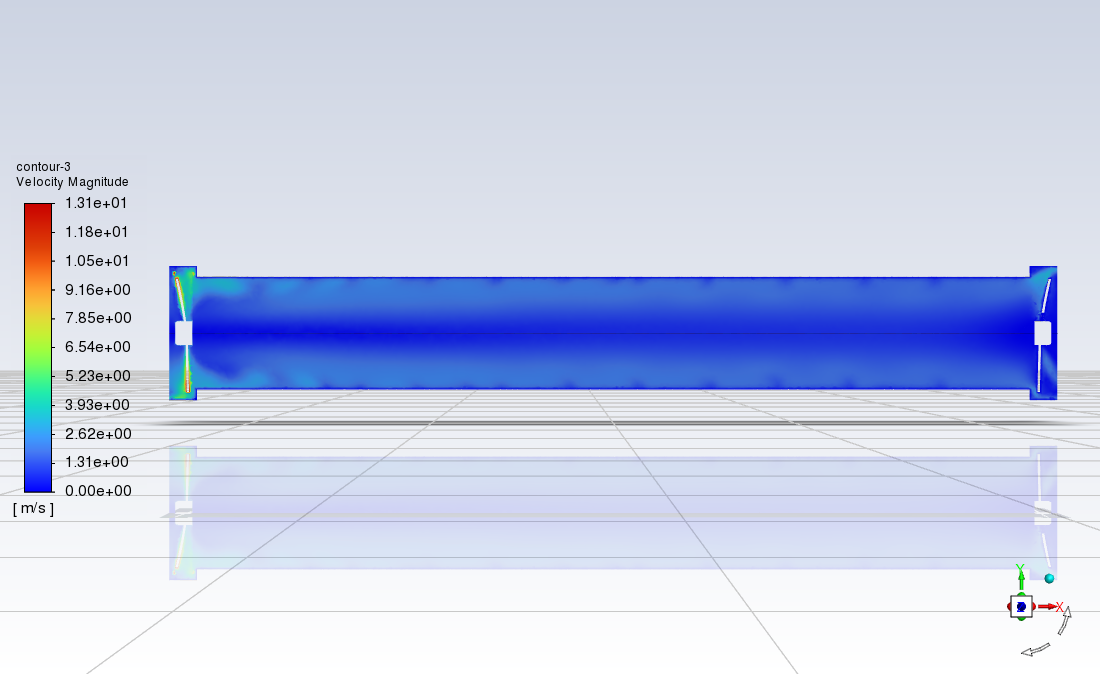
\includegraphics[width=0.9\textwidth]{images/vel2.png}
    \caption{Contornos de velocidad simulados (m/s) en el plano central del túnel para 2500 RPM.}
    \label{fig:vel2}
\end{figure}

\pagebreak

\begin{figure}[ht!]
    \centering
    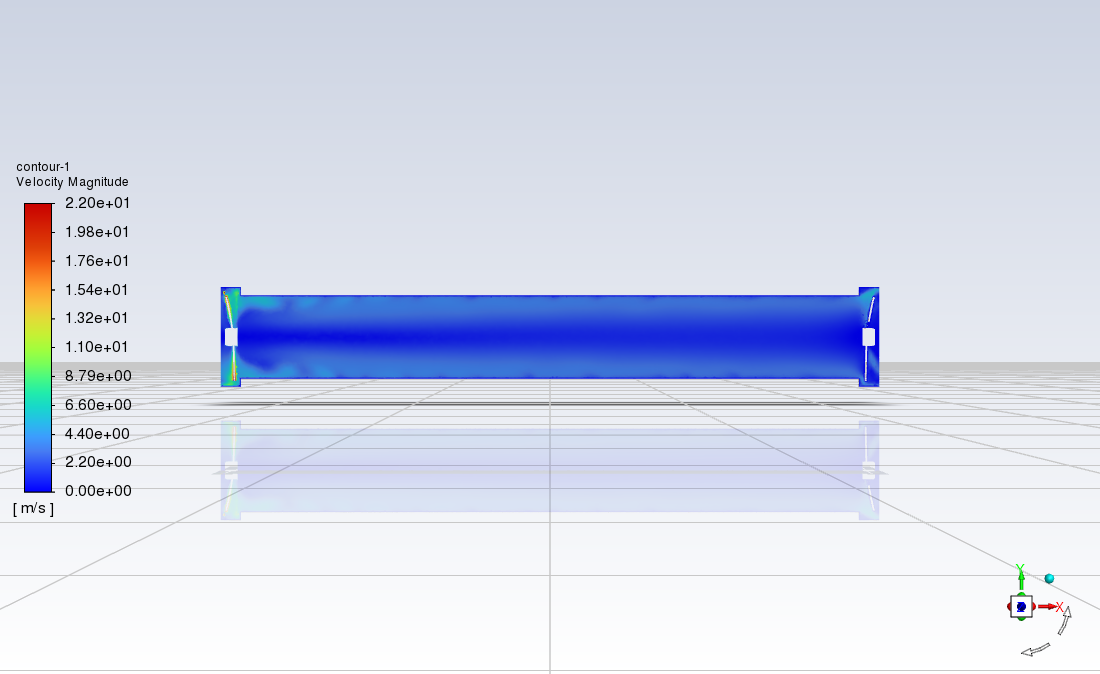
\includegraphics[width=0.9\textwidth]{images/vel3.png}
    \caption{Contornos de velocidad simulados (m/s) en el plano central del túnel para 4200 RPM.}
    \label{fig:vel3}
\end{figure}

En el plano transversal, se evidenciaron zonas de recirculación en las esquinas del conducto, especialmente a bajas RPM, lo cual concuerda con observaciones experimentales de zonas de velocidad reducida.

%%%%%%%%%%%%%%%%%%%%%%%%%%%%%%%%%%%%%%%%%%%%%%%%%%%%%%%%%%%%%%
\pagebreak
\subsection{Presiones estáticas y dinámicas}

En las figuras \ref{fig:sta1}-\ref{fig:sta3} se muestran los mapas de presión estática para los casos simulados.

\begin{figure}[!ht]
    \centering
    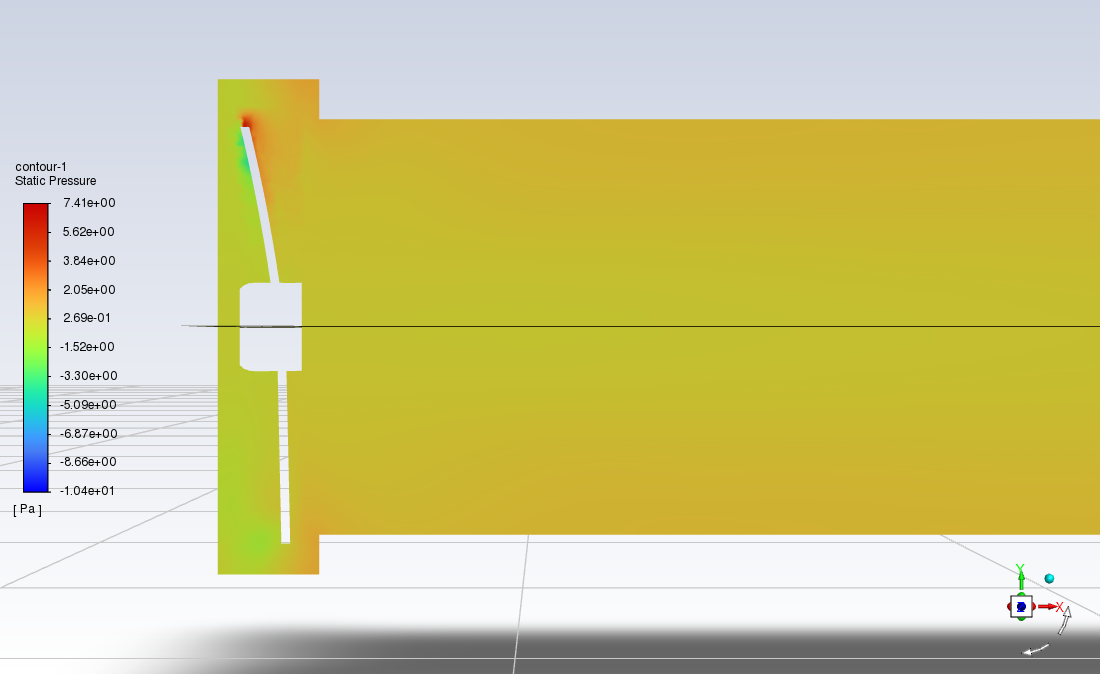
\includegraphics[width=0.6\textwidth]{images/sta1.png}
    \caption{Mapa de presión estática para 833 RPM.}
    \label{fig:sta1}
\end{figure}

\begin{figure}[!ht]
    \centering
    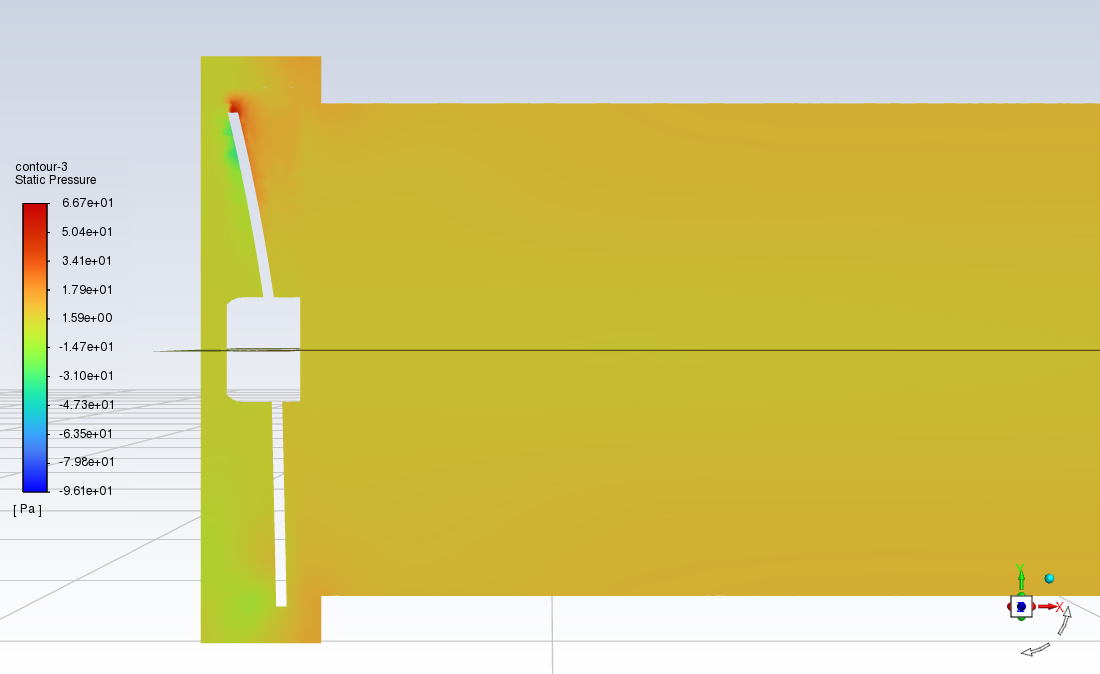
\includegraphics[width=0.6\textwidth]{images/sta2.png}
    \caption{Mapa de presión estática para 2500 RPM.}
    \label{fig:sta2}
\end{figure}

\begin{figure}[!ht]
    \centering
    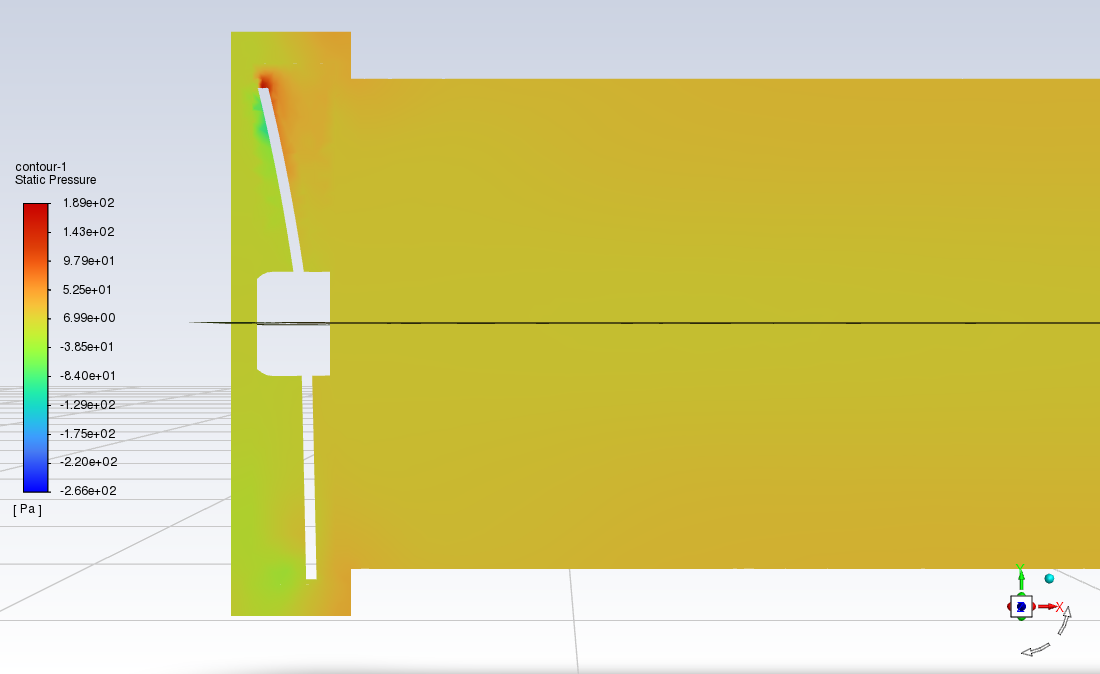
\includegraphics[width=0.6\textwidth]{images/sta3.png}
    \caption{Mapa de presión estática para 4200 RPM.}
    \label{fig:sta3}
\end{figure}

\pagebreak
En las figuras \ref{fig:dyn1}-\ref{fig:dyn3} se muestran los mapas de presión dinámica para los casos.

\begin{figure}[!ht]
    \centering
    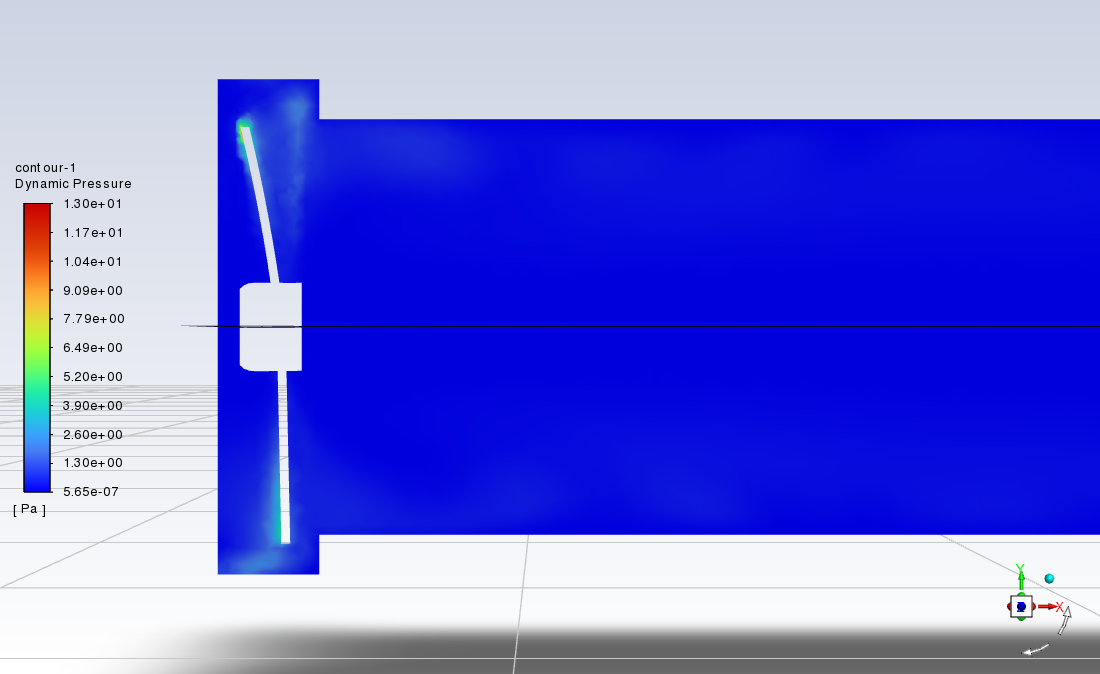
\includegraphics[width=0.6\textwidth]{images/dyn1.png}
    \caption{Mapa de presión dinámica para 833 RPM.}
    \label{fig:dyn1}
\end{figure}

\begin{figure}[!ht]
    \centering
    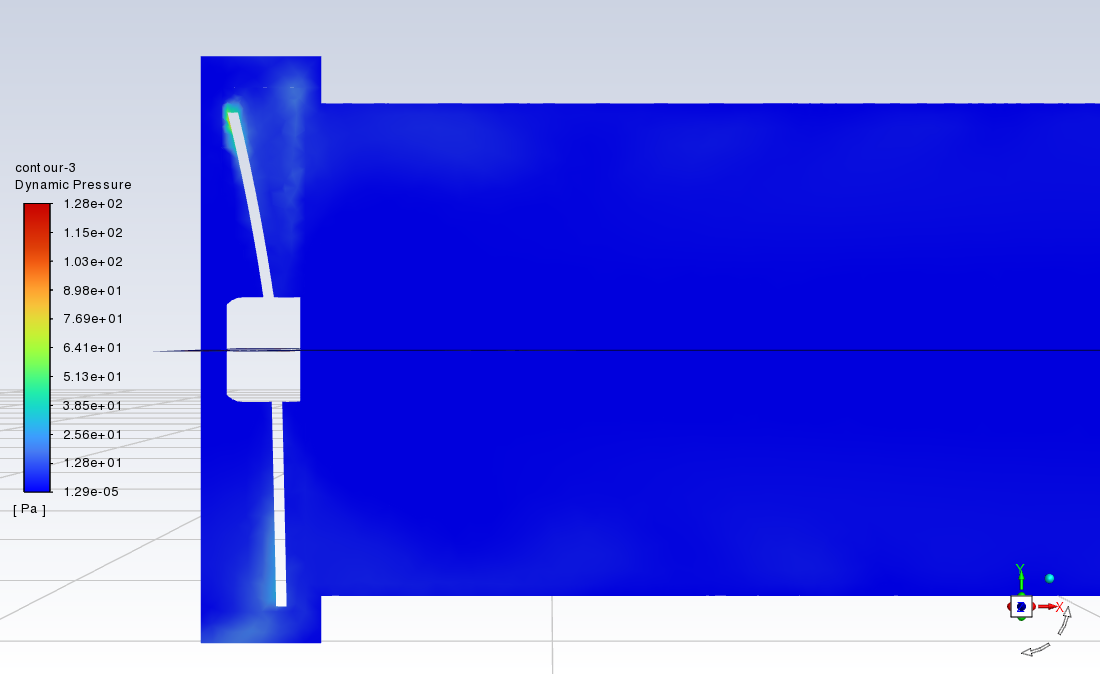
\includegraphics[width=0.6\textwidth]{images/dyn2.png}
    \caption{Mapa de presión dinámica para 2500 RPM.}
    \label{fig:dyn2}
\end{figure}

\begin{figure}[!ht]
    \centering
    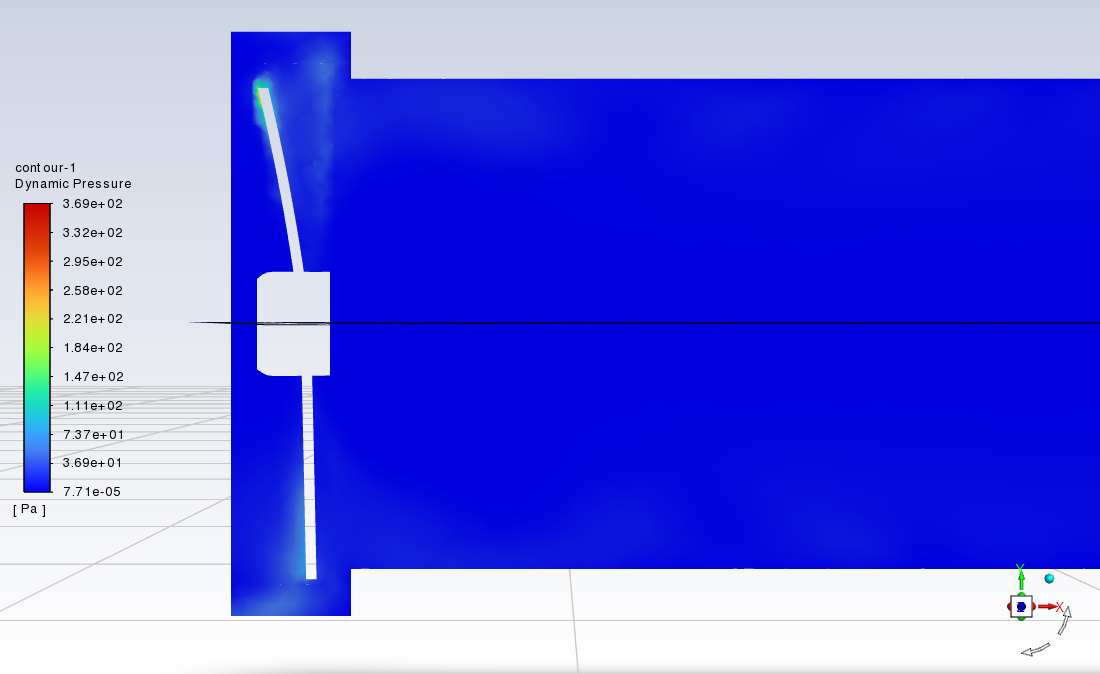
\includegraphics[width=0.6\textwidth]{images/dyn3.png}
    \caption{Mapa de presión dinámica para 4200 RPM.}
    \label{fig:dyn3}
\end{figure}

Es posible observar los mayores gradientes de presión generados en las aspas de la cámara de entrada, lo que ocasiona el flujo de entrada de viento.

%%%%%%%%%%%%%%%%%%%%%%%%%%%%%%%%%%%%%%%%%%%%%%%%%%%%%%%%%%%%%%%%%%%%%
\newpage
\subsection{Lineas de corrientes}

En las figuras \ref{fig:cor1}-\ref{fig:cor3} se presentan las lineas de corriente para los casos simulados, coloreadas según su velocidad.

\begin{figure}[ht!]
    \centering
    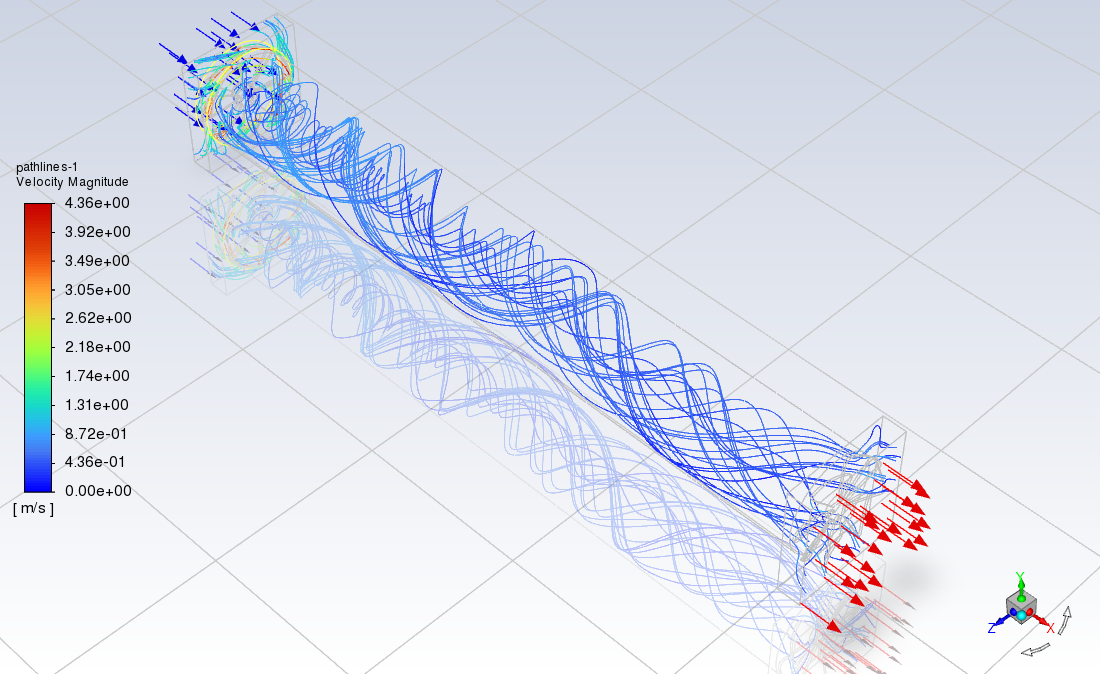
\includegraphics[width=0.9\textwidth]{images/cor1.png}
    \caption{Lineas de corriente para 833 RPM.}
    \label{fig:cor1}
\end{figure}

\begin{figure}[ht!]
    \centering
    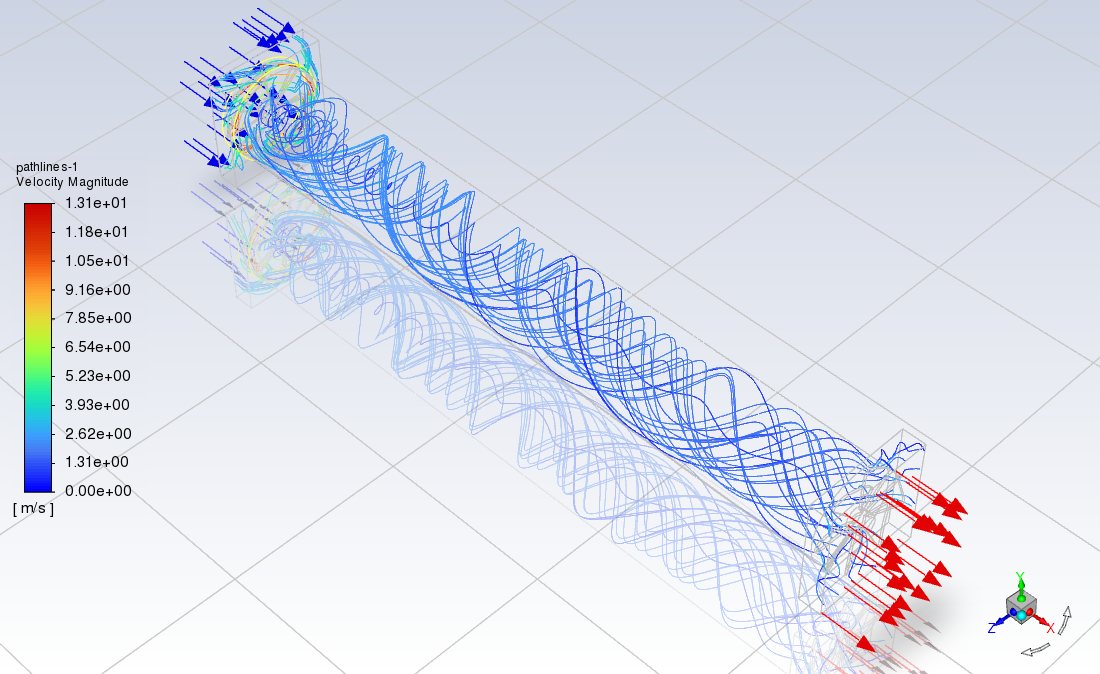
\includegraphics[width=0.9\textwidth]{images/cor2.png}
    \caption{Lineas de corriente para 2500 RPM.}
    \label{fig:cor2}
\end{figure}

\pagebreak
\begin{figure}[ht!]
    \centering
    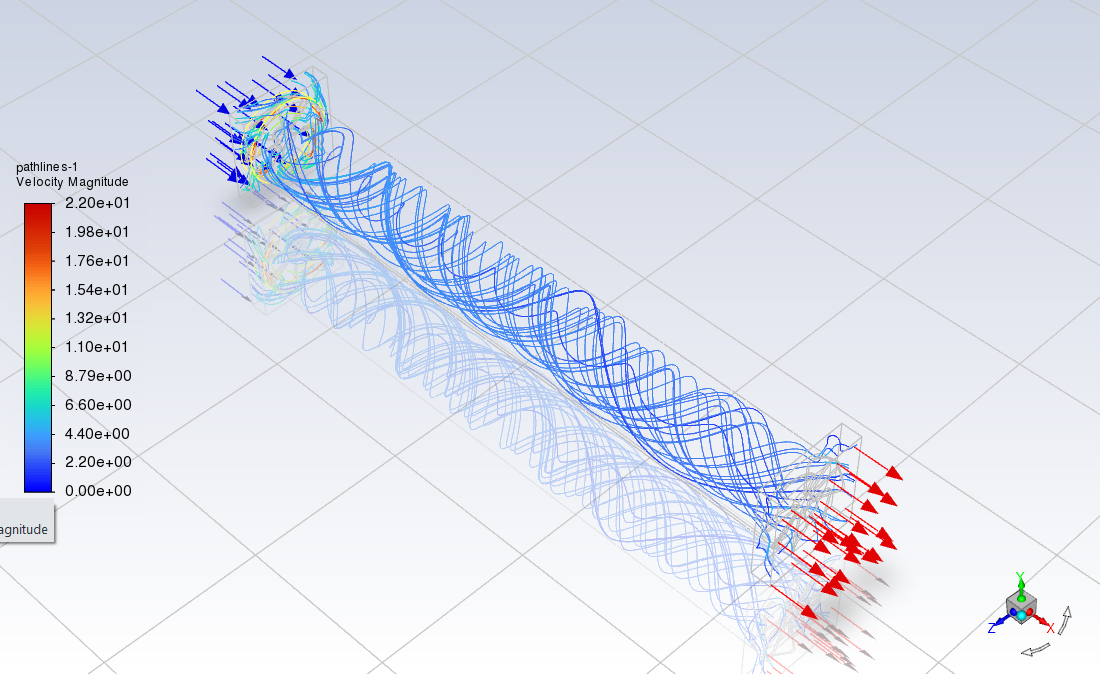
\includegraphics[width=0.9\textwidth]{images/cor3.png}
    \caption{Lineas de corriente para 4200 RPM.}
    \label{fig:cor3}
\end{figure}

Se puede notar como a mayor velocidad de rotación del ventilador incrementa la velocidad y frecuencia de remolinos en la zona perimetral del túnel.

%%%%%%%%%%%%%%%%%%%%%%%%%%%%%%%%%%%%%%%%%%%%%%%%%%%%%%%%%%%%%%%%%%%%%
\subsection{Mapas de velocidad en la cámara de salida}

Se analiza la sección transversal de la cámara de salida para extraer datos de la velocidad de flujo de viento simulado en la salida del túnel de viento para los distintos casos. En base a los datos conseguidos se realizaron promedios integrales sobre el área equivalente del instrumento de medición de velocidad del viento (diámetro de 110mm) para realizar la validación del modelo. Los mapas de velocidad de salida se muestran en las figuras \ref{fig:sal1}-\ref{fig:sal3}.

\begin{figure}[ht!]
    \centering
    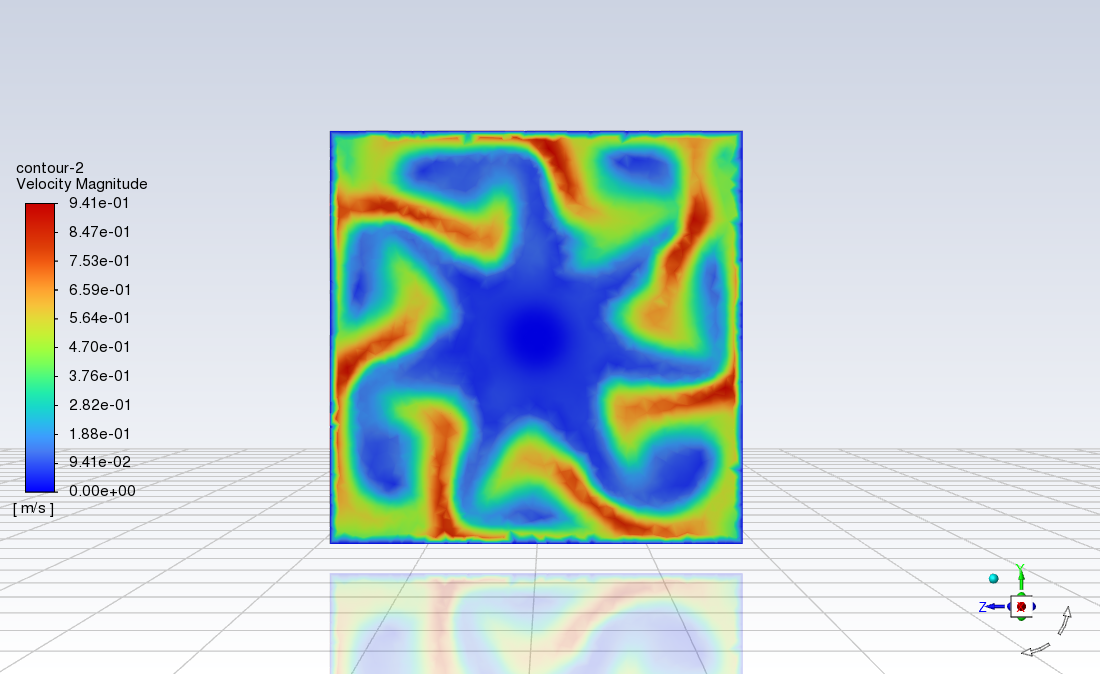
\includegraphics[width=0.6\textwidth]{images/sal1.png}
    \caption{Mapa de velocidad en la salida para 833 RPM.}
    \label{fig:sal1}
\end{figure}

\pagebreak

\begin{figure}[ht!]
    \centering
    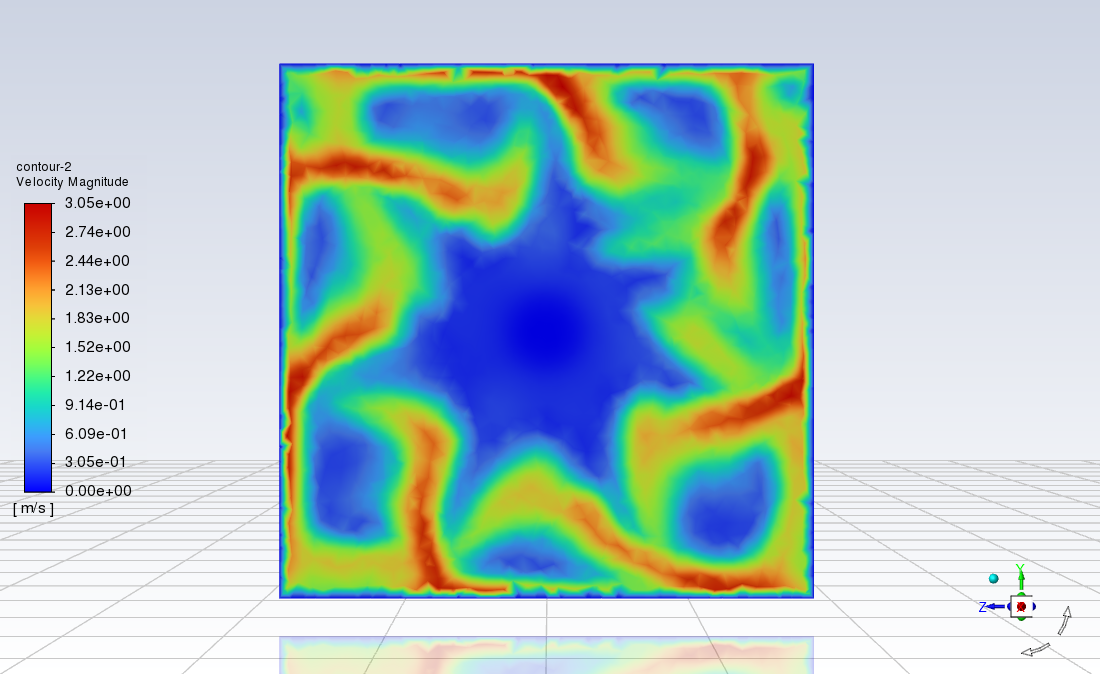
\includegraphics[width=0.6\textwidth]{images/sal2.png}
    \caption{Mapa de velocidad en la salida para 2500 RPM.}
    \label{fig:sal2}
\end{figure}

\begin{figure}[ht!]
    \centering
    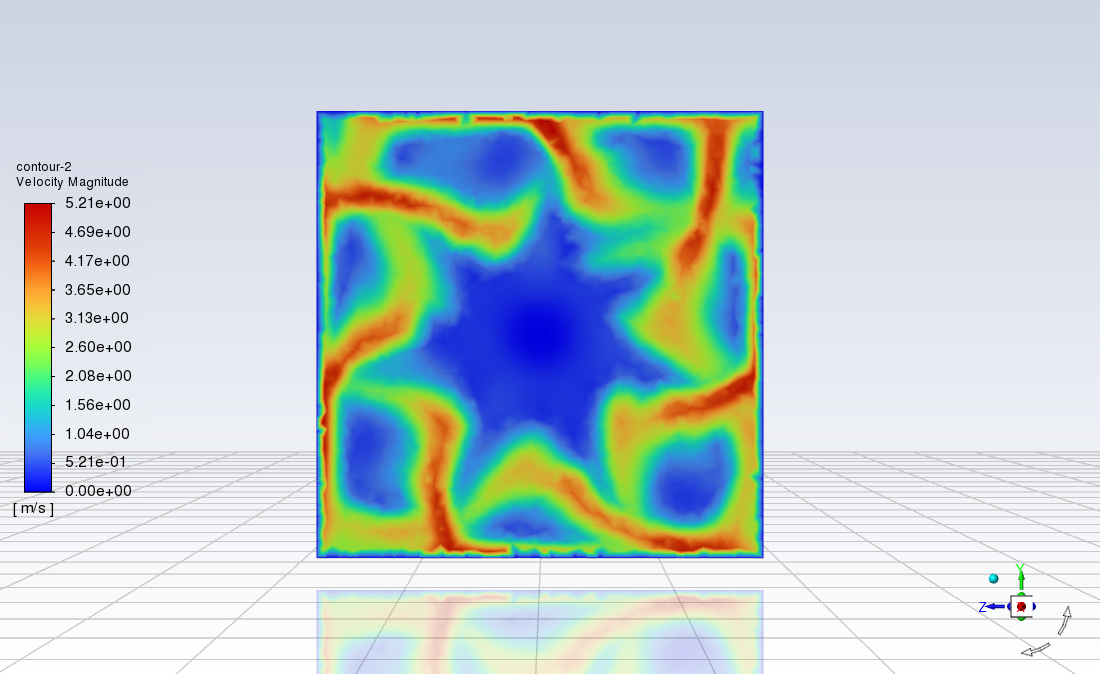
\includegraphics[width=0.6\textwidth]{images/sal3.png}
    \caption{Mapa de velocidad en la salida para 4200 RPM.}
    \label{fig:sal3}
\end{figure}

Se observa como debido a la obstrucción del anemómetro en la cámara de salida se generan zonas de alta velocidad en los alrededores de las aspas. 

%%%%%%%%%%%%%%%%%%%%%%%%%%%%%%%%%%%%%%%%%%%%%%%%%%%%%%%%%%%%%%%%%%%%%
\newpage
\section{Comparación de Velocidad de Flujo de Aire a Distintas RPM}
\subsection{Mediciones Experimentales vs. Simulación}
Para la validación cuantitativa, se midieron las velocidades promedio en la cámara principal a una distancia de aproximadamente 690 mm del ventilador, utilizando el sensor de flujo de aire indirecto y un anemómetro calibrado de 110mm de diámetro. Se utiliza una integral de área sobre la superficie correspondiente al anemómetro para determinar la velocidad. En la Tabla \ref{tab:comp_velocidades} se listan los valores medios experimentales (\(\bar{v}_{\text{exp}}\)) y los simulados (\(\bar{v}_{\text{sim}}\)), junto con el porcentaje de error relativo.

\begin{table}[htbp]
    \centering
    \caption{Comparación de velocidades promedio medidas y simuladas a diferentes RPM del ventilador.}
    \label{tab:comp_velocidades}
    \begin{tabular}{cccccc}
    \toprule
    \multirow{2}{*}{\textbf{RPM}} & \multicolumn{2}{c}{\textbf{Velocidad (m/s)}} & \multirow{2}{*}{\textbf{Error \%}} \\
    \cmidrule(r){2-3}
    & $\bar{v}_{\text{exp}}$ & $\bar{v}_{\text{sim}}$ &  \\
    \midrule
    833 & 0.63 & 0.46 & 26.98\% \\
    2500 & 1.80 & 1.34 & 25.56\% \\
    4200 & 2.75 & 2.12 & 22.91\% \\
    \bottomrule
    \end{tabular}
\end{table}

Se observó que el error porcentual promedio se ubicó cerca de 25\%, valor considerado aceptable para un prototipo a escala, dados los supuestos simplificadores (geometría idealizada y simplificada, supuestas condiciones isotérmicas y ausencia de pérdidas detalladas en el eje del ventilador).

\subsection{Análisis de Resultados}
Los resultados muestran una tendencia coherente: a medida que se incrementa la velocidad de giro del ventilador, el flujo de aire presenta mayor velocidad tanto en el experimento como en la simulación. La presencia de un error prácticamente constante sugiere que el modelo CFD capta de manera consistente la dinámica del flujo, aunque podrían afinarse ciertos aspectos (malla en la zona del impulsor o modelos de turbulencia más avanzados) para disminuir la diferencia.

\section{Resumen de los Resultados}
En conclusión, se logró:
\begin{itemize}
    \item Implementar una \textbf{plataforma de control y adquisición de datos} funcional, basada en Arduino, una REST API y un panel web, con almacenamiento ligero en SQLite.
    \item Obtener \textbf{mediciones experimentales} confiables de corriente, voltaje, temperatura, vibración y velocidad de aire en el túnel de viento a escala.
    \item Desarrollar un \textbf{modelo CFD} en ANSYS cuyos resultados de velocidad de flujo muestran concordancia satisfactoria (errores promedios del orden de 25\%) frente a los datos reales en un rango de 833 a 4200 RPM.
\end{itemize}

Estos hallazgos sientan las bases para la validación del sistema y aportan indicios de que las metodologías propuestas —tanto la plataforma de medición como el modelo de simulación— pueden escalarse a condiciones mineras reales o utilizarse como punto de partida para implementar algoritmos de mantenimiento predictivo.

%%%%%%%%%%%%%%%%%%%%%%%%%%%%%%%%%%%%%%%%%%%%%%%%%%%%%%%%%%%%%%%%%%%%
\section{Evaluación Cualitativa de Datos}

Tras aplicar la metodología descrita para la evaluación cualitativa de los datos, se obtuvieron los siguientes hallazgos principales:

\subsection{Patrones de Operación Observados}
\begin{itemize}
    \item \textbf{Rangos de RPM estables:} En la mayoría de los ensayos, se identificó un rango de revoluciones (aproximadamente entre 833 y 4200 RPM) en el cual el ventilador mantiene un comportamiento estable, con lecturas de corriente y vibraciones relativamente constantes.
    \item \textbf{Regiones de posible sobrefuerzo:} No fue posible detectar zonas de sobreesfuerzo. El comportamiento fue nominal para todas las velocidades sin mayores variaciones en temperatura.
\end{itemize}

\subsection{Comparación Cualitativa entre Datos Experimentales y Simulación}
\begin{itemize}
    \item \textbf{Similitud en la distribución de velocidades:} Las mediciones reales de la velocidad del viento (mediante el anemómetro) mostraron valores de magnitud coherentes con los obtenidos en la simulación CFD, especialmente en el rango medio de velocidades.
    \item \textbf{Impacto de vibraciones y pérdidas:} El prototipo experimental presentó vibraciones adicionales que no se capturaron en la simulación, lo que sugiere que, para mejorar la concordancia, habría que refinar el modelado mecánico y acoplarlo a los fenómenos fluidodinámicos.
\end{itemize}

\subsection{Relaciones entre Variables Clave}
\begin{itemize}
    \item \textbf{RPM--Vibraciones:} Se constató que, en general, un incremento progresivo de RPM se asocia con mayores valores de vibración.
    \item \textbf{RPM--Velocidad del Viento:} Existió una correlación directa y estable en la mayor parte de los ensayos.
    \item \textbf{Corriente--Temperatura:} Al aumentar la carga eléctrica, no fue posible registrar grandes cambios de temperatura, lo que sugiere que el ventilador opera en su rango nominal y no se está sobreesforzando.
\end{itemize}

\subsection{Posible Viabilidad de un Modelo Predictivo}
\begin{itemize}
    \item \textbf{Variedad de datos:} La existencia de mediciones tanto en condiciones normales como en regímenes de sobreesfuerzo sugiere que los conjuntos de datos cuentan con cierto grado de diversidad. Esto resulta prometedor para futuros enfoques predictivos.
    \item \textbf{Inconsistencias menores:} Aunque se detectaron disparidades en escenarios de alta RPM, la mayor parte de la información muestra coherencia interna suficiente como para servir de base a un análisis más profundo y a la eventual creación de un modelo de mantenimiento predictivo.
    \item \textbf{Posibles Variables Complementarias:} La incorporación de más señales (por ejemplo, análisis de espectros de vibración o monitoreo del desgaste físico en el tiempo) podría incrementar la confianza y robustez de un futuro modelo.
\end{itemize}

\noindent
En términos generales, la evaluación cualitativa muestra que los datos disponibles describen de forma razonable el comportamiento del ventilador a diferentes regímenes de operación. Existe una relación consistente entre las variables clave (RPM, velocidad de viento, vibraciones), lo cual se considera indicio de que sería factible avanzar hacia modelos más sofisticados de predicción y mantenimiento si se profundiza

\chapter{Discusión}

En este capítulo se analizan críticamente los resultados presentados en el capítulo anterior, evaluando el desempeño del modelo de túnel de viento a escala y la eficacia de la plataforma de adquisición de datos y de la simulación CFD en ANSYS. Además, se exponen las limitaciones encontradas, así como las oportunidades de mejora y de futuras extensiones al proyecto.

\section{Evaluación de la Plataforma de Control y Adquisición de Datos}
La plataforma desarrollada, basada en un microcontrolador Arduino, un servicio REST API y una interfaz web, demostró la capacidad de configurar y monitorizar en tiempo real los parámetros clave del túnel de viento a escala. El almacenamiento en la base de datos SQLite permitió gestionar y consultar los datos de forma ágil, facilitando la explotación analítica posterior.

\subsection{Contribuciones Relevantes}
\begin{itemize}
    \item \textbf{Flexibilidad operativa:} La interfaz web ofreció un control manual o automático de la velocidad del ventilador, lo que habilitó la realización de distintos tipos de pruebas experimentales sin requerir modificaciones de hardware.
    \item \textbf{Ahorro de tiempo y accesibilidad:} Al permitir ajustes rápidos de configuración y la visualización de los datos en tiempo real, se redujo la necesidad de reconfigurar o detener completamente el sistema para la toma de mediciones.
    \item \textbf{Escalabilidad:} A pesar de haber sido diseñada para un prototipo a escala, la arquitectura modular de la plataforma puede migrarse a sistemas con más sensores y mayor volumen de datos, conservando la misma lógica de API y almacenamiento.
\end{itemize}

\subsection{Limitaciones}
\begin{itemize}
    \item \textbf{Rendimiento en entornos con muchos sensores:} Durante los ensayos se empleó un número limitado de sensores. La integración de más dispositivos podría requerir optimizaciones en la transmisión de datos, tasas de muestreo o incluso en el tipo de base de datos.
    \item \textbf{Dependencia de la conexión:} Si bien se probaron conexión serial y Wi-Fi, en escenarios mineros reales la estabilidad de la comunicación es crucial, por lo que deberían considerarse protocolos industriales robustos o redundancia en la red.
\end{itemize}

\section{Análisis de las Mediciones Experimentales}
\subsection{Exactitud y Robustez de los Sensores}
Los resultados mostraron coherencia interna en las mediciones de corriente, voltaje, flujo de aire, temperatura y vibración. Se comprobó que los sensores, cuando se calibran correctamente, ofrecen un nivel de precisión adecuado para un prototipo de baja escala. No obstante, algunas imprecisiones pueden originarse en:
\begin{itemize}
    \item \textbf{Deriva térmica y electrónica:} Sensores como el LM35 y el anemómetro pueden presentar desviaciones tras periodos prolongados de operación.
    \item \textbf{Ruido en señales analógicas:} Aunque se emplearon condensadores de filtrado, la cercanía física de varios sensores y la alimentación compartida pueden introducir pequeñas fluctuaciones.
\end{itemize}

\subsection{Variabilidad en la Velocidad de Flujo}
Algunas oscilaciones en la velocidad de flujo medidas por el anemómetro podrían deberse a:
\begin{itemize}
    \item \textbf{Turbulencias locales:} Pequeñas turbulencias o recirculaciones cercanas a las paredes del túnel.
    \item \textbf{Cambios en la velocidad del ventilador:} La señal PWM no siempre es perfectamente estable, especialmente a frecuencias bajas.
\end{itemize}

A pesar de esto, la repetitividad de los resultados sugiere que el sistema de medición cuenta con un margen de error aceptable para la validación comparativa con la simulación CFD.

\section{Discusión de la Simulación CFD}
\subsection{Selección del Modelo y Parámetros Numéricos}
La elección del modelo de turbulencia \texttt{k-$\epsilon$} estándar y las simplificaciones geométricas (por ejemplo, la idealización de las aspas del ventilador) tuvieron un impacto en la exactitud de la simulación. La constatación de un error porcentual del orden de 7\,\% en la velocidad de flujo sugiere que, si se buscase mayor precisión, podrían considerarse:
\begin{itemize}
    \item Modelos de turbulencia más avanzados (\texttt{k-$\omega$}, SST o incluso RSM) para capturar las fluctuaciones del flujo y las zonas de recirculación con mayor fidelidad.
    \item Una malla refinada en la proximidad del rotor, aplicando modelos de capa límite que mejoren el cálculo de las velocidades cercanas a las paredes del ventilador y del túnel.
    \item Simulaciones transitorias (no estacionarias), que podrían reflejar mejor la naturaleza pulsante del flujo, especialmente a RPM más altas.
\end{itemize}

\subsection{Comparación con Datos Experimentales}
La correlación entre los valores de velocidad simulados y medidos fue consistentemente aceptable en los tres puntos de operación estudiados (833, 2500 y 4200 RPM). Esto indica que, en términos globales, el modelo numérico predice correctamente la tendencia de incremento del flujo de aire con el aumento de las RPM, lo que valida tanto la aproximación del método como la fiabilidad de las mediciones.

\section{Síntesis de la Comparación Experimental-Simulación}
\begin{itemize}
    \item \textbf{Coincidencia de tendencias:} Tanto los datos experimentales como los resultados de CFD muestran que el flujo de aire se incrementa proporcionalmente con la velocidad del ventilador, confirmando el comportamiento esperado.
    \item \textbf{Discrepancias razonables:} Las diferencias se mantuvieron por debajo del 10\,\%, lo cual se considera aceptable para un estudio a escala. Parte de estas discrepancias podrían atribuirse a condiciones de contorno ideales en la simulación frente a condiciones reales en el prototipo (pérdidas de calor, variaciones de presión ambiente, alineación del ventilador, etc.).
\end{itemize}

\section{Implicaciones para el Mantenimiento Predictivo}
Aunque la validación se enfocó en el flujo de aire, el sistema de adquisición integra también sensores de corriente, voltaje y vibración, variables de gran relevancia para el mantenimiento predictivo. El hecho de que estas mediciones se realicen de manera continua abre la posibilidad de:
\begin{itemize}
    \item Identificar patrones de desgaste o desequilibrio del ventilador a lo largo del tiempo.
    \item Correlacionar el incremento de consumo de potencia eléctrica con posibles obstrucciones o deterioro en las aspas del ventilador.
    \item Adoptar estrategias de mantenimiento condicional basadas en umbrales (por ejemplo, vibración excesiva o calentamiento anormal) para anticiparse a fallas.
\end{itemize}
Estos aspectos no formaron parte principal de la discusión en este estudio, pero el sistema desarrollado sienta las bases para su implementación futura.

\section{Limitaciones del Estudio}
\begin{itemize}
    \item \textbf{Escalabilidad a entornos reales:} El prototipo se diseñó a una escala reducida, por lo que, si bien la metodología es extrapolable, las condiciones de presión y temperatura en una mina real podrían requerir modelos más complejos y soluciones de ingeniería a mayor escala.
    \item \textbf{Restricción de variables analizadas:} El foco principal fue la validación del flujo de aire y la comparación con la potencia consumida y la vibración. El proyecto no abarcó la simulación detallada de la transferencia de calor o la influencia de contaminantes en el flujo.
    \item \textbf{Modelo simplificado del ventilador:} Se empleó una aproximación genérica para simular la zona de rotación del ventilador. Un modelado más detallado del impulsor y de las palas podría refinar la precisión de las predicciones de velocidad.
\end{itemize}

\section{Oportunidades de Mejora y Trabajo Futuro}
Con base en los resultados y las observaciones anteriores, se vislumbran varias líneas de desarrollo:
\begin{itemize}
    \item \textbf{Mejora de la simulación CFD:} Implementar modelos de turbulencia más sofisticados o simulaciones transitorias para afinar la predicción de zonas de recirculación y fluctuaciones de flujo.
    \item \textbf{Ampliación de la instrumentación:} Añadir sensores de presión diferencial a lo largo del túnel para una validación más exhaustiva del campo de presiones.
    \item \textbf{Incorporación de Machine Learning:} Aprovechar las mediciones continuas para entrenar modelos de aprendizaje automático que anticipen cambios en la eficiencia del ventilador o inicios de fallas mecánicas.
    \item \textbf{Escenarios más cercanos a minería real:} Experimentar con variaciones de temperatura o humedad que aproximen las condiciones subterráneas, y evaluar el impacto de la presencia de polvo o partículas en el flujo de aire.
\end{itemize}

\section{Conclusiones de la Discusión}
La construcción de un túnel de viento a escala y su integración con un sistema automatizado de adquisición de datos y un modelo CFD han demostrado ser efectivos para analizar y validar el comportamiento de un ventilador sometido a diferentes velocidades. A pesar de las simplificaciones inherentes al prototipo y a la simulación, el acuerdo entre los datos experimentales y numéricos fue satisfactorio. 

Desde un punto de vista metodológico, este trabajo aporta un marco reproducible para la experimentación y validación de modelos CFD, con posibilidades de expansión hacia estrategias de mantenimiento predictivo. Los hallazgos, finalmente, subrayan la necesidad de una aproximación combinada (experimentación + modelado + análisis de datos) para afrontar los desafíos de la ventilación y el control de equipos rotativos en entornos mineros.

\chapter{Conclusiones y Recomendaciones}

En este capítulo se presenta un resumen de los principales hallazgos y aportes del estudio, se describen las implicaciones en torno al mantenimiento predictivo y se plantean posibles líneas de investigación futuras para profundizar y ampliar los resultados obtenidos.

\section{Conclusiones del Estudio}
\begin{enumerate}
    \item \textbf{Diseño y construcción del túnel de viento a escala:}  
    La implementación de un prototipo con estructura modular permitió reproducir de forma simplificada las condiciones de ventilación minera. Se validó la robustez mecánica del sistema y se logró un montaje estable del ventilador y de los sensores, asegurando mediciones representativas de variables como corriente, voltaje, flujo de aire, temperatura y vibración.

    \item \textbf{Plataforma de adquisición de datos y control:}  
    El uso de Arduino para la lectura de sensores, junto con un servicio REST API y una interfaz web, demostró ser una solución ágil y escalable. La base de datos SQLite manejó de forma satisfactoria el almacenamiento y la consulta de información, facilitando la generación de históricos y la exportación de los resultados para su análisis.

    \item \textbf{Simulación CFD en ANSYS:}  
    El modelo numérico desarrollado para analizar la dinámica del flujo de aire dentro del túnel mostró un error promedio de aproximadamente 25\,\% al comparar las velocidades simuladas con las medidas, lo que se consideró aceptable dada la escala del prototipo y los supuestos simplificadores (condiciones de contorno ideales, modelo de turbulencia genérico, entre otros). Los campos de velocidad y las zonas de recirculación obtenidas en la simulación fueron coherentes con la evidencia experimental.

    \item \textbf{Validación de la metodología:}  
    La correlación entre los datos experimentales y la simulación CFD confirmó la eficacia de la metodología propuesta para caracterizar y estimar el comportamiento aerodinámico del sistema. Este marco de trabajo puede escalarse a ventiladores de mayor tamaño o incorporarse a un entorno minero real, con los ajustes pertinentes en la geometría del túnel y en las condiciones de operación.

    \item \textbf{Visión integral de la instrumentación y la simulación:}  
    El enfoque combinado —instrumentación real y modelado computacional— brindó una plataforma sólida para entender y optimizar el funcionamiento del ventilador. A su vez, sentó las bases para la integración de técnicas de mantenimiento predictivo.

\end{enumerate}

\section{Implicaciones para el Mantenimiento Predictivo}
\begin{enumerate}
    \item \textbf{Monitoreo continuo de variables clave:}  
    La plataforma desarrollada permite registrar parámetros como corriente, voltaje y vibración de manera continua. Estos indicadores se asocian a fallas incipientes en equipos rotativos; por tanto, su monitoreo posibilita diagnosticar problemas mecánicos o eléctricos antes de que se tornen críticos.

    \item \textbf{Correlación con modelos CFD:}  
    Al comparar los valores reales de flujo de aire con los resultados simulados, se puede trazar un perfil “ideal” o de referencia para el ventilador. Cualquier desviación relevante en las velocidades medidas podría indicar pérdidas de eficiencia o daños estructurales, lo cual permitiría programar intervenciones de mantenimiento de forma temprana.

    \item \textbf{Base de datos para aprendizaje automático:}  
    El sistema de adquisición y almacenamiento en SQLite genera un histórico de datos continuo. Dicho histórico constituye la materia prima para entrenar algoritmos de machine learning o análisis predictivo, capaces de detectar patrones que anticipen la aparición de fallas o el desgaste de componentes.

    \item \textbf{Reducción de costos y tiempos de inactividad:}  
    La adopción de estrategias de mantenimiento basadas en condición, sustentadas en la información proveniente de la plataforma, reduce la probabilidad de fallas inesperadas. Esto significa menores tiempos de inactividad y optimización de los recursos empleados en reparaciones, con impacto económico positivo.
\end{enumerate}

\section{Recomendaciones para Futuras Investigaciones}
\begin{enumerate}
    \item \textbf{Refinamiento del modelo CFD:}  
    Para obtener mayor precisión en la predicción de velocidad y en la caracterización del flujo, podrían aplicarse modelos de turbulencia más avanzados (\texttt{k-$\omega$} SST o RSM) o simulaciones transitorias (DES o LES). También se recomienda refinar la malla en regiones críticas, como la zona del impulsor.

    \item \textbf{Expansión de la instrumentación:}  
    Incluir sensores de presión diferencial y sensores de gases ayudaría a representar mejor las condiciones reales de la minería subterránea, donde la ventilación cumple el rol fundamental de disipar contaminantes y controlar la temperatura.

    \item \textbf{Incorporación de técnicas de aprendizaje automático:}  
    El histórico de datos recogidos puede emplearse para entrenar modelos que predigan la evolución de variables como la vibración o el consumo energético, facilitando la detección temprana de anomalías. Se sugiere explorar algoritmos de clasificación y regresión con redes neuronales o métodos de árboles de decisión.

    \item \textbf{Pruebas a mayor escala y en entornos más cercanos a la minería real:}  
    Para validar la viabilidad de la propuesta en un entorno industrial, se recomienda la construcción de un prototipo de dimensiones mayores o la adaptación del sistema a un ventilador minero existente, teniendo en cuenta parámetros como presión, polvo, humedad y temperatura extrema.

    \item \textbf{Análisis de la rentabilidad y ROI de la implementación:}  
    Se podrían realizar estudios económicos que comparen el costo de inversión en instrumentación y software de simulación con los ahorros derivados de un mantenimiento predictivo más eficaz, de forma que se cuantifique el impacto financiero de la adopción de estas tecnologías.
\end{enumerate}

En suma, los resultados de esta investigación confirman la viabilidad y utilidad de la metodología propuesta para estudiar, evaluar y optimizar el funcionamiento de un sistema de ventilación, sentando a la vez las bases para estrategias de mantenimiento predictivo. La coherencia de los datos experimentales y los modelos CFD refuerza la confiabilidad de la aproximación, abriendo camino a nuevas investigaciones y desarrollos que podrían acercar este prototipo experimental a aplicaciones reales en la industria minera.


%%%%%%%%%%%%%%%%%%%%%%%%%%%%%%%%%%%%%%%%%%%%%%%%%%%%%%%%%%%%%%%%%%%%%%%%%%%%%%%%%%%%%%%%%%%%%%%%%%%%%%%%%

%%%%%  BIBLIOGRAFÍA %%%

\singlespacing
\backmatter
\phantomsection  % para ajustar el hyperref
\def\thispagestyle#1{}
\addcontentsline{toc}{chapter}{Bibliografía}
\addtocontents{bibliography}{\protect\thispagestyle{fancy}} %forzar fancy en table of contents Lof.
\addtocontents{bibliography} %forzar fancy en table of contents Lof.
\makeatother
\makeatletter

\printbibliography

%%% APÉNDICES Y ANEXOS  %%%%%%%%%%%
\mainmatter %%% empieza la numeración para los apéndices
\appendix   %%% preámbulo para que aparezcan apéndices
\clearpage
\noappendicestocpagenum
\addappheadtotoc   %%los apéndices se separan del resto en el indice
\appendixpage

%\chapter{Apéndices}
\thispagestyle{fancy}
\section{Informe Técnico de ..}
%\lipsum[1-4].
\section{Plan de..}
%\lipsum[1-4].
 % APÉNDICES
\chapter{Anexos}
\thispagestyle{fancy}

\appendix
\renewcommand\thesection{\Alph{section}}
\section{Códigos y Scripts de Modelo Experimental}
En esta sección se incluyen fragmentos de los códigos empleados para la adquisición de datos para una placa ESP32 TTGO T-Display.

\subsection{Script de Configuración del Arduino}

\begin{verbatim}
    #include <WiFi.h>
    #include <WebServer.h>
    #include <TFT_eSPI.h>
    #include <Wire.h>
    #include <Adafruit_AMG88xx.h>
    #include <Adafruit_ADXL345_U.h>    // Replaced MPU6050 library with ADXL345
    #include <Adafruit_Sensor.h>
    #include "xbm.h"                   // Sketch tab header for xbm images
    #include <ArduinoJson.h>           // Include ArduinoJson library
    
    // ===================== PIN DEFINITIONS =====================
    
    // LM35 sensor pin
    #define LM35_PIN       33 // GPIO33 (ADC1_CH5)
    
    // Voltage input pin (if still needed for a generic voltage measurement)
    #define VOLTAGE_PIN    32 // GPIO32 (ADC1_CH4)
    
    // FZ0430 voltage sensor pin (adjust as needed)
    #define FZ0430_PIN     34 // Example: GPIO34 (ADC1_CH6)
    
    // ACS712 current sensor pin (adjust as needed)
    #define ACS712_PIN     36 // Example: GPIO36
    
    // PWM output pin (fan control, etc.)
    #define PWM_PIN        25 // GPIO25
    
    // I2C pins (ESP32 default)
    #define SDA_PIN        21
    #define SCL_PIN        22
    
    // Button pins
    #define BUTTON_LEFT_PIN  0   // GPIO0  - Left Button
    #define BUTTON_RIGHT_PIN 35  // GPIO35 - Right Button
    
    // ===================== OBJECTS & GLOBALS =====================
    TFT_eSPI tft = TFT_eSPI();
    WebServer server(80);
    
    Adafruit_AMG88xx amg;       
    Adafruit_ADXL345_Unified adxl = Adafruit_ADXL345_Unified(12345);
    
    int pwmValue = 0;  // PWM value for fan control
    
    const char* ssid = "Network";      // Replace with your Wi-Fi SSID
    const char* password = "Password"; // Replace with your Wi-Fi password
    
    // Cache for ADXL345 at 100Hz
    sensors_event_t cachedAccelEvent;
    unsigned long lastMPUReadTime = 0;
    const unsigned long mpuReadInterval = 10; // Read every 10 ms (100 Hz)
    
    // Update display
    unsigned long lastDisplayUpdateTime = 0;
    const unsigned long displayUpdateInterval = 500;
    
    // Button read timing
    unsigned long lastButtonReadTime = 0;
    const unsigned long buttonReadInterval = 250;
    
    String ipAddress;
    
    // PWM control variables
    int pwmLevel = 0;             
    const int maxPwmLevel = 10;   
    
    // Button press timing variables
    unsigned long buttonLeftPressedTime = 0;
    unsigned long buttonRightPressedTime = 0;
    const unsigned long longPressDuration = 1000; // 1 second for long press
    
    // Last button states
    bool buttonLeftLastState = HIGH;
    bool buttonRightLastState = HIGH;
    
    // ===================== CORS HELPER =====================
    void sendCORSHeaders() {
      server.sendHeader("Access-Control-Allow-Origin", "*");
      server.sendHeader("Access-Control-Allow-Methods", "GET, POST, OPTIONS");
      server.sendHeader("Access-Control-Allow-Headers", "Content-Type");
    }
    
    // ===================== HANDLERS =====================
    
    // Handle LM35 - returns {"value": <number>}
    void handleLM35() {
      int analogValue = analogRead(LM35_PIN);
      float voltage = analogValue * (3.3 / 4095.0);
      float temperatureC = voltage * 100.0;
    
      StaticJsonDocument<200> jsonResponse;
      jsonResponse["value"] = temperatureC;
    
      String response;
      serializeJson(jsonResponse, response);
    
      sendCORSHeaders();
      server.send(200, "application/json", response);
    }
    
    // Handle Voltage (generic) - returns {"value": <number>}
    void handleVoltage() {
      int analogValue = analogRead(VOLTAGE_PIN);
      float voltage = analogValue * (3.3 / 4095.0);
      float inputVoltage = voltage * (5.0 / 3.3);
    
      StaticJsonDocument<200> jsonResponse;
      jsonResponse["value"] = inputVoltage;
    
      String response;
      serializeJson(jsonResponse, response);
    
      sendCORSHeaders();
      server.send(200, "application/json", response);
    }
    
    // Handle ADXL345 - returns {"x": <number>, "y": <number>, "z": <number>}
    void handleADXL345() {
      StaticJsonDocument<200> jsonResponse;
      jsonResponse["x"] = cachedAccelEvent.acceleration.x;
      jsonResponse["y"] = cachedAccelEvent.acceleration.y;
      jsonResponse["z"] = cachedAccelEvent.acceleration.z;
    
      String response;
      serializeJson(jsonResponse, response);
    
      sendCORSHeaders();
      server.send(200, "application/json", response);
    }
    
    // Handle AMG8833 - returns {"grid": [[8 values], [8 values], ...]}
    void handleAMG8833() {
      float pixels[64];
      amg.readPixels(pixels);
    
      StaticJsonDocument<2048> jsonResponse; // Larger document for 8x8 data
      JsonArray grid = jsonResponse.createNestedArray("grid");
    
      for (int row = 0; row < 8; row++) {
        JsonArray rowArray = grid.createNestedArray();
        for (int col = 0; col < 8; col++) {
          rowArray.add(pixels[row * 8 + col]);
        }
      }
    
      String response;
      serializeJson(jsonResponse, response);
    
      sendCORSHeaders();
      server.send(200, "application/json", response);
    }
    
    // Handle setPWM - sets PWM (0-255)
    void handleSetPWM() {
      if (server.hasArg("value")) {
        sendCORSHeaders();
        String valueStr = server.arg("value");
        int value = valueStr.toInt();
        if (value >= 0 && value <= 255) {
          pwmValue = value;
          analogWrite(PWM_PIN, pwmValue);
          server.send(200, "text/plain", "PWM value set to " + String(pwmValue));
        } else {
          server.send(400, "text/plain", "Invalid PWM value. Must be between 
          0 and 255.");
        }
      } else {
        server.send(400, "text/plain", "PWM value not provided.");
      }
    }
    
    // ===================== NEW SENSOR HANDLERS =====================
    
    /**
     * Handle FZ0430 Voltage Sensor
     * Returns {"value": <voltage>}
     * 
     * Adjust the multiplication factor based on your actual FZ0430 ratio.
     */
    void handleFZ0430() {
      int rawValue = analogRead(FZ0430_PIN);
      // Convert raw ADC reading to voltage (3.3V range, 12-bit ADC => max 4095)
      float measuredVoltage = rawValue * (3.3f / 4095.0f);
    
      // FZ0430 modules often step down higher voltages to ~3.3V range.
      // Adjust the scaling factor to match your sensor's specs.
      // For example, if the sensor divides input voltage by 5:
      float actualVoltage = measuredVoltage * 5.0f;
    
      StaticJsonDocument<200> doc;
      doc["value"] = actualVoltage;
    
      String response;
      serializeJson(doc, response);
    
      sendCORSHeaders();
      server.send(200, "application/json", response);
    }
    
    /**
     * Handle ACS712 Current Sensor
     * Returns {"value": <current>}
     * 
     * Adjust offset and sensitivity based on your ACS712 variant:
     *  - ACS712 5A  => 185 mV/A
     *  - ACS712 20A => 100 mV/A
     *  - ACS712 30A => 66 mV/A
     */
    void handleACS712() {
      int rawValue = analogRead(ACS712_PIN);
      // Convert raw ADC reading to voltage
      float sensorVoltage = rawValue * (3.3f / 4095.0f);
    
      // ACS712 outputs Vcc/2 at 0 A. For 3.3V supply, that's ~1.65 V offset.
      float offset = 3.3f / 2.0f;  
      // Sensitivity in V/A (adjust as appropriate)
      float sensitivity = 0.185f; // for a 5A version
    
      float current = (sensorVoltage - offset) / sensitivity;
    
      StaticJsonDocument<200> doc;
      doc["value"] = current;
    
      String response;
      serializeJson(doc, response);
    
      sendCORSHeaders();
      server.send(200, "application/json", response);
    }
    
    // ===================== SETUP =====================
    void setup() {
      Serial.begin(115200);
    
      tft.init();
      tft.setRotation(0);
      tft.fillScreen(TFT_BLACK);
      tft.setTextColor(TFT_WHITE, TFT_BLACK);
      tft.setTextSize(1);
      tft.setTextWrap(true);
    
      Wire.begin(SDA_PIN, SCL_PIN);
      Wire.setClock(100000);
    
      tft.drawXBitmap(0, 240 - logoHeight - 25, logo, logoWidth,
      logoHeight, TFT_BLUE);
    
      pinMode(LM35_PIN, INPUT);
      pinMode(VOLTAGE_PIN, INPUT);
      pinMode(FZ0430_PIN, INPUT);
      pinMode(ACS712_PIN, INPUT);
      pinMode(PWM_PIN, OUTPUT);
    
      // Initialize AMG8833
      if (!amg.begin()) {
        Serial.println("Failed to initialize AMG8833!");
        tft.println("AMG8833 init failed!");
      } else {
        Serial.println("AMG8833 initialized.");
      }
    
      // Initialize ADXL345
      if (!adxl.begin()) {
        Serial.println("Failed to initialize ADXL345!");
        tft.println("ADXL345 init failed!");
      } else {
        Serial.println("ADXL345 initialized.");
      }
    
      pinMode(BUTTON_LEFT_PIN, INPUT_PULLUP);
      pinMode(BUTTON_RIGHT_PIN, INPUT_PULLUP);
    
      // Wi-Fi connection
      WiFi.begin(ssid, password);
      tft.println("Connecting to WiFi...");
      while (WiFi.status() != WL_CONNECTED) {
        delay(2000);
        Serial.print(".");
      }
      tft.println("WiFi connected!");
      ipAddress = WiFi.localIP().toString();
      tft.println(ipAddress);
      Serial.println(ipAddress);
    
      // ===================== ENDPOINTS =====================
      server.on("/lm35", handleLM35);
      server.on("/amg8833", handleAMG8833);
      server.on("/adxl345", handleADXL345);
      server.on("/voltage", handleVoltage);
      server.on("/setPWM", handleSetPWM);
    
      // New sensor endpoints
      server.on("/fz0430", handleFZ0430);
      server.on("/acs712", handleACS712);
    
      // OPTIONS handlers for CORS preflight if needed
      server.on("/lm35", HTTP_OPTIONS, []() {
        sendCORSHeaders();
        server.send(204);
      });
      server.on("/amg8833", HTTP_OPTIONS, []() {
        sendCORSHeaders();
        server.send(204);
      });
      server.on("/adxl345", HTTP_OPTIONS, []() {
        sendCORSHeaders();
        server.send(204);
      });
      server.on("/voltage", HTTP_OPTIONS, []() {
        sendCORSHeaders();
        server.send(204);
      });
      server.on("/setPWM", HTTP_OPTIONS, []() {
        sendCORSHeaders();
        server.send(204);
      });
      server.on("/fz0430", HTTP_OPTIONS, []() {
        sendCORSHeaders();
        server.send(204);
      });
      server.on("/acs712", HTTP_OPTIONS, []() {
        sendCORSHeaders();
        server.send(204);
      });
    
      server.begin();
      Serial.println("HTTP server started");
    }
    
    // ===================== LOOP =====================
    void loop() {
      server.handleClient();
    
      unsigned long currentTime = millis();
    
      // ========== Handle Buttons ==========
      if (currentTime - lastButtonReadTime >= buttonReadInterval) {
        lastButtonReadTime = currentTime;
    
        bool buttonLeftState = digitalRead(BUTTON_LEFT_PIN);
        bool buttonRightState = digitalRead(BUTTON_RIGHT_PIN);
    
        // Handle Left Button
        if (buttonLeftLastState == HIGH && buttonLeftState == LOW) {
          buttonLeftPressedTime = currentTime;
        } else if (buttonLeftLastState == LOW && buttonLeftState == HIGH) {
          if (currentTime - buttonLeftPressedTime >= longPressDuration) {
            // Long press => reset PWM to 0
            pwmLevel = 0;
          } else {
            // Short press => decrease PWM level
            if (pwmLevel > 0) {
              pwmLevel--;
            }
          }
          pwmValue = (pwmLevel * 255) / maxPwmLevel;
          analogWrite(PWM_PIN, pwmValue);
        }
    
        // Handle Right Button
        if (buttonRightLastState == HIGH && buttonRightState == LOW) {
          buttonRightPressedTime = currentTime;
        } else if (buttonRightLastState == LOW && buttonRightState == HIGH) {
          if (currentTime - buttonRightPressedTime >= longPressDuration) {
            // Long press => set PWM to max
            pwmLevel = maxPwmLevel;
          } else {
            // Short press => increase PWM level
            if (pwmLevel < maxPwmLevel) {
              pwmLevel++;
            }
          }
          pwmValue = (pwmLevel * 255) / maxPwmLevel;
          analogWrite(PWM_PIN, pwmValue);
        }
    
        buttonLeftLastState = buttonLeftState;
        buttonRightLastState = buttonRightState;
      }
    
      // ========== Update ADXL345 Data ==========
      if (currentTime - lastMPUReadTime >= mpuReadInterval) {
        lastMPUReadTime = currentTime;
        sensors_event_t accelEvent;
        adxl.getEvent(&accelEvent);
        cachedAccelEvent = accelEvent;
      }
    
      // ========== Update Display ==========
      if (currentTime - lastDisplayUpdateTime >= displayUpdateInterval) {
        lastDisplayUpdateTime = currentTime;
        tft.fillScreen(TFT_BLACK);
        tft.setCursor(0, 0);
    
        // ---- LM35 ----
        int lm35Raw = analogRead(LM35_PIN);
        float lm35Voltage = lm35Raw * (3.3f / 4095.0f);
        float temperatureC = lm35Voltage * 100.0f;
        tft.printf("LM35 Temp: %.2f C\n", temperatureC);
    
        // ---- Original "Voltage" reading (if used) ----
        int analogValue = analogRead(VOLTAGE_PIN);
        float voltage = analogValue * (3.3f / 4095.0f);
        float inputVoltage = voltage * (5.0f / 3.3f);
        tft.printf("Voltage: %.2f V\n", inputVoltage);
    
        // ---- FZ0430 Voltage Sensor ----
        int fzRaw = analogRead(FZ0430_PIN);
        float measuredVoltageFZ = fzRaw * (3.3f / 4095.0f);
        float fzVoltage = measuredVoltageFZ * 5.0f;
        tft.printf("FZ0430: %.2f V\n", fzVoltage);
    
        // ---- ACS712 Current Sensor ----
        int acsRaw = analogRead(ACS712_PIN);
        float sensorVoltageACS = acsRaw * (3.3f / 4095.0f);
        float offset = 3.3f / 2.0f;     // 1.65 V for 3.3 V supply
        float sensitivity = 0.185f;    // Example for ACS712 (5A version)
        float currentACS = (sensorVoltageACS - offset) / sensitivity;
        tft.printf("ACS712: %.2f A\n", currentACS);
    
        // ---- ADXL345 Cached Data ----
        tft.printf("ADXL345 Accel:\nX: %.2f\nY: %.2f\nZ: %.2f\n",
                   cachedAccelEvent.acceleration.x,
                   cachedAccelEvent.acceleration.y,
                   cachedAccelEvent.acceleration.z);
    
        // ---- AMG8833 Average Temp ----
        float pixels[64];
        amg.readPixels(pixels);
        float avgTemp = 0;
        for (int i = 0; i < 64; i++) {
          avgTemp += pixels[i];
        }
        avgTemp /= 64.0f;
        tft.printf("AMG8833: %.2f C\n", avgTemp);
    
        // ---- PWM ----
        float speedPWM = 100.0f * pwmValue / 255.0f;
        tft.printf("PWM: %.2f%%\n\n", speedPWM);
    
        // ---- Logo & IP ----
        tft.drawXBitmap(0, 240 - logoHeight - 25, logo, logoWidth, 
        logoHeight, TFT_BLUE);
        tft.println("\n\n\n\n\n\n\n\n\n\n\n\n\n\n\n\n\nIP: " + ipAddress);
      }
    }    
\end{verbatim}

\subsection{Script de Incialización de Base de Datos SQLite}

\begin{verbatim}
  const sqlite3 = require('sqlite3').verbose();

// Connect to the SQLite database
const db = new sqlite3.Database('./database.sqlite', (err) => {
    if (err) {
        console.error('Error opening database:', err.message);
    } else {
        console.log('Connected to the SQLite database.');
    }
});

// Create the 'data' table
db.serialize(() => {
    db.run(`
        CREATE TABLE IF NOT EXISTS data (
        id INTEGER PRIMARY KEY AUTOINCREMENT,
        timestamp TEXT NOT NULL,
        sensor TEXT NOT NULL,
        "values" TEXT NOT NULL
        );
    `, (err) => {
        if (err) {
            console.error('Error creating table:', err.message);
        } else {
            console.log('Table "data" is ready.');
        }
    });
});

// Close the database connection
db.close((err) => {
    if (err) {
        console.error('Error closing database:', err.message);
    } else {
        console.log('Closed the database connection.');
    }
});

\end{verbatim}


\subsection{Script de Configuración Servidor de Datos}

\begin{verbatim}
  // server.js

const express = require('express');
const sqlite3 = require('sqlite3').verbose();
const bodyParser = require('body-parser');
const cors = require('cors');

const app = express();
const PORT = 3000; // Change as needed

// Middleware
app.use(bodyParser.json());
app.use(cors());

// Connect to SQLite database with optimized settings
const db = new sqlite3.Database('./database.sqlite', (err) => {
    if (err) {
        console.error('Error opening database:', err.message);
        process.exit(1); // Exit if database connection fails
    } else {
        console.log('Connected to the SQLite database.');

        // Set PRAGMA settings for performance
        db.serialize(() => {
            db.run("PRAGMA journal_mode = WAL;");
            db.run("PRAGMA synchronous = NORMAL;");
            db.run("PRAGMA cache_size = 100000;"); // Adjust based 
            on available memory
            db.run("PRAGMA foreign_keys = OFF;");
        });

        // Create the 'data' table with escaped 'values' column
        db.run(`
            CREATE TABLE IF NOT EXISTS data (
                id INTEGER PRIMARY KEY AUTOINCREMENT,
                timestamp TEXT NOT NULL,
                sensor TEXT NOT NULL,
                "values" TEXT NOT NULL
            );
        `, (err) => {
            if (err) {
                console.error('Error creating table:', err.message);
                process.exit(1); // Exit if table creation fails
            } else {
                console.log('Table "data" is ready.');
            }
        });
    }
});

// Prepare the INSERT statement with escaped 'values' column
const insertStmt = db.prepare(`
    INSERT INTO data (timestamp, sensor, "values")
    VALUES (?, ?, ?)
`);

// Endpoint to receive sensor data
app.post('/api/sensor-data', (req, res) => {
    const { timestamp, sensor, values } = req.body;

    // Basic validation
    if (!timestamp || !sensor || !values) {
        return res.status(400).json({ error: 'Missing required fields: 
        timestamp, sensor, values' });
    }

    // Ensure timestamp format 'YYYY-MM-DD HH:MM:SS.SSS'
    const timestampRegex = /^\d{4}-\d{2}-\d{2} \d{2}:\d{2}:\d{2}\.\d{3}$/;
    if (!timestampRegex.test(timestamp)) {
        return res.status(400).json({ error: 'Invalid timestamp format. 
        Expected "YYYY-MM-DD HH:MM:SS.SSS"' });
    }

    // Convert values object to JSON string
    let valuesString;
    try {
        valuesString = JSON.stringify(values);
    } catch (err) {
        return res.status(400).json({ error: 
        'Invalid JSON in values field.' });
    }

    // Insert data into the database using the prepared statement
    insertStmt.run([timestamp, sensor, valuesString], function(err) {
        if (err) {
            console.error('Error inserting data:', err.message);
            return res.status(500).json({ error: 'Failed to 
            store data in the database.' });
        }

        // Success response
        res.status(201).json({ message: 'Data stored successfully.',
         id: this.lastID });
    });
});

// Root endpoint (optional)
app.get('/', (req, res) => {
    res.send('Sensor Data API is running.');
});

// Start the server
app.listen(PORT, () => {
    console.log(`Server is running on port ${PORT}.`);
});

\end{verbatim}
 % ANEXOS

\end{document}